%% This is file `elsarticle-template-1-num.tex',
%%
%% Copyright 2009 Elsevier Ltd
%%
%% This file is part of the 'Elsarticle Bundle'.
%% ---------------------------------------------
%%
%% It may be distributed under the conditions of the LaTeX Project Public
%% License, either version 1.2 of this license or (at your option) any
%% later version.  The latest version of this license is in
%%    http://www.latex-project.org/lppl.txt
%% and version 1.2 or later is part of all distributions of LaTeX
%% version 1999/12/01 or later.
%%
%% Template article for Elsevier's document class `elsarticle'
%% with numbered style bibliographic references
%%
%% $Id: elsarticle-template-1-num.tex 149 2009-10-08 05:01:15Z rishi $
%% $URL: http://lenova.river-valley.com/svn/elsbst/trunk/elsarticle-template-1-num.tex $
%%
\documentclass[preprint,12pt,table]{elsarticle}
%\documentclass[review]{elsarticle}

%% Use the option review to obtain double line spacing
%% \documentclass[preprint,review,12pt]{elsarticle}

%% Use the options 1p,twocolumn; 3p; 3p,twocolumn; 5p; or 5p,twocolumn
%% for a journal layout:
%% \documentclass[final,1p,times]{elsarticle}
%% \documentclass[final,1p,times,twocolumn]{elsarticle}
%% \documentclass[final,3p,times]{elsarticle}
%% \documentclass[final,3p,times,twocolumn]{elsarticle}
%% \documentclass[final,5p,times]{elsarticle}
%% \documentclass[final,5p,times,twocolumn]{elsarticle}

%% The graphicx package provides the includegraphics command.
\usepackage{graphicx}\graphicspath{{.}{img/}}
%% The amssymb package provides various useful mathematical symbols
\usepackage{amssymb}
%% The amsthm package provides extended theorem environments
%% \usepackage{amsthm}

%% The lineno packages adds line numbers. Start line numbering with
%% \begin{linenumbers}, end it with \end{linenumbers}. Or switch it on
%% for the whole article with \linenumbers after \end{frontmatter}.
\usepackage{lineno}

\usepackage[utf8]{inputenc}
\usepackage{lineno,hyperref}

% \usepackage{subfig}

% \usepackage{color}
\usepackage{mathtools}
\usepackage{amsmath} % separar equação
\usepackage{stmaryrd}
%\usepackage[miktex,subfolder,cleanup]{gnuplottex} % Gnuplot
\usepackage{algorithmic}
\usepackage[ruled,lined,noend,linesnumbered]{algorithm2e}
% \usepackage{subfigure}
\usepackage{multicol}
% \usepackage{color}
\usepackage[inline]{enumitem}
\usepackage[font=small,labelfont=bf]{caption}
\usepackage{subcaption}
% \usepackage[htt]{hyphenat}
\usepackage{algorithmic}

%%% TIKZ LIB %%%%%%%%%
% \usepackage{amsmath}
\usepackage{tikz}
\usepackage{mathdots}
\usepackage{yhmath}
\usepackage{cancel}
% \usepackage{color}
\usepackage{siunitx}
\usepackage{physics}
\usepackage{array}
\usepackage{multirow}
\usepackage{amssymb}
\usepackage{gensymb}
\usepackage{booktabs}
\usepackage{array}
\usetikzlibrary{fadings}
\usetikzlibrary{patterns}
\usetikzlibrary{shadows.blur}
\usetikzlibrary{shapes}
%%%%%%%%%%%%%%%%%%%%%%


%%%%%%TABLES%%%%%%%%%%%
\usepackage[normalem]{ulem}
\usepackage{tablefootnote}
\usepackage{colortbl}
\usepackage{makecell}
% \usepackage[table]{xcolor}
\usepackage{tabularx}
\usepackage{threeparttable} %footnote for tables

\usepackage{stackengine}
\newcommand\xrowht[2][0]{\addstackgap[.5\dimexpr#2\relax]{\vphantom{#1}}}
%%%%%%%%%%%%%%%%%%%%%%%


%%%%%%%%%%%%%%%%%%%%%%%%%%%%%%
% Format Webpage citation
%%%%%%%%%%%%%%%%%%%%%%%%%%%%%%
\usepackage{url}
\def\UrlBreaks{\do\/\do-}
%\usepackage{breakurl}
\usepackage{hyperref}
\usepackage{framed}
%%%%%%%%%%%%%%%%%%%%%%%%%%%%%

%%%%%%%%%%%%%%%%%%%%%%%%%%%%%
% To make review easier
%%%%%%%%%%%%%%%%%%%%%%%%%%%%%
\newcommand{\X}[1]{\textcolor{blue}{#1}}


%%%%%%%%%%%%%%%%%%%%%%%%%%%%%
% Make it easy to spot overfull hbox.
\usepackage{textcomp}
\overfullrule=2cm

\newcommand{\gitRepository}{https://github.com/junieramorim/C2Agility}
\newcommand{\implementation}{https://github.com/junieramorim/C2Agility/tree/main/source}
\newcommand{\results}{https://github.com/junieramorim/C2Agility/tree/main/results}
\newcommand{\reproductibility}{https://github.com/junieramorim/C2Agility/wiki}
\newcommand{\executions}{https://github.com/junieramorim/C2Agility/tree/main/videos}


\usepackage{indentfirst} %identa o primeiro paragrafo
% \usepackage{tabularx}

%% natbib.sty is loaded by default. However, natbib options can be
%% provided with \biboptions{...} command. Following options are
%% valid:

%%   round  -  round parentheses are used (default)
%%   square -  square brackets are used   [option]
%%   curly  -  curly braces are used      {option}
%%   angle  -  angle brackets are used    <option>
%%   semicolon  -  multiple citations separated by semi-colon
%%   colon  - same as semicolon, an earlier confusion
%%   comma  -  separated by comma
%%   numbers-  selects numerical citations
%%   super  -  numerical citations as superscripts
%%   sort   -  sorts multiple citations according to order in ref. list
%%   sort&compress   -  like sort, but also compresses numerical citations
%%   compress - compresses without sorting
%%
%% \biboptions{comma,round}

% \biboptions{}

\journal{Expert Systems With Applications}

\begin{document}

\begin{frontmatter}

%% Title, authors and addresses

\title{Providing Command and Control Agility: a Software Product Line Approach}

%% use the tnoteref command within \title for footnotes;
%% use the tnotetext command for the associated footnote;
%% use the fnref command within \author or \address for footnotes;
%% use the fntext command for the associated footnote;
%% use the corref command within \author for corresponding author footnotes;
%% use the cortext command for the associated footnote;
%% use the ead command for the email address,
%% and the form \ead[url] for the home page:
%%
%% \title{Title\tnoteref{label1}}
%% \tnotetext[label1]{}
%% \author{Name\corref{cor1}\fnref{label2}}
%% \ead{email address}
%% \ead[url]{home page}
%% \fntext[label2]{}
%% \cortext[cor1]{}
%% \address{Address\fnref{label3}}
%% \fntext[label3]{}


%% use optional labels to link authors explicitly to addresses:
%% \author[label1,label2]{<author name>}
%% \address[label1]{<address>}
%% \address[label2]{<address>}

\author[unbaddress]{Junier Caminha Amorim}
\ead{junieramorim@aluno.unb.br}

\author[unbaddress]{Eduardo Lemos Rocha}
\ead{eduardo.lemos@aluno.unb.br}

\author[unbaddress]{Luigi Minardi}
\ead{luigi.minardi@aluno.unb.br}

\author[unbaddress]{Vander Alves}
\ead{valves@unb.br}

\author[ufrgsaddress]{Edison Pignaton de Freitas}
\ead{epfreitas@inf.ufrgs.br}

\author[ebaddress]{Thiago Castro}
\ead{castro.thiago@eb.mil.br}

\author[unamur]{Moussa Amrani}
\ead{moussa.amrani@unamur.be}

\author[unamur]{James Ortiz}
\ead{james.ortizvega@unamur.be}

\author[unamur]{Pierre-Yves Schobbens}
\ead{pierre-yves.schobbens@unamur.be}

\author[unamur]{Gilles Perrouin}
\ead{gilles.perrouin@unamur.be}

%
%\authorrunning{F. Author et al.}
% First names are abbreviated in the running head.
% If there are more than two authors, 'et al.' is used.
%
\address[unbaddress]{Department of Computer Science, University of Brasilia, Brazil}
\address[ufrgsaddress]{Institute of Informatics, Federal University of Rio Grande do Sul, Brazil}
\address[ebaddress]{Systems Development Center, Brazilian Army, Brazil}
\address[unamur]{Precise Research Center, NaDI, University of Namur, Belgium}


%Second review format
%\begin{abstract}
%Command and Control (C2) is a broad concept that encompasses the coordination of individuals and organizations towards achieving a goal.
However, dynamic and uncertain scenarios, such as military and disaster relief operations, present an inherent challenge to C2 activities.
In such situations, plans often need to be changed in the face of unforeseen problems, and even coordination processes may be subject to variation.
This dynamism increases the complexity of \color{black}resource management \color{black} and requires C2 Agility---i.e., the ability to respond to change in a timely and suitable fashion.
Nonetheless, there is a lack of solutions to provide C2 Agility to cope with dynamic contexts.
%
To address this problem, this work proposes a computational model of C2 Agility for a team of autonomous agents.
This model describes how to combine reconfiguration of individual team members and of coordination approaches to adapt to context changes.
%
The proposed approach leverages a typed-parameterized extension of a channel system to define the coordinating roles and responsibilities of team members.
Each member is modeled as a dynamic software product line, with the inherent ability to reconfigure itself.
%
\color{black}
To assess this model, a team of Unmanned Aerial Vehicles (UAV)
\color{black} performing a reconnaissance mission was simulated.
The simulation showed that the proposed model was suitable for dealing with dynamic contexts.
Particularly, metrics for the agile approach suggest improved system resilience in the face of induced perturbations, compared to non-agile C2.
%
The obtained results with the proposed software-based simulations showed that the proposed model is useful in providing C2 Agility to the studied scenarios, making the behavior of the entities specified in the model capable of dealing with context changes.


%It remains open for future work the possibility of enriching the dynamic scenarios with new events of context changes. In addition, other metrics application can also be considered to improve the system's agility level.


%Context: C2, C2 agility (Slides 2-12)

%\textbf{Context:} Created in the military domain, Command and Control (C2) is a definition which brings together a set of processes that seek to apply available resources to a mission accomplishment or a goal achievement. Nowadays, this concept has been applied in several domains, such as civil defense in disaster control, public security, and pandemics. In all these scenarios, changes in the context are inherent and they increase the complexity of resources managing. This dynamism requires a timely and suitable C2 system response response so-called C2 agility. Based on this, there is a lack of how to provide C2 agility to deal with dynamic contexts, especially in software-based simulations.

%Problem: There is no evidence on how to provide C2 Agility  (Slides 15-17)

%Relevance of the problem: addressing the problem is essential for effectiveness of C2 in realistic scenarios

%Solution: Computational model (Slides 19-26)

%Evaluation: Simulation (write in one sentence the Goal of slide 67) + The results show that



%\end{abstract}

%\begin{keyword}
%Command and Control \sep Agility  \sep Dynamic Context \sep Dynamic Software Product Lines
%\end{keyword}

\end{frontmatter}

%%
%% Start line numbering here if you want
%%
%\linenumbers

\newpage
\section*{Abstract}
Command and Control (C2) is a broad concept that encompasses the coordination of individuals and organizations towards achieving a goal.
However, dynamic and uncertain scenarios, such as military and disaster relief operations, present an inherent challenge to C2 activities.
In such situations, plans often need to be changed in the face of unforeseen problems, and even coordination processes may be subject to variation.
This dynamism increases the complexity of \color{black}resource management \color{black} and requires C2 Agility---i.e., the ability to respond to change in a timely and suitable fashion.
Nonetheless, there is a lack of solutions to provide C2 Agility to cope with dynamic contexts.
%
To address this problem, this work proposes a computational model of C2 Agility for a team of autonomous agents.
This model describes how to combine reconfiguration of individual team members and of coordination approaches to adapt to context changes.
%
The proposed approach leverages a typed-parameterized extension of a channel system to define the coordinating roles and responsibilities of team members.
Each member is modeled as a dynamic software product line, with the inherent ability to reconfigure itself.
%
\color{black}
To assess this model, a team of Unmanned Aerial Vehicles (UAV)
\color{black} performing a reconnaissance mission was simulated.
The simulation showed that the proposed model was suitable for dealing with dynamic contexts.
Particularly, metrics for the agile approach suggest improved system resilience in the face of induced perturbations, compared to non-agile C2.
%
The obtained results with the proposed software-based simulations showed that the proposed model is useful in providing C2 Agility to the studied scenarios, making the behavior of the entities specified in the model capable of dealing with context changes.


%It remains open for future work the possibility of enriching the dynamic scenarios with new events of context changes. In addition, other metrics application can also be considered to improve the system's agility level.


%Context: C2, C2 agility (Slides 2-12)

%\textbf{Context:} Created in the military domain, Command and Control (C2) is a definition which brings together a set of processes that seek to apply available resources to a mission accomplishment or a goal achievement. Nowadays, this concept has been applied in several domains, such as civil defense in disaster control, public security, and pandemics. In all these scenarios, changes in the context are inherent and they increase the complexity of resources managing. This dynamism requires a timely and suitable C2 system response response so-called C2 agility. Based on this, there is a lack of how to provide C2 agility to deal with dynamic contexts, especially in software-based simulations.

%Problem: There is no evidence on how to provide C2 Agility  (Slides 15-17)

%Relevance of the problem: addressing the problem is essential for effectiveness of C2 in realistic scenarios

%Solution: Computational model (Slides 19-26)

%Evaluation: Simulation (write in one sentence the Goal of slide 67) + The results show that



\textit{Keywords:} Command and Control, Agility, Dynamic Context, Dynamic Software Product Lines

\section{Introduction} 
\label{sec:introduction}
\textit{Command and Control (C2)} is about focusing the efforts of a set of entities and resources towards the achievement of some task, objective, or goal~\citep{Alberts2006}. The entities may represent individuals or organizations, and resources involve everything manipulated by the entities, including information exchange. Originally developed in the military domain, C2 was initially based on the idea of a central command concentrating information and power over required elements to accomplish the mission~\citep{Power01}.

With the increasing importance and distribution of information at all operational levels, C2 processes have evolved to incorporate technological tools that support  information exchange and decision making. The result of these developments has been the application of C2 in several domains, such as Civil Defense during disaster relief operations, and financial operations managing resources to maximize results~\citep{CC03,Fernandes2016}. Further C2 applications include sensitive issues as nuclear weapon control~\citep{C2-EX2}, national mass-vaccination campaigns~\citep{C2-EX1}, and the COVID-19 pandemic scenario, orchestrating different government and research organizations to find a mitigation or solution to the problem and providing responses to the society~\citep{C2-EX5, C2-EX3, C2-EX4}.

The complexity of existing scenarios in different C2 domains stems mostly from the inherent dynamism \color{black}present due to  \color{black}changes of circumstances or context. For instance, the sudden lack of entities or the increased risk of collapse or flooding are some of the problems that characterize circumstance changes of C2 applied in the Civil Defense domain. Such changes in the scenario characterize the context dynamism, which can occur in the mission, in the environment, or in the various entities.


Based on this, \citet{FRANCE2014} define \emph{C2 agility} as the entities’ capability of dealing with context changes in an appropriate and timely way. The state-of-the-art on C2 rarely addresses C2 agility. Indeed, 
\citet{MAS07} assess swarm intelligence strategies for tasks allocation in C2 systems within UAV simulated scenarios in which context changes are not explored. \citet{UAV01} further explore the effects of dynamism on the behavior of  entities in C2 systems assessed by~\citet{MAS07}, and how it influences performance, which is compromised due to the system’s inability to self-adapt. To cope with some of context changes, \citet{FRANCE2014} propose providing the entities with new resources. The same study performed simulation-based experiments and retrospective case studies of realistic operations to validate the proposed theory in a dynamic context. However, no cost notion was implemented. 

\citet{Swart2012} show C2 as a set of processes that manipulate information and data through a network structure. Still, dynamic contexts are also not addressed in such study. Similarly, \citet{Mason2001} propose a software architecture to model C2 process, but in static scenarios. Extending this model, \citet{Stanton2007} present Process Model as a structure that summarizes  monitoring, decision making, adaptation, and action executed by the C2 process to deal with context changes. Nevertheless, those models do not endow entities with the ability to deal with context changes. To provide C2 Agility, \citet{c2-02} use simulation-based experiments in adaptive networks to collect such evidence. The used scenario has dynamism to explore how the connections change when nodes are lost. Even though it involves C2 concepts and a dynamic context, this work does not explore structured adaption in order to \X{retain} connections.


Overall,  there is a lack of evidence on how to provide C2 agility. Indeed, state-of-the-art and state-of-the-practice approaches rarely explore context changes. The few that do so focus on randomized network-level reconfiguration rather than on entity-level reconfiguration or changes across the granularity of full missions rather than during the mission. Thus, they do not deal adequately with the adaptation of the mission accomplishment, and therefore do not deal with real C2 agility~\citep{FRANCE2014,Alberts2017,c2-02,Alberts2011, nato01}. On the other hand, dynamism abounds in real scenarios, which are \color{black}under frequent changes of circumstances~\citep{c2-02}. \color{black}This aspect highlights C2 agility's relevance to deal with context changes to provide capability of adaptation. 

To demonstrate how C2 agility may be \color{black}implemented\color{black}, we propose a computational model of a C2 System composed of entities collaborating towards completing a mission. The model defines how entities' reconfiguration and coordination may help handle context changes occurring in the mission, in the environment, or in the entities themselves. The C2 System model is formalized as a typed-parameterized extension of a channel system~\citep{MC01}, which defines the roles and responsibilities handled by the entities constituting a C2 System, where each entity is modeled as a dynamic software product line~\citep{Bencomo2008}.

To assess the proposed model, an environment with a set of UAVs \color{black}employed \color{black} in a reconnaissance mission was simulated. The simulation explores different scenarios with context changes. Such changes occur in the entities due to random damages in onboard  entities’ components and parts, or in the environment due to hazard increasing or \color{black}changing weather conditions\color{black}, thus causing impacts on the execution. Challenging situations in achieving agility were identified and discussed according to related tradeoffs. In summary, this work makes the following contributions:

\begin{itemize}

   

    %\item \color{black}A definition of C2 Agility identifying the relation and dependence of C2 System elements, and scaling the Maneuver Agility and C2 Approach Agility as two different levels of handling the dynamic context (Section~\ref{sec:example});\color{black}
    
    %\item \color{red}A refined definition of C2 Agility relating mission tasks,  the C2 approach operated by the team engaged in the mission, and team members' configurations (Section~\ref{sec:example});\color{black}
    
    %\item \color{black}The proposal of a typed-parameterized channel system that models C2 system roles and their interactions, dealing with context changes (Section~\ref{sec:channelSystem});\color{black}
    
    \item \color{black}The proposal of a computational model of a C2 system composed of entities collaborating according to well-defined roles towards completing a mission and dealing with context changes (Section~\ref{sec:channelSystem});
    
    %\item \color{black}A simulation-based study to empirically evaluate the proposed channel system in providing C2 agility, according to relevant metrics  (Section~\ref{sec:evaluation}).\color{black}
    
    \item \color{black}A simulation-based study to empirically evaluate the proposed computational model in providing C2 agility, according to relevant metrics  (Section~\ref{sec:evaluation}).
\end{itemize}

\color{black}Together, these contributions advance the research in C2 by providing a computational model of C2 agility that adds to the body of knowledge required to study and assess the impact of C2 agility in complex endeavours.
\color{black}



The remainder of this paper is organized as follows. Section~\ref{sec:background}  presents the main concepts related to this work. Section~\ref{sec:example} details the problem and its relevance. Section~\ref{sec:proposal} presents the proposed channel system addressing the problem. Section~\ref{sec:evaluation} assesses the proposed model through simulations.  Section~\ref{sec:threats} presents the main validity threats. Section~\ref{sec:relatedWork} discusses related work. Finally, Section~\ref{sec:conclusion} presents   concluding remarks, limitations of this work, and highlights for future work opportunities.

%Context: C2, C2 agility, simulated environment  (Slides 2-12)

%C2 definition...originally appeared in the military domain, now common in other domains, <give examples>.... C2 agility, simulated environment.

%Problem: There is no evidence on how to provide C2 Agility (Slides 15-17)

%Relevance of the problem: addressing the problem is essential for effectiveness of C2 in realistic scenarios

%Solution: Computational model (Slides 19-26)

%Evaluation: Simulation (write in one sentence the Goal of slide 67) + The results show that...

% Contributions in bullets (referencing motivating example, approach, and evaluation sections)


%\section{The Problem} 
%\label{sec:problem}
%\input{}


\section{Background} 
\label{sec:background}
%%%%%%%%%%%%%%%%%%%%%%%%%%%%%%
%Section
%%%%%%%%%%%%%%%%%%%%%%%%%%%%%%
\subsection{Command and Control}
\label{ssec:background_c2}

Command and Control (C2) is the exercise of authority and direction by a properly designated commander over assigned and attached forces in the accomplishment of a mission~\citep{dod01}. \citet{Alberts2006} \color{black}extend \color{black} this definition including the efforts of a set of entities, i.e., members or organizations, and resources, including information, in order to achieve a goal or result. Such a definition includes information as one of its component elements that travel on a network structure \color{black}to satisfy \color{black} the context requirements and mission details. According to~\citet{Stanton2007} and~\citet{Mason2001}, C2 relies on information and awareness sharing rather than simply data broadcast. 

Created in the military domain, the C2 concepts were extended to become applicable  to multiple domains through the process that increases the action power through a shared awareness. This awareness can be synchronized using a specific network structure and organization \color{black} to create entity interactions, \color{black} so called Network Centric Warfare (NCW) - USA -  or Network Enabled Capabilities (NEC) - England~\citep{Alberts2000}. \color{black} Based on the NEC paradigm,~\citet{FRANCE2014,nato01} present five approaches to C2 described as follows:
\begin{itemize}
    \item \textit{Conflicted}: there is no allocation of decision rights, no interaction among entities, and the entities have only internal information; 

    \item \textit{De-Conflicted}: there are constraints to the allocation of decision rights, the interactions among entities are very limited with limited information exchanges restricted to constraints and joints;

    \item \textit{Coordinated}: the allocation of decision rights follows a coordination plan, the patterns of interaction are limited and focused, and there is additional information;

    \item \textit{Collaborative}: the allocation of decision rights follows a collaborative process and shared plan, the entities’ interaction is broad, and there is additional information across collaborative areas;

    \item \textit{Edge}: there is a self allocation of decision rights dynamically, the entity interactions are unlimited, and all information is available.
\end{itemize}
\color{black}

From a structure where there is no information and decision sharing (Conflicted) to a fully connected structure where all entities share information and decision capability (Edge), these approaches combine different levels of decision making, data sharing, and information. Each one looks for different entities' awareness levels obtained through a suitable communications improvement to deal with more complex scenarios and mission conditions~\citep{nato01,Power01}. \color{black}This complexity increases with context changes, that is, changes in the environment, in the mission, or in the entities. Particularly, the environment involves everything that surrounds the entities, such as  enemies' characteristics, weather, and environmental conditions\color{black}. Based on this, C2 Agility emerges as the system's ability to deal with such context changes, \color{black}adapting to new requirements in order to continue execution of the tasks\color{black}~\citep{FRANCE2014}. According to~\citet{Alberts2006}, this C2 Agility is the combination of the following elements:

\begin{center}
\fbox{\begin{minipage}{30em}
\begin{itemize}

    \item \textbf{C2 Approach Agility}: members' and structure adaptation within the operated C2 Approach to deal with context changes;
    
    \item \textbf{C2 Maneuver Agility}: C2 Approach change to obtain a different awareness level to deal with context changes.

\end{itemize}
\end{minipage}}    
\end{center}

Each C2 Approach provides a different communication structure with a distinct awareness level \X{suitable} for specific contexts.~\citet{nato01} highlights that there is no best unique solution to satisfy all requirements of a given circumstance.



%%%%%%%%%%%%%%%%%%%%%%%%%%%%%%
%Section
%%%%%%%%%%%%%%%%%%%%%%%%%%%%%%
\subsection{Channel System}
\label{ssec:background_cs}


\citet{MC01} define channel systems (CS) as parallel systems with processes running independently that communicate via channels, which are first-in, first-out buffers that may contain messages. CS are assumed to be closed, that is, inter-processes communication is only allowed in the system, but not outside it. Each parallel process is defined by a program graph (PG), which is a representation of the system's behavior, abstracting over its transition system semantics. Equation~\ref{eq:cs01} defines the CS formed by a sequence of $n$ PGs running in parallel within the same system:


\begin{equation}
    \label{eq:cs01}
    CS=[PG_1|PG_2|...|PG_n]
\end{equation}

Figure~\ref{fig:pg_example} illustrates a program graph that models a print server that reads an image file from a buffer and sends it to a printer. It is defined by the tuple\\ $\mathit{PG=(Loc,Act,Effect,\hookrightarrow,Loc_0,g_0)}$, where



\begin{itemize}
    \item $Loc=\{wait, print, load, cancel\}$ is the set of locations, that is,     nodes that have a control function;
    \item $Act=\{start, flush\}$ is the set of actions;
    \item $\mathit{Effect}$ is the function modeling the effect of actions on the state of the PG, i.e., it's what the actions do;
    \item $\hookrightarrow$ is the conditional transition from a location $l$ to a location $l'$, represented by $l\xhookrightarrow[]{g:\alpha}l'$, where an action $\alpha \in Act$ is performed when a condition, so-called guard, $g$ is satisfied;
    \item $Loc_0=\{wait\}$ is the set of initial locations;
    \item $g_0$ is the initial condition on the variables of the system, \X{required for starting the CS.}
\end{itemize}

\begin{figure}[!ht]
    \centering
    \color{black}
    \scalebox{.8}{

\tikzset{every picture/.style={line width=0.75pt}} %set default line width to 0.75pt        

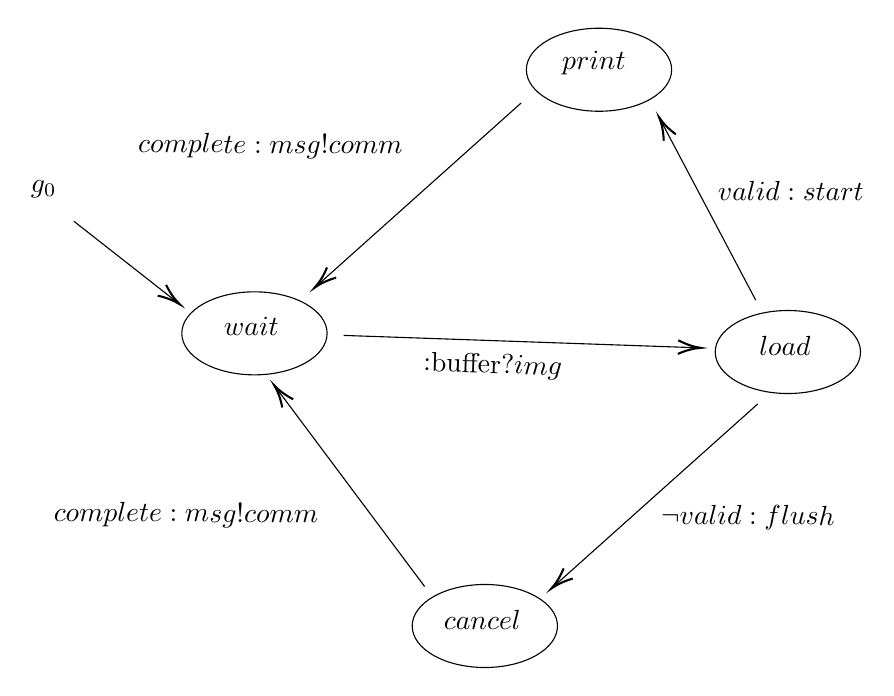
\begin{tikzpicture}[x=0.75pt,y=0.75pt,yscale=-1,xscale=1]
%uncomment if require: \path (0,331); %set diagram left start at 0, and has height of 331

%Shape: Ellipse [id:dp8321971521800935] 
\draw   (198,301) .. controls (198,289.95) and (213.67,281) .. (233,281) .. controls (252.33,281) and (268,289.95) .. (268,301) .. controls (268,312.05) and (252.33,321) .. (233,321) .. controls (213.67,321) and (198,312.05) .. (198,301) -- cycle ;
%Shape: Ellipse [id:dp9498214710995798] 
\draw   (87,160) .. controls (87,148.95) and (102.67,140) .. (122,140) .. controls (141.33,140) and (157,148.95) .. (157,160) .. controls (157,171.05) and (141.33,180) .. (122,180) .. controls (102.67,180) and (87,171.05) .. (87,160) -- cycle ;
%Shape: Ellipse [id:dp5125970438473768] 
\draw   (344,169) .. controls (344,157.95) and (359.67,149) .. (379,149) .. controls (398.33,149) and (414,157.95) .. (414,169) .. controls (414,180.05) and (398.33,189) .. (379,189) .. controls (359.67,189) and (344,180.05) .. (344,169) -- cycle ;
%Shape: Ellipse [id:dp8080305675784576] 
\draw   (253,33) .. controls (253,21.95) and (268.67,13) .. (288,13) .. controls (307.33,13) and (323,21.95) .. (323,33) .. controls (323,44.05) and (307.33,53) .. (288,53) .. controls (268.67,53) and (253,44.05) .. (253,33) -- cycle ;
%Straight Lines [id:da6100445878394302] 
\draw    (35,106) -- (84.43,144.77) ;
\draw [shift={(86,146)}, rotate = 218.11] [color={rgb, 255:red, 0; green, 0; blue, 0 }  ][line width=0.75]    (10.93,-3.29) .. controls (6.95,-1.4) and (3.31,-0.3) .. (0,0) .. controls (3.31,0.3) and (6.95,1.4) .. (10.93,3.29)   ;
%Straight Lines [id:da35540329737679166] 
\draw    (132.7,186.6) -- (204,282) ;
\draw [shift={(131.5,185)}, rotate = 53.22] [color={rgb, 255:red, 0; green, 0; blue, 0 }  ][line width=0.75]    (10.93,-3.29) .. controls (6.95,-1.4) and (3.31,-0.3) .. (0,0) .. controls (3.31,0.3) and (6.95,1.4) .. (10.93,3.29)   ;
%Straight Lines [id:da29699699994491846] 
\draw    (165,161) -- (335,166.93) ;
\draw [shift={(337,167)}, rotate = 182] [color={rgb, 255:red, 0; green, 0; blue, 0 }  ][line width=0.75]    (10.93,-3.29) .. controls (6.95,-1.4) and (3.31,-0.3) .. (0,0) .. controls (3.31,0.3) and (6.95,1.4) .. (10.93,3.29)   ;
%Straight Lines [id:da31457893798010017] 
\draw    (317.93,57.77) -- (363.5,144) ;
\draw [shift={(317,56)}, rotate = 62.15] [color={rgb, 255:red, 0; green, 0; blue, 0 }  ][line width=0.75]    (10.93,-3.29) .. controls (6.95,-1.4) and (3.31,-0.3) .. (0,0) .. controls (3.31,0.3) and (6.95,1.4) .. (10.93,3.29)   ;
%Straight Lines [id:da8819741384484475] 
\draw    (250.5,49) -- (152.49,136.67) ;
\draw [shift={(151,138)}, rotate = 318.19] [color={rgb, 255:red, 0; green, 0; blue, 0 }  ][line width=0.75]    (10.93,-3.29) .. controls (6.95,-1.4) and (3.31,-0.3) .. (0,0) .. controls (3.31,0.3) and (6.95,1.4) .. (10.93,3.29)   ;
%Straight Lines [id:da0480873078365871] 
\draw    (364.5,194) -- (266.49,281.67) ;
\draw [shift={(265,283)}, rotate = 318.19] [color={rgb, 255:red, 0; green, 0; blue, 0 }  ][line width=0.75]    (10.93,-3.29) .. controls (6.95,-1.4) and (3.31,-0.3) .. (0,0) .. controls (3.31,0.3) and (6.95,1.4) .. (10.93,3.29)   ;

% Text Node
\draw (13,85) node [anchor=north west][inner sep=0.75pt]    {$g_{0}$};
% Text Node
\draw (106,151) node [anchor=north west][inner sep=0.75pt]    {$wait$};
% Text Node
\draw (364,160) node [anchor=north west][inner sep=0.75pt]    {$load$};
% Text Node
\draw (269,23) node [anchor=north west][inner sep=0.75pt]    {$print$};
% Text Node
\draw (212,292) node [anchor=north west][inner sep=0.75pt]    {$cancel$};
% Text Node
\draw (202.31,167.58) node [anchor=north west][inner sep=0.75pt]  [rotate=-1.82]  {$\text{:buffer} ?img$};
% Text Node
\draw (344.08,85.43) node [anchor=north west][inner sep=0.75pt]  [rotate=-0.23]  {$valid:start$};
% Text Node
\draw (316.74,241.51) node [anchor=north west][inner sep=0.75pt]  [rotate=-0.23]  {$\neg valid:flush$};
% Text Node
\draw (64.75,62.43) node [anchor=north west][inner sep=0.75pt]  [rotate=-0.23]  {$complete:msg!comm$};
% Text Node
\draw (24.08,240.1) node [anchor=north west][inner sep=0.75pt]  [rotate=-0.23]  {$complete:msg!comm$};


\end{tikzpicture}}
    \caption{Program Graph example with 4 locations modeling a print server.}
    \label{fig:pg_example}
\end{figure}

Specific actions model communication among program graphs. Action $ch!x$ writes message $x$ in channel $ch$, whereas action $ch?x$ reads the message from the channel and stores it in variable $x$. In either case, the variables and messages types must be compatible. For example, in Figure~\ref{fig:pg_example}, from locations $wait$ to $load$, data is read from a channel called \textit{buffer} and stored in variable \textit{img}. As there is no guard condition before the two points, and no alternative action from location \textit{wait}, the operation always occurs when there is data on the channel.  The write operation occurs in locations \textit{print} and \textit{cancel}, where the variable \textit{msg}'s content is written in channel \textit{comm} and is available to be read by another PG within the same CS. In such a case, these operations occur when the the guard condition  \textit{complete} is satisfied.

The channel capacity \X{for} storing messages, denoted by $cap(ch)$,  is defined by its buffer size. When $cap(ch) > 0$, communication occurs asynchronously. Otherwise, \emph{handshaking} takes place, that is,  read and write operations occur synchronously. In the previous example, we have that $\mathit{cap(buffer)=0}$  to make the PG stop and wait for information arrival at channel \textit{buffer}. 

Besides, in Figure~\ref{fig:pg_example},  by executing the transition from \textit{wait} to \textit{load}, the process reads an image from the channel called \textit{buffer} and \X{stores} it in the variable \textit{img}, going from location \textit{wait} to \textit{load}. Next, the server can print \textit{img} with the image file, if the condition \textit{valid} is satisfied, i.e., $valid=true$. In such a case, the \textit{start} action is performed, and the next location reached is \textit{print}. Otherwise, identifying some problem, it cancels the operation and goes to the \textit{cancel} location, running the \textit{flush} action.

%\begin{table}[ht!]
	\small
	\fontsize{11}{11}\selectfont
	\centering
	\caption{Channels Capacity - cap(c)}
	\label{table:channel}
	
%	\begin{tabularx}{.9\textwidth}{X{0.4\linewidth}X{0.5\linewidth}}
    \begin{tabularx}{.8\textwidth}{cX}
	\hline
		
		\textbf{Capacity}
		& \textbf{Description} \\ [1ex]
	\hline	
	
	\\$cap(c)>0$ & There is a delay  between the messages transmission and receipt (Asynchronous channel)
	\\[1ex] \\
	
	\\ $cap(c)=0$ & The message transmission and receipt corresponds to a handshaking (Synchronous channel) 
	\\[1ex] \\
	\hline
	\end{tabularx}
\end{table} 




\section{Problem Statement} 
\label{sec:example}

% please consider following Prof. Rohit's guidelines for running example

% below is just a suggestion, please adapt and continue.

% we must not present the solution below! Just illustrate the problem

% Context and Explanation of the example
To motivate the addressed research problem, a simplified example of a mission execution by entities is presented. Figure~\ref{fig:example} illustrates a reconnaissance mission where a team of four UAVs is interacting in a network configuration with a central coordinator (shown in Figure~\ref{fig:example}(a)), which is responsible only for providing instructions to its subordinates. These interactions and network topology establish the Coordinated C2 approach~\citep{FRANCE2014}. The coordinator, depicted with a dashed square around it, guides the other team members to complete mission tasks. These tasks require different types of sensors for obtaining aerial images of particular points of interest, represented by red crosses.

% Highlighting the problem
The mission has some inherent risks that may lead to a change in the conditions of execution. In this example, one member of the team, marked with a dashed circle (Figure~\ref{fig:example}(b)), dropped due to some environmental change, such as an intense storm, causing damages to its motors. The loss of one entity, depicted in Figure~\ref{fig:example}(b), can potentially decrease the effectiveness and quality of the mission execution. So, a new plan is required, considering task \textit{id 0} originally assigned to the dropped drone. Otherwise, there would be a lack of C2 agility. The absence of a system strategy to maintain or increase C2 agility may compromise the amount of completed tasks at the end of execution. 


\begin{figure}[!htbp]
	\centering
	\begin{subfigure}[t]{.45\textwidth}
	\centering
	    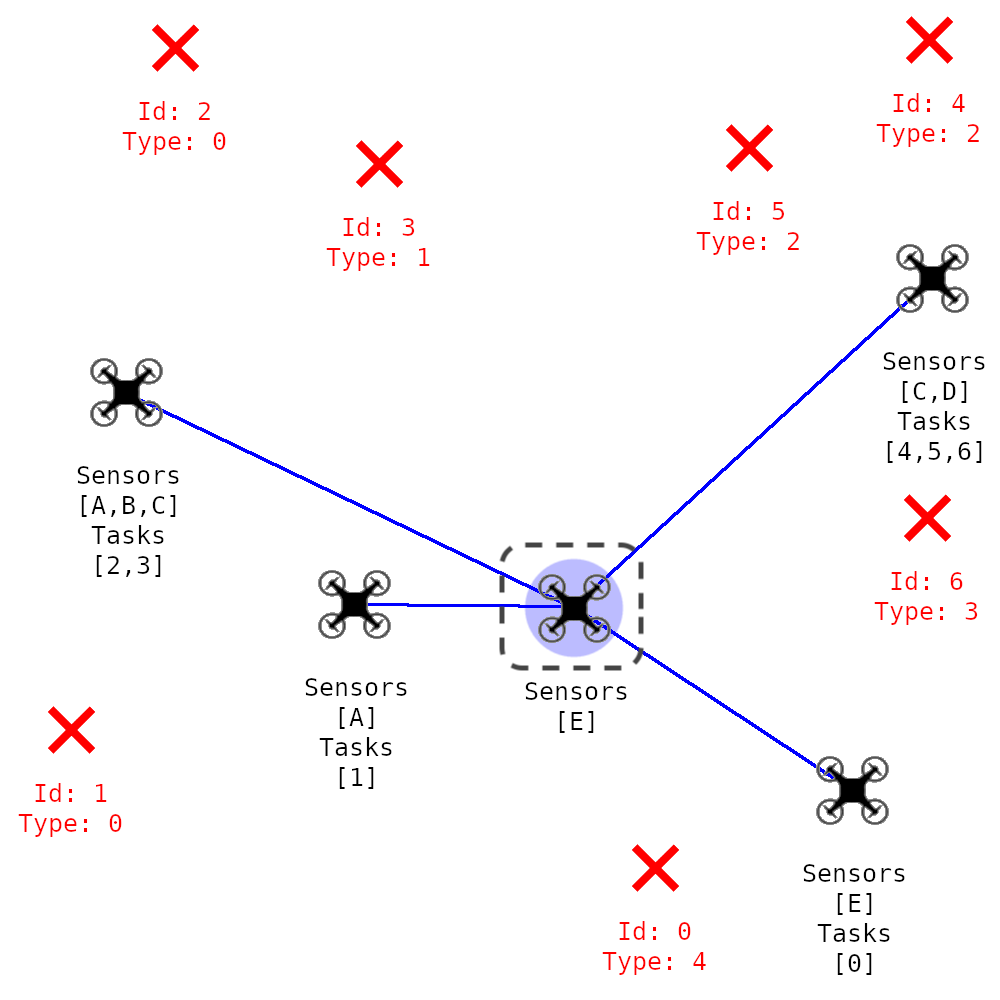
\includegraphics[width=0.95\linewidth]{img/C2Drones1-V4-dashed.png}
	    \caption{Coordinator (dashed square)\label{fig:example-a}}
	\end{subfigure}
	\begin{subfigure}[t]{.45\textwidth}
	\centering
	    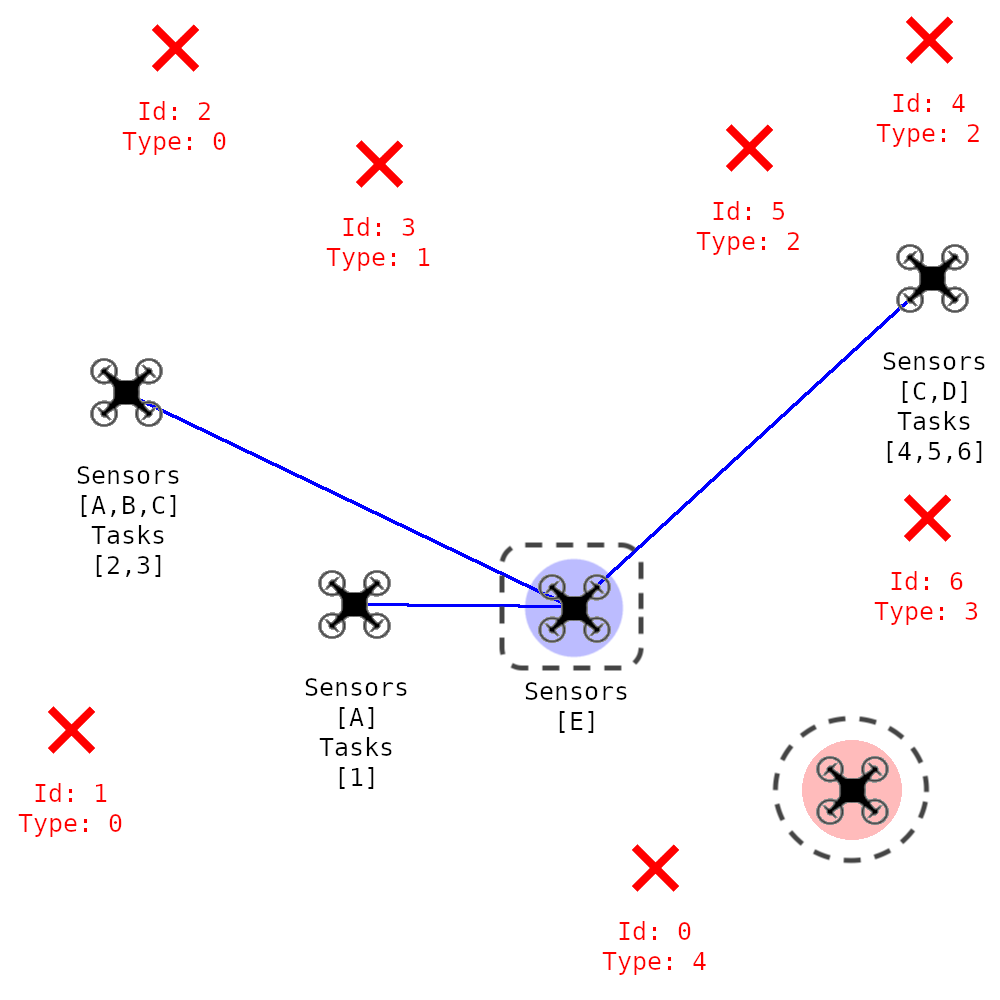
\includegraphics[width=0.95\linewidth]{img/C2Drones2-V4-dashed.png}
	    \caption{UAV dropped (dashed circle)\label{fig:example-b}}
	\end{subfigure}
	\caption{Team of entities related to a central coordinator (dashed rectangle) performing tasks at predefined locations (red crosses). A context change results in an UAV dropped (on the right, marked with a dashed circle).}
	\label{fig:example}
\end{figure}

% \begin{figure}
% \centering
% \fbox{
% \begin{minipage}{.45\textwidth}
% %\captionsetup{type=figure}
%   \centering
%   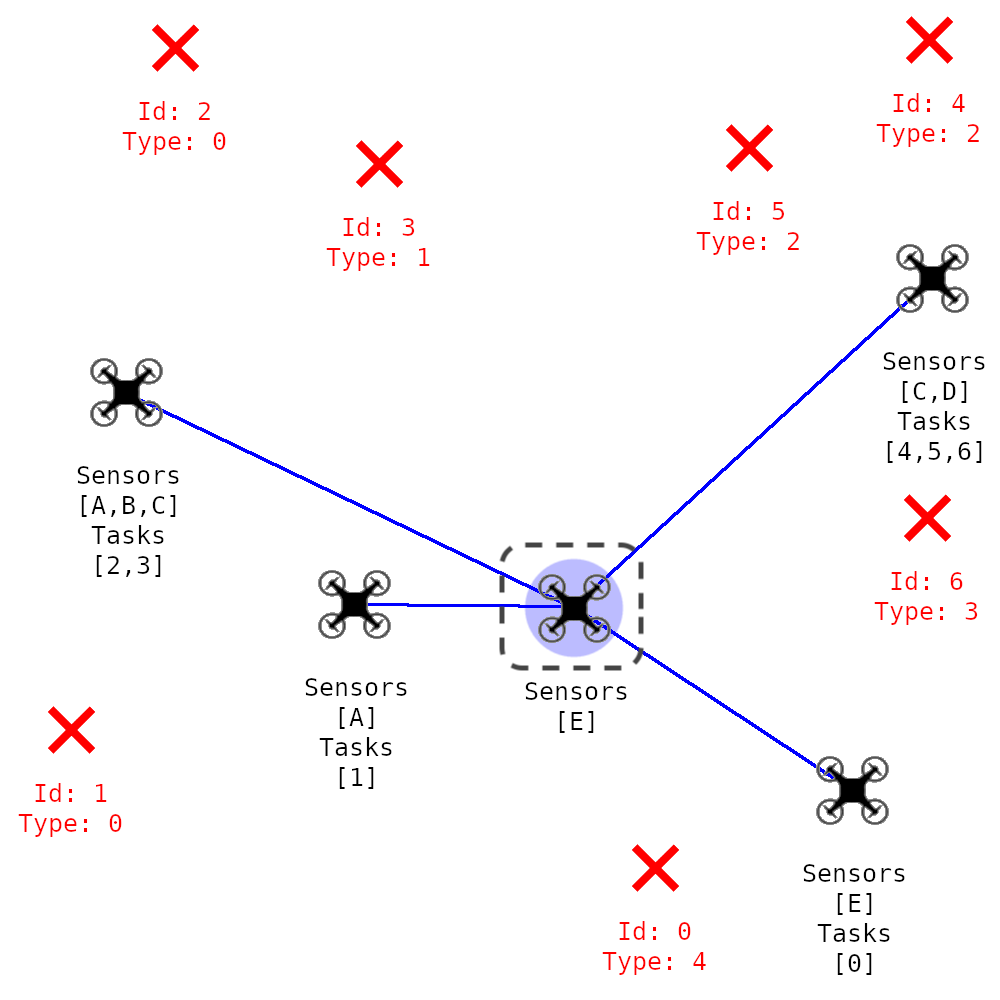
\includegraphics[width=0.95\linewidth]{img/C2Drones1-V4-dashed.png}
%   \subcaptionbox{(a) Coordinator (dashed square)\label{fig:example-a}}{}
% \end{minipage}}%
% \fbox{
% \begin{minipage}{.45\textwidth}
%   \centering
%   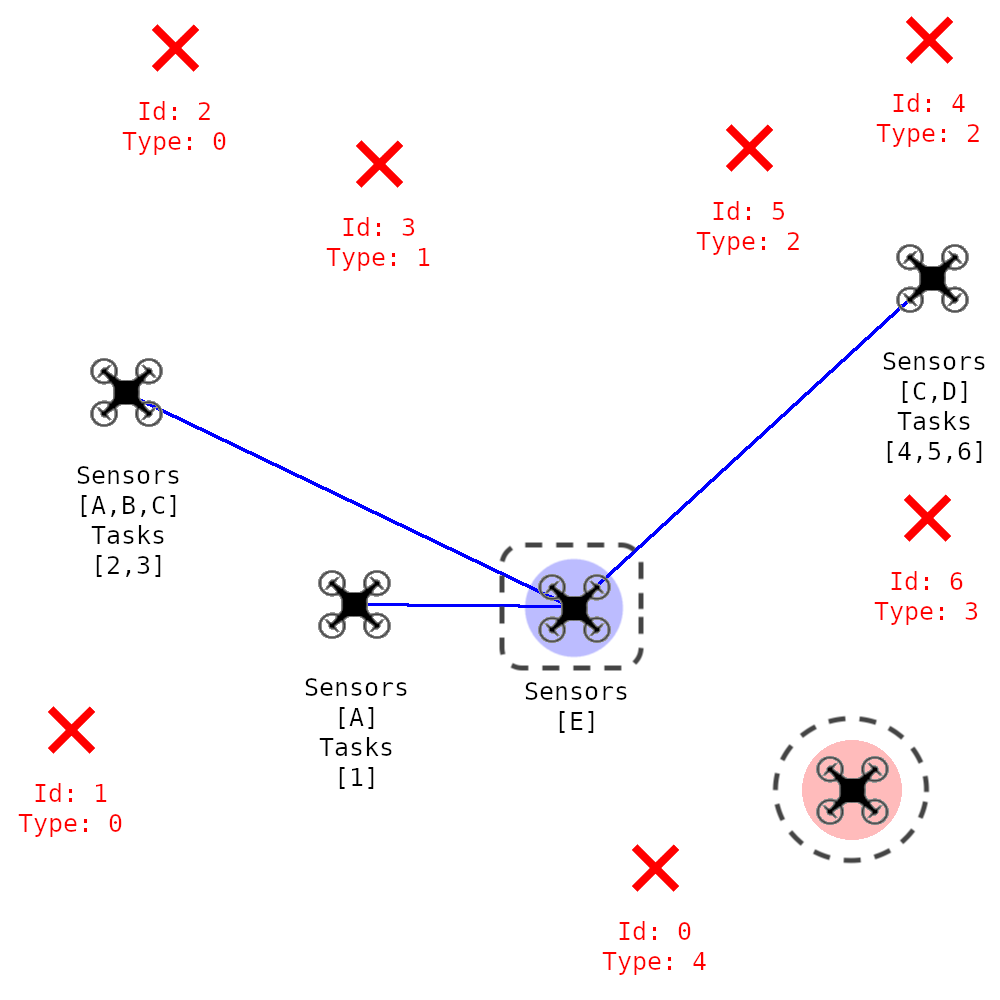
\includegraphics[width=0.95\linewidth]{img/C2Drones2-V4-dashed.png}
%   \subcaptionbox{(b) UAV dropped (dashed circle)\label{fig:example-b}}
% \end{minipage}}
% \caption{Team of entities related to a central coordinator (dashed rectangle) performing tasks at predefined locations (red crosses). A context change results in an UAV dropped (on the right, marked with a dashed circle).}
% \label{fig:example}
% \end{figure}

% Generalize the problem / Why is this not solved yet?
In general, context changes occur in the entities themselves (self) and in the environment, e.g., UAV failure, sensor damage, or weather change, and they must be considered during the mission planning.
%The self represents the entities that perform some action.
Real scenarios, where there are entities applying the available resources to accomplish a mission or to reach a goal, naturally have embedded dynamism \citep{Alberts2000, Alberts2006}. Any adaptation to the new context may decrease quality results due to an incompatibility between entities and mission, or insufficient resources to complete the mission, or even the inability to meet minimum quality acceptance level. Therefore, the C2 Agility concept introduced in Section~\ref{sec:background}, composed of C2 Approach Agility and C2 Maneuver Agility, would be compromised. This work considers a refined definition for C2 Agility as the following capability of a team in a mission:

\begin{center}
\fbox{\begin{minipage}{30em}
C2 Agility: For all tasks $t$ of a mission, it is possible to find a C2 approach $\omega$, such that a team $E$, i.e., set of members, becomes constrained to operate under $\omega$, in a way that $t$ is allocated to a member $e \in E$, and $e$ adopts  an internal configuration $c$ among its valid configurations, such that this configuration makes $e$ capable of dealing with $t$.
\end{minipage}}    
\end{center}


In other words, if there is limited C2 agility, the mission might be compromised in a dynamic context. Nevertheless, as discussed in Section~\ref{sec:relatedWork}, the state-of-art and the state-of-the-practice do not explore methodologies or strategies to provide C2 agility, especially considering context changes~\citep{Alberts2006}. 
Specifically, we consider this problem in the scope of simulation environment. This approach, which is often used to study C2 in general and in its application areas~\citep{FRANCE2014}, is relevant to explore many other scenarios such as Network Centric Warfare and telemedicine~\citep{telemedicine01, FRANCE2014, Power01}.

Even if we  represent entities’ behavior in dynamic context, modelling time constraints is outside of the scope of \X{this paper} and considered as \X{future} work. More expressive models may address such an approach, e.g., timed automata and temporal logics such as QPTL~\citep{QPTL01}. However, \X{recent works} related to C2 do not explore such a temporal aspect because of the natural complexity involved and the limitations of this field. Such works that analyze entities’ behavior in simulated and realistic \X{scenarios~\citep{FRANCE2014}}, not considering time constraints, have proven to be relevant in several domains, e.g., military.


%One possibility to avoid the problem of C2 approach agility is to change the current C2 approach, i.e., change the network configuration and leaders. Furthermore, if the team changes to an unsuitable C2 approach or is not even capable of changing its C2 approach, both cases represent a lack of C2 maneuver agility. These two types of agility compose the C2 agility concept, i.e., the entity's capability of dealing with context changes~\citep{FRANCE2014}.


%Although mission change is in the group of context changes according to \citep{Alberts10}, we are considering unchangeable set of tasks, i.e., mission does not change. We have chosen to exclude such changing of this study based on the high dependence to the strategy of how these new tasks are inserted in the system. If such tasks have a priority classification, the strategy to insert new tasks in the mission during execution can be unfeasible due to the reorganization process with a complete tasks reallocation. Such scenario in military domain is avoided due to the team resources availability~\citep{CC04}.




\section{A Product-Line Approach to C2 Agility} 
\label{sec:proposal}
To provide C2 Agility, the proposal is to present a computational model capable of representing the scenario members’ behaviors based on the roles that such elements have. To cope with context changes, these members may reconfigure themselves or adjust their coordination according to the communication structure and information exchange of a C2 strategy. This capacity is enabled by a model that allows coordination and data exchange via so called channels, and a member’s description composed by features that can be dynamically enabled according to the circumstances, generating different configurations. Particularly, the proposed computational model is a typed-parameterized extension of the channel system presented in Section~\ref{ssec:background_cs}, henceforth referred to as C2 channel system (C2CS), which is described \X{in the next} sections.



\subsection{Typed-Parameterized Channel System}
\label{sec:channelSystem}

Essentially, C2CS defines coordination among entities and their reconfiguration to cope with context changes eventually arising during a mission. These behaviors are described by three different program graphs (PGs) making up C2CS and representing role types played by entities: \textit{Task Performer (TP)}, \textit{Task Allocator (TA)}, and \textit{C2 Approach Manager (C2AM)}. TP establishes the tasks' execution and entity's reconfiguration behavior. TA defines task allocation responsibilities among entities, and C2AM specifies a C2 Approach change protocol. Types are used to describe the structure of the PG's locations as well as of the message content exchanged in synchronous and asynchronous channels. 

Figure \ref{fig:cs} depicts C2CS, whereas Equation~\ref{eq:cs} defines it. The use of channel system concepts allows the execution of parallel processes with communication capability among them. Such a structure allows us to model the identified roles in a C2 system running in parallel and performing information exchange. This exchange leverages channels, i.e., first-in, first-out buffers that carry messages. The C2CS employs both synchronous and asynchronous channels. The former, e.g., $ch_2$ and $ch_3$, synchronizes C2AM's and TA's PG when they perform tasks allocation and C2 Approach change. The latter, e.g., $m_k$ and $ch_1$, enables the transmission of allocated tasks to the TPs and the return of not possible tasks to the TA. 

\begin{figure}[ht]
    \centering
    \scalebox{.8}{

\tikzset{every picture/.style={line width=0.75pt}} %set default line width to 0.75pt        

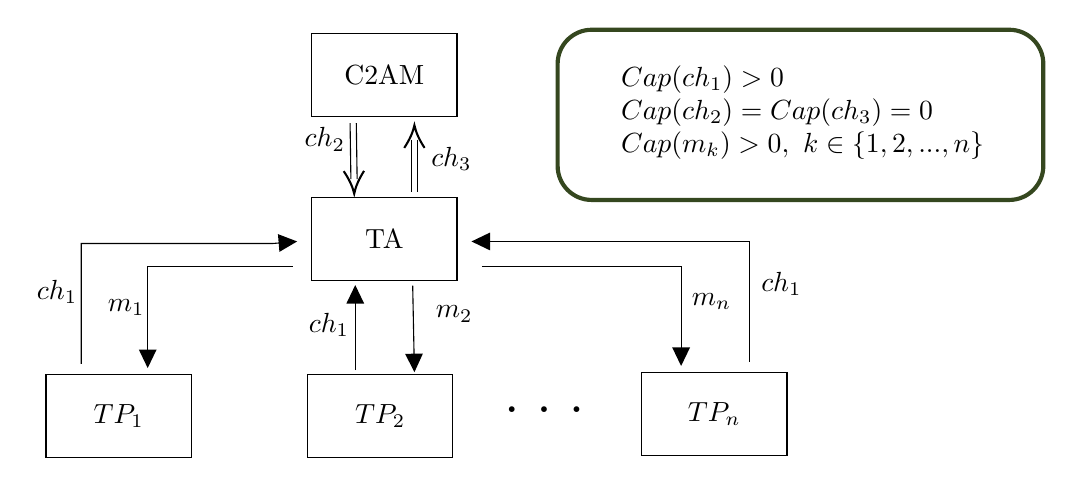
\begin{tikzpicture}[x=0.75pt,y=0.75pt,yscale=-1,xscale=1]
%uncomment if require: \path (0,225); %set diagram left start at 0, and has height of 225

%Shape: Rectangle [id:dp7793135649662085] 
\draw   (146,89) -- (216,89) -- (216,129) -- (146,129) -- cycle ;
%Shape: Rectangle [id:dp8388066725390221] 
\draw   (146,10) -- (216,10) -- (216,50) -- (146,50) -- cycle ;
%Shape: Rectangle [id:dp48691256180587716] 
\draw   (18,174) -- (88,174) -- (88,214) -- (18,214) -- cycle ;
%Straight Lines [id:da7136052167478543] 
\draw    (194.67,131.33) -- (195.44,170) ;
\draw [shift={(195.5,173)}, rotate = 268.85] [fill={rgb, 255:red, 0; green, 0; blue, 0 }  ][line width=0.08]  [draw opacity=0] (8.93,-4.29) -- (0,0) -- (8.93,4.29) -- cycle    ;
%Straight Lines [id:da1199439366931846] 
\draw    (35,169) -- (35,111) -- (127,111) -- (136.01,110.25) ;
\draw [shift={(139,110)}, rotate = 535.24] [fill={rgb, 255:red, 0; green, 0; blue, 0 }  ][line width=0.08]  [draw opacity=0] (8.93,-4.29) -- (0,0) -- (8.93,4.29) -- cycle    ;
%Shape: Rectangle [id:dp8070909053866772] 
\draw   (305,173) -- (375,173) -- (375,213) -- (305,213) -- cycle ;
%Shape: Rectangle [id:dp18131918632628874] 
\draw   (144,174) -- (214,174) -- (214,214) -- (144,214) -- cycle ;
%Straight Lines [id:da23459308482895536] 
\draw    (357,168) -- (357,110) -- (226,110) ;
\draw [shift={(223,110)}, rotate = 360] [fill={rgb, 255:red, 0; green, 0; blue, 0 }  ][line width=0.08]  [draw opacity=0] (8.93,-4.29) -- (0,0) -- (8.93,4.29) -- cycle    ;
%Straight Lines [id:da9340034396500284] 
\draw    (228,122) -- (324,122) -- (324,167) ;
\draw [shift={(324,170)}, rotate = 270] [fill={rgb, 255:red, 0; green, 0; blue, 0 }  ][line width=0.08]  [draw opacity=0] (8.93,-4.29) -- (0,0) -- (8.93,4.29) -- cycle    ;
%Straight Lines [id:da26523318096149495] 
\draw    (137,122) -- (67,122) -- (67,168) ;
\draw [shift={(67,171)}, rotate = 270] [fill={rgb, 255:red, 0; green, 0; blue, 0 }  ][line width=0.08]  [draw opacity=0] (8.93,-4.29) -- (0,0) -- (8.93,4.29) -- cycle    ;
%Straight Lines [id:da6224238934860249] 
\draw    (167,172) -- (167,134) ;
\draw [shift={(167,131)}, rotate = 450] [fill={rgb, 255:red, 0; green, 0; blue, 0 }  ][line width=0.08]  [draw opacity=0] (8.93,-4.29) -- (0,0) -- (8.93,4.29) -- cycle    ;
%Straight Lines [id:da30878293142018354] 
\draw    (167.5,52.98) -- (167.9,79.98)(164.5,53.02) -- (164.9,80.02) ;
\draw [shift={(166.5,87)}, rotate = 269.15999999999997] [color={rgb, 255:red, 0; green, 0; blue, 0 }  ][line width=0.75]    (10.93,-4.9) .. controls (6.95,-2.3) and (3.31,-0.67) .. (0,0) .. controls (3.31,0.67) and (6.95,2.3) .. (10.93,4.9)   ;
%Straight Lines [id:da1036410124215259] 
\draw    (197,61) -- (197,86)(194,61) -- (194,86) ;
\draw [shift={(195.5,54)}, rotate = 90] [color={rgb, 255:red, 0; green, 0; blue, 0 }  ][line width=0.75]    (10.93,-4.9) .. controls (6.95,-2.3) and (3.31,-0.67) .. (0,0) .. controls (3.31,0.67) and (6.95,2.3) .. (10.93,4.9)   ;
%Rounded Rect [id:dp17275257935630328] 
\draw  [color={rgb, 255:red, 53; green, 71; blue, 31 }  ,draw opacity=1 ][line width=1.5]  (264.5,24.4) .. controls (264.5,15.34) and (271.84,8) .. (280.9,8) -- (482.1,8) .. controls (491.16,8) and (498.5,15.34) .. (498.5,24.4) -- (498.5,73.6) .. controls (498.5,82.66) and (491.16,90) .. (482.1,90) -- (280.9,90) .. controls (271.84,90) and (264.5,82.66) .. (264.5,73.6) -- cycle ;

% Text Node
\draw (181,30) node   [align=left] {C2AM};
% Text Node
\draw (181,109) node   [align=left] {TA};
% Text Node
\draw (53,194) node    {$TP_{1}$};
% Text Node
\draw (23.33,134.33) node    {$ch_{1}$};
% Text Node
\draw (214.67,145) node    {$m_{2}$};
% Text Node
\draw (340,193) node    {$TP_{n}$};
% Text Node
\draw (179,194) node    {$TP_{2}$};
% Text Node
\draw (258,191) node  [font=\Large] [align=left] {\textbf{. . .}};
% Text Node
\draw (338.67,139) node    {$m_{n}$};
% Text Node
\draw (56.67,142) node    {$m_{1}$};
% Text Node
\draw (154.33,150.33) node    {$ch_{1}$};
% Text Node
\draw (372.33,130.33) node    {$ch_{1}$};
% Text Node
\draw (152.33,60.83) node    {$ch_{2}$};
% Text Node
\draw (213.33,70.33) node    {$ch_{3}$};
% Text Node
\draw (382.5,48) node    {$ \begin{array}{l}
Cap( ch_{1})  >0\\
Cap( ch_{2}) =Cap( ch_{3}) =0\\
Cap( m_{k})  >0,\ k\in \{1,2,...,n\}
\end{array}$};


\end{tikzpicture}}
    \caption{C2 Channel System for a team composed by \textit{n} members with the TP role asynchronous and synchronous channels represented by single and double line arrows, respectively.}
    \label{fig:cs}
\end{figure}


\begin{equation}
    \label{eq:cs}
    \begin{split}
    C2CS([FM]\ E,\ &  \mathcal{P}(Task)\ M,\ C2_{ap}\ \omega_0) = [C2AM(E, M,\omega_0)\ |\ TA\ | \\ & \ TP(fm_1, \omega_0)\ |\ ...\ |\ TP(fm_n, \omega_0)]
    \end{split}
\end{equation}

\color{black}
In Equation~\ref{eq:cs}, the parameters have the following meaning and types. The set $M=\{t_1, t_2,\ ...,\ t_m \}$ is the designated mission, consisting of tasks that the members will try to perform. $M$ belongs to $\mathcal{P}(Task)$, which is the power set of $Task$, where $Task=\{t_a, t_b,\ ...,\ t_z \}$ is the set of all possible tasks. The list $E = [fm_1, fm_2,\ ...,\ fm_n ]$ of team members is such that each team member has a capability of type Feature Model ($FM$). Additionally, such members always operate a C2 Approach $\omega_0 \in \Omega$, where $\Omega =$ \textit{\{Edge, Collaborative, Coordinated, De-Conflicted, Conflicted\}}. Lastly, the vertical bars represent parallel composition of the PGs representing the roles played by the team members.
\color{black}

C2CS leverages parameters to abstract from specific mission, entities, and initial conditions. It models roles that will be performed by the agents.

Each role played by the entities is represented by a PG that receives parameters that define some aspects of its internal structure. Such PGs are parallel processes that compose the C2CS and are instantiated according to the C2 Approach selected. Instances of different PGs can coexist in the same member according to the C2 Approach operated. In particular, the representation of multiple TPs shown in Figure~\ref{fig:cs} is to emphasize the existence of a specific asynchronous channel $m_k$ for each member $k$ owning a TP role instance, from where they receive the tasks to be performed. All members within $E$ with such a role instance are responsible for the mission's tasks accomplishment. Based on this, the member-to-role-instance mapping is such that each team member may eventually play one instance of the TP, TA, and C2AM roles simultaneously, and more details related to the implementation of this mapping are available in a public repository\footnote{\gitRepository}.
   
 
%The member-to-role-instance mapping is such that each team member plays each EX role instance, and it contributes \textit{partially} to both the TA and the C2A roles, the amount of such contribution depending on the current C2 approach. Conversely, each EX role instance is cohesively encapsulated in one member, whereas the C2A and the TA roles are \textit{scattered} throughout team members, given the inherent collaborative nature of these roles.  it.
%Team members contribute to all roles with dynamic intensity during the mission. 

In a typical C2CS scenario, when the mission starts, TA allocates tasks to team members, which work on accomplishing them. Eventually, to handle context changes, members may reconfigure themselves, e.g., due to sensor failure, or \color{black}the TA \color{black} can reallocate tasks among members, e.g., due to member failure. Alternatively, even a task allocation might not suffice, in which case the C2AM might change the C2 approach, prompting new task allocation among members. \color{black}In the worst scenario, when changing the C2 approach does not suffice, the task fails.\color{black} 


Recalling the motivating example (Section~\ref{sec:example}), in that specific C2 approach the coordinator plays the C2AM and TA roles. Each one of the other members plays the TP role. In that particular case, the loss of one member will first prompt the leader to reallocate tasks to the other team members, using the channels depicted in Figure \ref{fig:example2-a}. 
 Since the only member capable of executing the task that was previously allocated to the lost member is the leader, the C2AM changes the current C2 approach to Edge \citep{FRANCE2014}, prompting this modification using the communication network among members, i.e., the C2 Approach. This way, the former leader now plays the TP role and thus can execute the aforementioned tasks. This resulting situation is illustrated in Figure \ref{fig:example2-b}.

\begin{figure}[!htbp]
	\centering
	\begin{subfigure}[t]{.45\textwidth}
	\centering
	    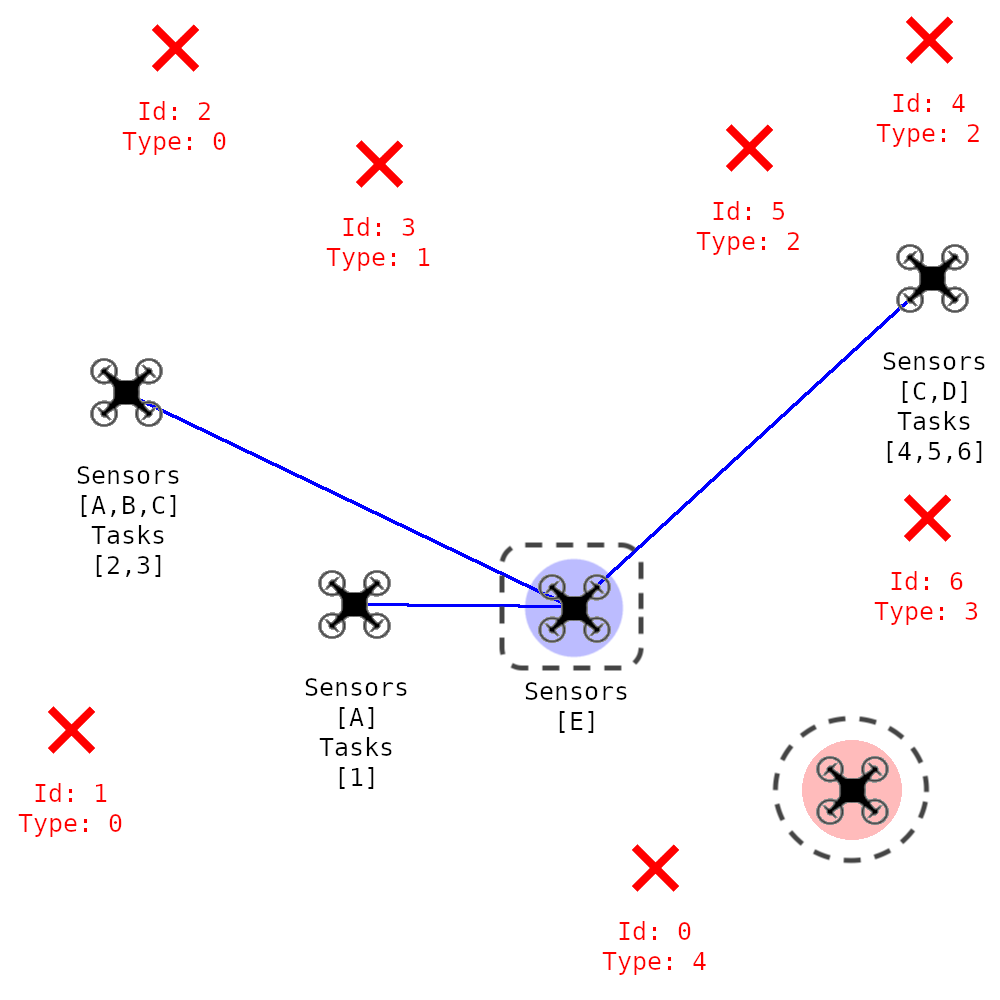
\includegraphics[width=0.95\linewidth]{img/C2Drones2-V4-dashed.png}
	    \caption{UAV dropped (dashed circle)\label{fig:example2-a}}
	\end{subfigure}
	\begin{subfigure}[t]{.45\textwidth}
	\centering
	    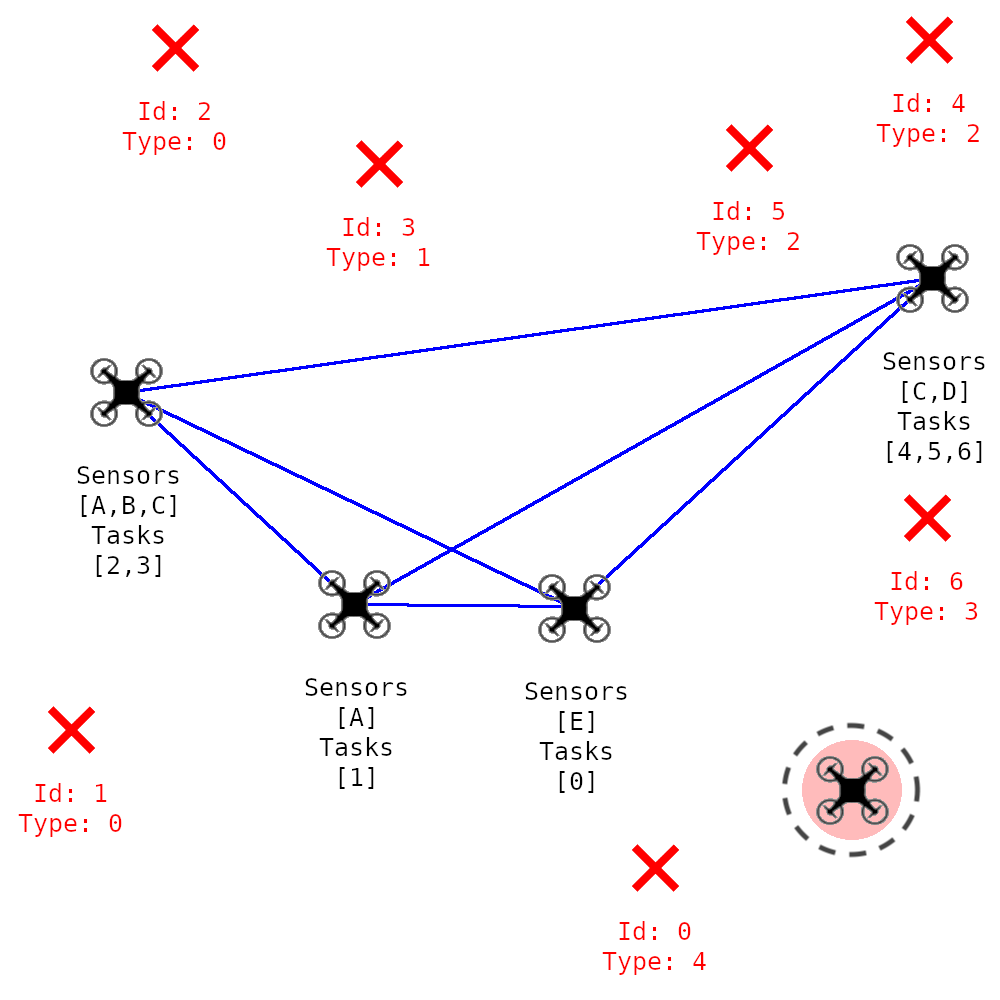
\includegraphics[width=0.95\linewidth]{img/C2Drones3-V4-dashed.png}
	    \caption{C2 Approach change \label{fig:example2-b}}
	\end{subfigure}
	\caption{The team performing tasks after C2 Approach change (lines indicating communication links) due to problems with one of the members (dropped UAV marked with a dashed circle)}
	\label{fig:TeamExecutionAfterManuever}
\end{figure}

% \begin{figure}
% \centering
% \fbox{
% \begin{minipage}{.45\textwidth}
% %\captionsetup{type=figure}
%   \centering
%   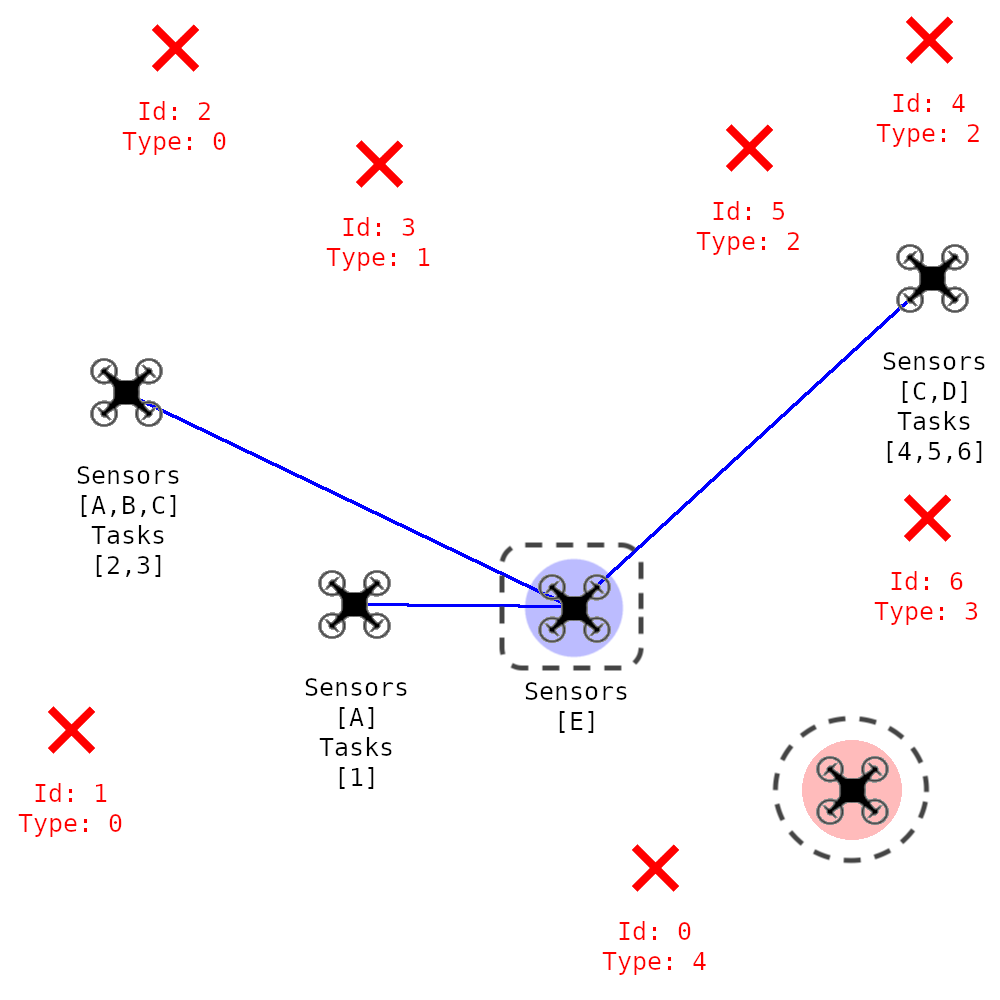
\includegraphics[width=0.95\linewidth]{img/C2Drones2-V4-dashed.png}
%   \subcaptionbox{(a) UAV dropped (dashed circle)\label{fig:example2-a}}{}
% \end{minipage}}%
% \fbox{
% \begin{minipage}{.45\textwidth}
%   \centering
%   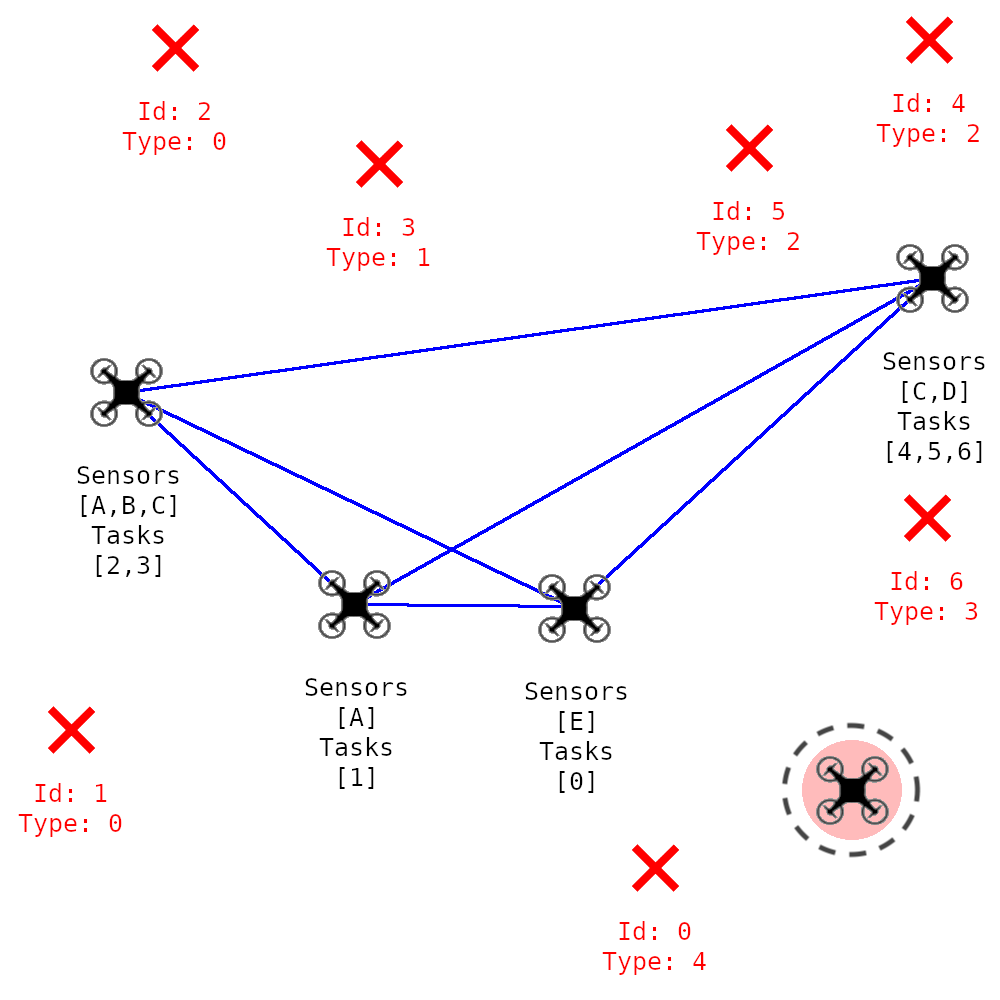
\includegraphics[width=0.95\linewidth]{img/C2Drones3-V4-dashed.png}
%   \subcaptionbox{(b) C2 Approach change \label{fig:example2-b}}{}
% \end{minipage}}
% \caption{The team performing tasks after C2 Approach change (lines indicating communication links) due to problems with one of the members (dropped UAV marked with a dashed circle)}
% \label{fig:example}
% \end{figure}


%\begin{figure}[ht]
%    \centering
%    \fbox{
%    \begin{minipage}{.45\textwidth}
%  \centering
%  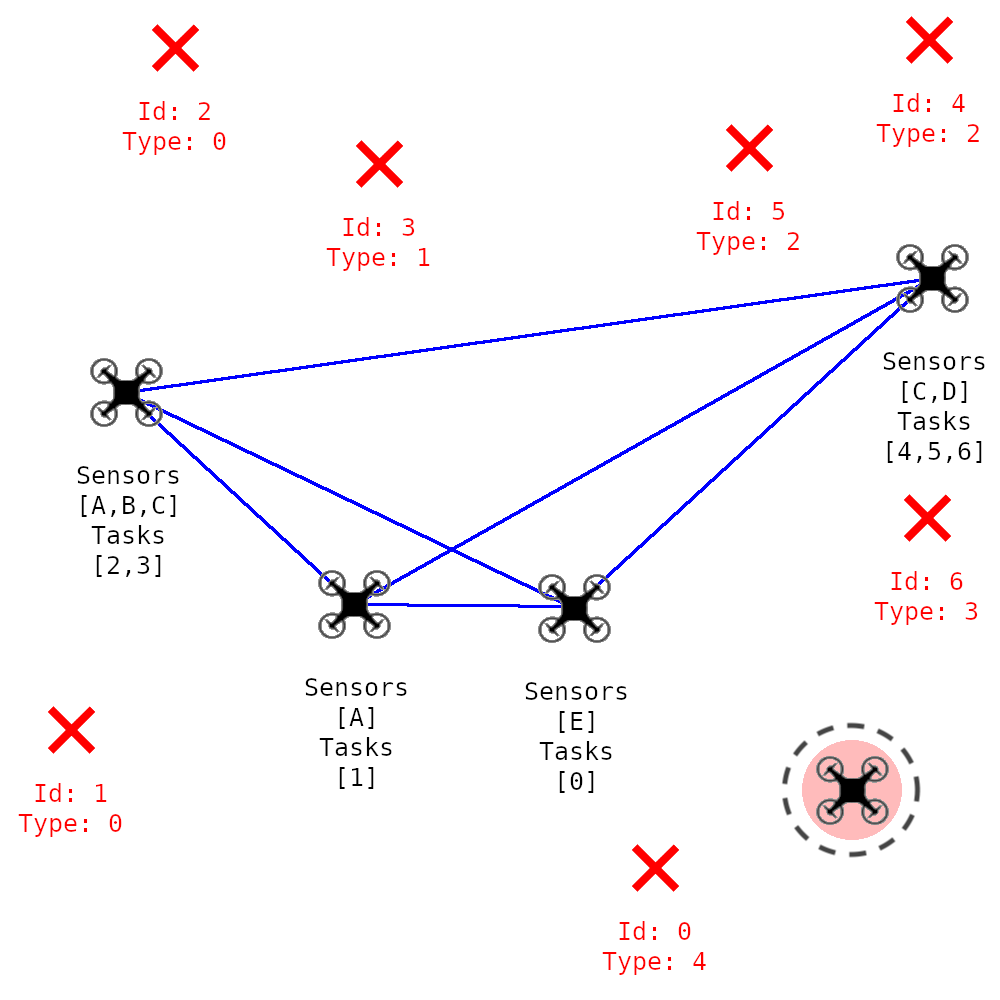
\includegraphics[width=0.95\linewidth]{img/C2Drones3-V4-dashed.png}
%\end{minipage}}
%\caption{The team performing tasks after C2 Approach change(lines indicating communication) due to problems with one of the members(marked with a dashed circle)}
%\label{fig:3TeamExecutionAfterManuever}
%\end{figure}

Overall, reconfiguration, performing new task allocation, and changing the C2 approach under certain context changes are explicitly represented in the PGs, \color{black}thereby enabling the C2CS's strategy \color{black} to achieve agility (cf. Section~\ref{sec:example}). The PGs are detailed in the following, and their implementation is publicly available elsewhere.\footnote{\implementation}

\X{In summary, Figure~\ref{fig:diagram} shows the interaction between these roles played by the members. The tasks received by the member with the role \emph{C2AM} causes an initial C2 approach selection, followed by the members notification. Next, the \emph{TA} role receives the tasks and performs the allocation. In case of no suitable allocation, the system tries to change the C2 approach to improve the awareness. All allocated tasks are sent to the related TP. This member tries to find a suitable configuration. If it is not possible, the task is reallocated. Finally, in case of context changes, the \emph{TA} and the \emph{TP} roles try to adjust themselves. A new configuration is first tried, followed by task reallocation if the configuration does not suffice. In case they do not work, a new C2 approach is evaluated to obtain a suitable system awareness.
}


\begin{figure}[!ht]
    \centering
    \scalebox{.75}{

\tikzset{every picture/.style={line width=0.75pt}} %set default line width to 0.75pt        

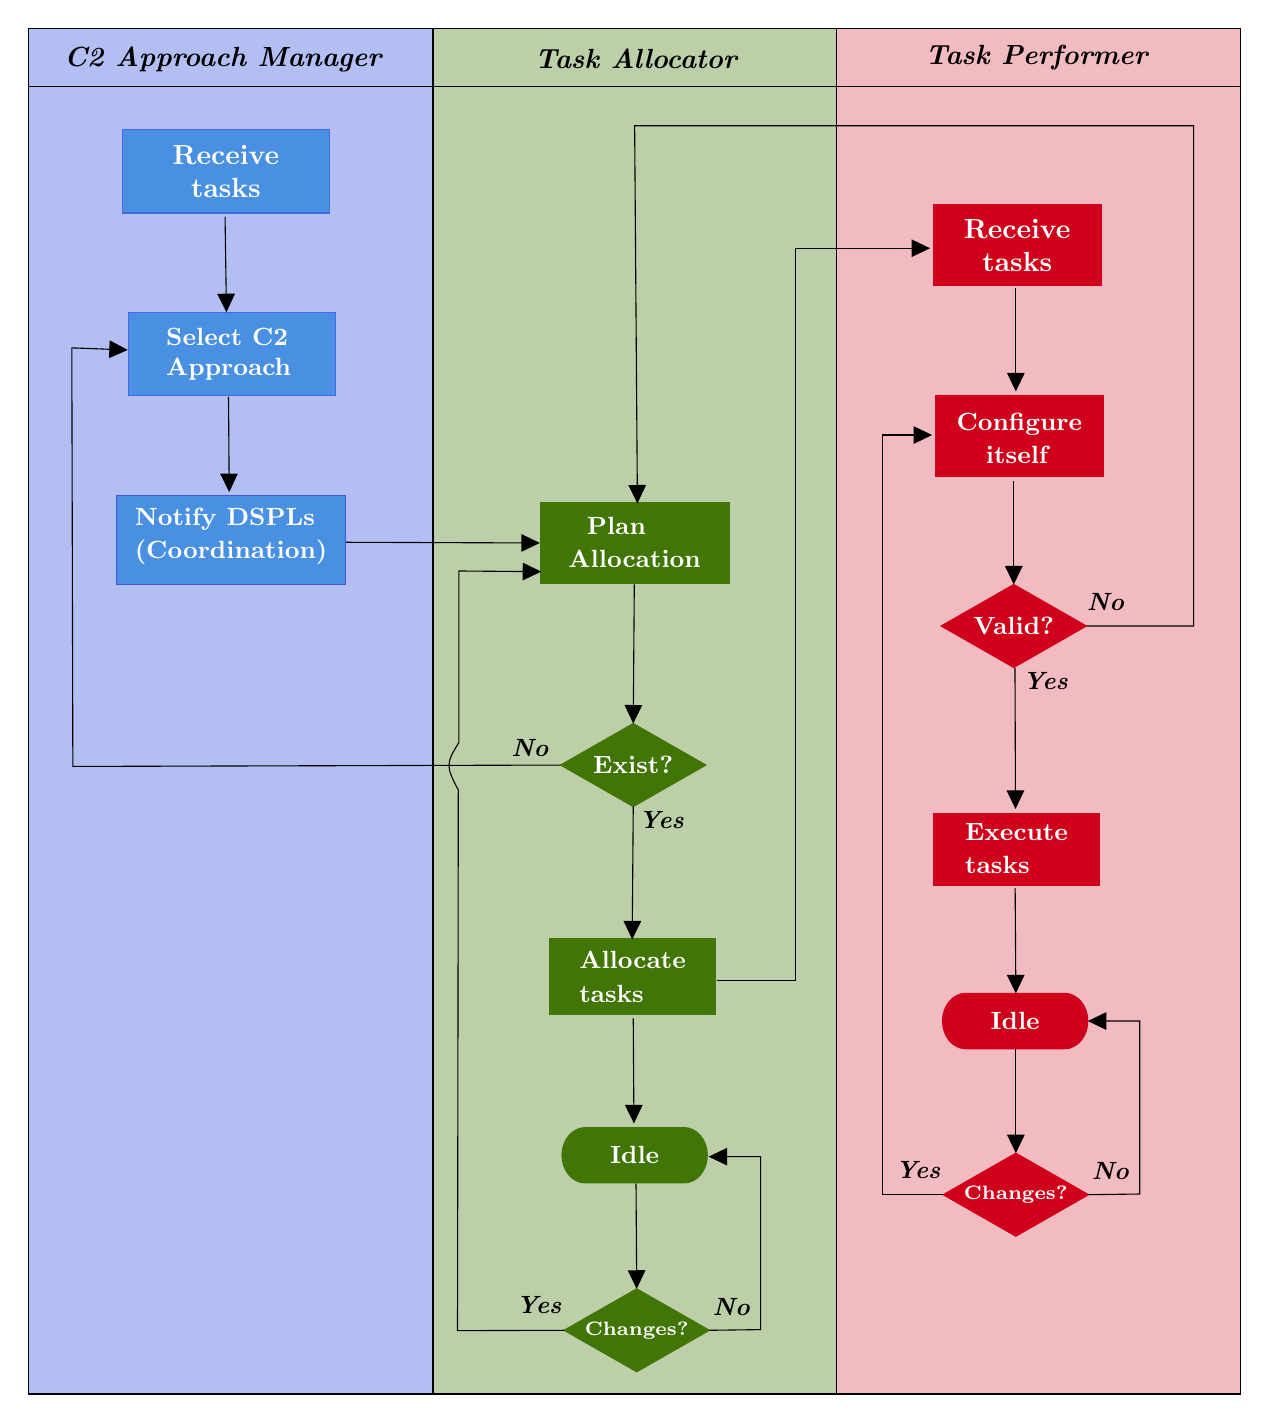
\begin{tikzpicture}[x=0.75pt,y=0.75pt,yscale=-1,xscale=1]
%uncomment if require: \path (0,673); %set diagram left start at 0, and has height of 673

%Shape: Rectangle [id:dp8854253159391561] 
\draw  [fill={rgb, 255:red, 74; green, 102; blue, 226 }  ,fill opacity=0.42 ] (2.5,3) -- (197.5,3) -- (197.5,661) -- (2.5,661) -- cycle ;
%Shape: Rectangle [id:dp3469463448197052] 
\draw  [fill={rgb, 255:red, 65; green, 117; blue, 5 }  ,fill opacity=0.35 ] (197.5,3) -- (392,3) -- (392,661) -- (197.5,661) -- cycle ;
%Shape: Rectangle [id:dp018917795120609204] 
\draw  [fill={rgb, 255:red, 208; green, 2; blue, 27 }  ,fill opacity=0.27 ] (392,3) -- (586.67,3) -- (586.67,661) -- (392,661) -- cycle ;
%Straight Lines [id:da8146359528310543] 
\draw    (2.5,31) -- (587,31) ;
%Flowchart: Process [id:dp15412574148578628] 
\draw  [color={rgb, 255:red, 74; green, 104; blue, 226 }  ,draw opacity=1 ][fill={rgb, 255:red, 74; green, 144; blue, 226 }  ,fill opacity=1 ] (51,140) -- (150.5,140) -- (150.5,180) -- (51,180) -- cycle ;
%Flowchart: Process [id:dp48065105856176205] 
\draw  [color={rgb, 255:red, 74; green, 83; blue, 226 }  ,draw opacity=1 ][fill={rgb, 255:red, 74; green, 144; blue, 226 }  ,fill opacity=1 ] (45,228.17) -- (155.5,228.17) -- (155.5,270.83) -- (45,270.83) -- cycle ;
%Flowchart: Process [id:dp6629894570275567] 
\draw  [color={rgb, 255:red, 65; green, 117; blue, 5 }  ,draw opacity=1 ][fill={rgb, 255:red, 65; green, 117; blue, 5 }  ,fill opacity=1 ] (249.17,231.33) -- (340.17,231.33) -- (340.17,270.33) -- (249.17,270.33) -- cycle ;
%Flowchart: Decision [id:dp5160918625824323] 
\draw  [color={rgb, 255:red, 65; green, 117; blue, 5 }  ,draw opacity=1 ][fill={rgb, 255:red, 65; green, 117; blue, 5 }  ,fill opacity=1 ] (294,338) -- (329,358) -- (294,378) -- (259,358) -- cycle ;
%Flowchart: Process [id:dp8044553855974566] 
\draw  [color={rgb, 255:red, 65; green, 117; blue, 5 }  ,draw opacity=1 ][fill={rgb, 255:red, 65; green, 117; blue, 5 }  ,fill opacity=1 ] (253.67,441.67) -- (333.67,441.67) -- (333.67,478.33) -- (253.67,478.33) -- cycle ;
%Straight Lines [id:da6701074801455137] 
\draw    (259,358) -- (24,358.67) -- (23.5,157) -- (47.5,157.89) ;
\draw [shift={(50.5,158)}, rotate = 182.12] [fill={rgb, 255:red, 0; green, 0; blue, 0 }  ][line width=0.08]  [draw opacity=0] (8.93,-4.29) -- (0,0) -- (8.93,4.29) -- cycle    ;
%Straight Lines [id:da6383024146874764] 
\draw    (294,378) -- (293.52,439) ;
\draw [shift={(293.5,442)}, rotate = 270.45] [fill={rgb, 255:red, 0; green, 0; blue, 0 }  ][line width=0.08]  [draw opacity=0] (8.93,-4.29) -- (0,0) -- (8.93,4.29) -- cycle    ;
%Straight Lines [id:da7026427833669057] 
\draw    (294.5,271) -- (294.02,335) ;
\draw [shift={(294,338)}, rotate = 270.43] [fill={rgb, 255:red, 0; green, 0; blue, 0 }  ][line width=0.08]  [draw opacity=0] (8.93,-4.29) -- (0,0) -- (8.93,4.29) -- cycle    ;
%Straight Lines [id:da7965236156041576] 
\draw    (155.67,250.67) -- (246,250.99) ;
\draw [shift={(249,251)}, rotate = 180.2] [fill={rgb, 255:red, 0; green, 0; blue, 0 }  ][line width=0.08]  [draw opacity=0] (8.93,-4.29) -- (0,0) -- (8.93,4.29) -- cycle    ;
%Straight Lines [id:da4788721755855869] 
\draw    (97.33,93.83) -- (97.96,136.83) ;
\draw [shift={(98,139.83)}, rotate = 269.17] [fill={rgb, 255:red, 0; green, 0; blue, 0 }  ][line width=0.08]  [draw opacity=0] (8.93,-4.29) -- (0,0) -- (8.93,4.29) -- cycle    ;
%Straight Lines [id:da7999024493741219] 
\draw    (99,180.67) -- (99.31,223.5) ;
\draw [shift={(99.33,226.5)}, rotate = 269.58] [fill={rgb, 255:red, 0; green, 0; blue, 0 }  ][line width=0.08]  [draw opacity=0] (8.93,-4.29) -- (0,0) -- (8.93,4.29) -- cycle    ;
%Shape: Rectangle [id:dp4479174596462915] 
\draw  [color={rgb, 255:red, 208; green, 2; blue, 27 }  ,draw opacity=1 ][fill={rgb, 255:red, 208; green, 2; blue, 27 }  ,fill opacity=1 ] (439.5,180) -- (520.5,180) -- (520.5,219) -- (439.5,219) -- cycle ;
%Flowchart: Process [id:dp18610523674883006] 
\draw  [color={rgb, 255:red, 208; green, 2; blue, 27 }  ,draw opacity=1 ][fill={rgb, 255:red, 208; green, 2; blue, 27 }  ,fill opacity=1 ] (438.67,381.33) -- (518.67,381.33) -- (518.67,416) -- (438.67,416) -- cycle ;
%Flowchart: Terminator [id:dp6793353293966301] 
\draw  [color={rgb, 255:red, 208; green, 2; blue, 27 }  ,draw opacity=1 ][fill={rgb, 255:red, 208; green, 2; blue, 27 }  ,fill opacity=1 ] (454.2,468) -- (501.8,468) .. controls (507.99,468) and (513,473.97) .. (513,481.33) .. controls (513,488.7) and (507.99,494.67) .. (501.8,494.67) -- (454.2,494.67) .. controls (448.01,494.67) and (443,488.7) .. (443,481.33) .. controls (443,473.97) and (448.01,468) .. (454.2,468) -- cycle ;
%Straight Lines [id:da16428269292090503] 
\draw    (512.33,291) -- (564,291) -- (564,50) -- (294.67,50) -- (295.98,229) ;
\draw [shift={(296,232)}, rotate = 269.58] [fill={rgb, 255:red, 0; green, 0; blue, 0 }  ][line width=0.08]  [draw opacity=0] (8.93,-4.29) -- (0,0) -- (8.93,4.29) -- cycle    ;
%Straight Lines [id:da6031633731040735] 
\draw    (477.92,311.17) -- (478.16,376.17) ;
\draw [shift={(478.17,379.17)}, rotate = 269.79] [fill={rgb, 255:red, 0; green, 0; blue, 0 }  ][line width=0.08]  [draw opacity=0] (8.93,-4.29) -- (0,0) -- (8.93,4.29) -- cycle    ;
%Straight Lines [id:da15605132192013493] 
\draw    (477.33,221) -- (477.33,268) ;
\draw [shift={(477.33,271)}, rotate = 270] [fill={rgb, 255:red, 0; green, 0; blue, 0 }  ][line width=0.08]  [draw opacity=0] (8.93,-4.29) -- (0,0) -- (8.93,4.29) -- cycle    ;
%Straight Lines [id:da8423233165938356] 
\draw    (478,417.33) -- (478.31,465) ;
\draw [shift={(478.33,468)}, rotate = 269.62] [fill={rgb, 255:red, 0; green, 0; blue, 0 }  ][line width=0.08]  [draw opacity=0] (8.93,-4.29) -- (0,0) -- (8.93,4.29) -- cycle    ;
%Flowchart: Decision [id:dp6377795539825191] 
\draw  [color={rgb, 255:red, 208; green, 2; blue, 27 }  ,draw opacity=1 ][fill={rgb, 255:red, 208; green, 2; blue, 27 }  ,fill opacity=1 ] (477.33,271) -- (512.33,291) -- (477.33,311) -- (442.33,291) -- cycle ;
%Shape: Rectangle [id:dp5849638253268429] 
\draw  [color={rgb, 255:red, 208; green, 2; blue, 27 }  ,draw opacity=1 ][fill={rgb, 255:red, 208; green, 2; blue, 27 }  ,fill opacity=1 ] (438.5,88) -- (519.5,88) -- (519.5,127) -- (438.5,127) -- cycle ;

%Straight Lines [id:da2345904096698579] 
\draw    (478.33,128) -- (478.33,175) ;
\draw [shift={(478.33,178)}, rotate = 270] [fill={rgb, 255:red, 0; green, 0; blue, 0 }  ][line width=0.08]  [draw opacity=0] (8.93,-4.29) -- (0,0) -- (8.93,4.29) -- cycle    ;
%Straight Lines [id:da7015511994830441] 
\draw    (334.33,462) -- (372,462) -- (372,109) -- (404,109) -- (434,109) ;
\draw [shift={(437,109)}, rotate = 180] [fill={rgb, 255:red, 0; green, 0; blue, 0 }  ][line width=0.08]  [draw opacity=0] (8.93,-4.29) -- (0,0) -- (8.93,4.29) -- cycle    ;
%Straight Lines [id:da3061614783569826] 
\draw    (478.33,495) -- (478.33,542) ;
\draw [shift={(478.33,545)}, rotate = 270] [fill={rgb, 255:red, 0; green, 0; blue, 0 }  ][line width=0.08]  [draw opacity=0] (8.93,-4.29) -- (0,0) -- (8.93,4.29) -- cycle    ;
%Flowchart: Decision [id:dp9836915912197407] 
\draw  [color={rgb, 255:red, 208; green, 2; blue, 27 }  ,draw opacity=1 ][fill={rgb, 255:red, 208; green, 2; blue, 27 }  ,fill opacity=1 ] (478.33,545) -- (513.33,565) -- (478.33,585) -- (443.33,565) -- cycle ;
%Flowchart: Process [id:dp7784502745142052] 
\draw  [color={rgb, 255:red, 74; green, 104; blue, 226 }  ,draw opacity=1 ][fill={rgb, 255:red, 74; green, 144; blue, 226 }  ,fill opacity=1 ] (48,52) -- (147.5,52) -- (147.5,92) -- (48,92) -- cycle ;
%Straight Lines [id:da17231572378096383] 
\draw    (443.33,565) -- (414,565) -- (414,199) -- (414,199) -- (435,199) ;
\draw [shift={(438,199)}, rotate = 180] [fill={rgb, 255:red, 0; green, 0; blue, 0 }  ][line width=0.08]  [draw opacity=0] (8.93,-4.29) -- (0,0) -- (8.93,4.29) -- cycle    ;
%Straight Lines [id:da07330111797610717] 
\draw    (513.33,565) -- (538,564.67) -- (538,481.33) -- (538,481.33) -- (516,481.33) ;
\draw [shift={(513,481.33)}, rotate = 360] [fill={rgb, 255:red, 0; green, 0; blue, 0 }  ][line width=0.08]  [draw opacity=0] (8.93,-4.29) -- (0,0) -- (8.93,4.29) -- cycle    ;
%Flowchart: Terminator [id:dp9455121863783311] 
\draw  [color={rgb, 255:red, 65; green, 117; blue, 5 }  ,draw opacity=1 ][fill={rgb, 255:red, 65; green, 117; blue, 5 }  ,fill opacity=1 ] (270.87,532.67) -- (318.47,532.67) .. controls (324.65,532.67) and (329.67,538.64) .. (329.67,546) .. controls (329.67,553.36) and (324.65,559.33) .. (318.47,559.33) -- (270.87,559.33) .. controls (264.68,559.33) and (259.67,553.36) .. (259.67,546) .. controls (259.67,538.64) and (264.68,532.67) .. (270.87,532.67) -- cycle ;
%Straight Lines [id:da8267516373207685] 
\draw    (294,480) -- (294.31,527.67) ;
\draw [shift={(294.33,530.67)}, rotate = 269.62] [fill={rgb, 255:red, 0; green, 0; blue, 0 }  ][line width=0.08]  [draw opacity=0] (8.93,-4.29) -- (0,0) -- (8.93,4.29) -- cycle    ;
%Flowchart: Decision [id:dp02134994985707106] 
\draw  [color={rgb, 255:red, 65; green, 117; blue, 5 }  ,draw opacity=1 ][fill={rgb, 255:red, 65; green, 117; blue, 5 }  ,fill opacity=1 ] (295.67,610.33) -- (330.67,630.33) -- (295.67,650.33) -- (260.67,630.33) -- cycle ;
%Straight Lines [id:da8209818554548478] 
\draw    (330.67,630.33) -- (355.33,630) -- (355.33,546.67) -- (355.33,546.67) -- (333.33,546.67) ;
\draw [shift={(330.33,546.67)}, rotate = 360] [fill={rgb, 255:red, 0; green, 0; blue, 0 }  ][line width=0.08]  [draw opacity=0] (8.93,-4.29) -- (0,0) -- (8.93,4.29) -- cycle    ;
%Curve Lines [id:da4965369667117474] 
\draw    (209.71,370) .. controls (203.38,358.33) and (204,356.76) .. (210,347.14) ;
%Straight Lines [id:da6396544298790988] 
\draw    (260.67,630.33) -- (209.33,630.5) -- (209.71,370) ;
%Straight Lines [id:da9641627886139705] 
\draw    (210,347.14) -- (210,264.5) -- (246.67,264.81) ;
\draw [shift={(249.67,264.83)}, rotate = 180.48] [fill={rgb, 255:red, 0; green, 0; blue, 0 }  ][line width=0.08]  [draw opacity=0] (8.93,-4.29) -- (0,0) -- (8.93,4.29) -- cycle    ;
%Straight Lines [id:da09671515448580847] 
\draw    (295.33,559.67) -- (295.65,607.33) ;
\draw [shift={(295.67,610.33)}, rotate = 269.62] [fill={rgb, 255:red, 0; green, 0; blue, 0 }  ][line width=0.08]  [draw opacity=0] (8.93,-4.29) -- (0,0) -- (8.93,4.29) -- cycle    ;

% Text Node
\draw (97,18) node   [align=left] {\textbf{\textit{C2 Approach Manager}}};
% Text Node
\draw (296,18) node   [align=left] {\textbf{\textit{Task Allocator}}};
% Text Node
\draw (489,17) node   [align=left] {\textbf{\textit{Task Performer}}};
% Text Node
\draw (100.75,160) node  [font=\small] [align=left] {\textbf{\textcolor[rgb]{1,1,1}{Select C2 }}\\\textbf{\textcolor[rgb]{1,1,1}{Approach}}};
% Text Node
\draw (100.25,248) node   [align=left] {\textbf{{\small \textcolor[rgb]{1,1,1}{Notify DSPLs}}}\\\textbf{{\small \textcolor[rgb]{1,1,1}{(Coordination)}}}};
% Text Node
\draw (294.67,250.83) node   [align=left] { \ \ \textbf{{\small \textcolor[rgb]{1,1,1}{ Plan }}}\\\textbf{{\small \textcolor[rgb]{1,1,1}{Allocation}}}};
% Text Node
\draw (294,358) node   [align=left] {\textbf{{\small \textcolor[rgb]{1,1,1}{Exist?}}}};
% Text Node
\draw (293.67,460) node   [align=left] {\textbf{{\small \textcolor[rgb]{1,1,1}{Allocate}}}\\\textbf{{\small \textcolor[rgb]{1,1,1}{ tasks}}}};
% Text Node
\draw (244.67,349.67) node   [align=left] {\textbf{{\small \textit{No}}}};
% Text Node
\draw (308,384.33) node   [align=left] {\textbf{{\small \textit{Yes}}}};
% Text Node
\draw (480,200.5) node   [align=left] {\textcolor[rgb]{1,1,1}{\textbf{{\small Configure}}}\\\textcolor[rgb]{1,1,1}{\textbf{{\small  \ \ \ itself}}}};
% Text Node
\draw (477.33,291) node  [font=\small,color={rgb, 255:red, 255; green, 255; blue, 255 }  ,opacity=1 ] [align=left] {\textbf{{\small Valid?}}};
% Text Node
\draw (478.67,398) node   [align=left] {{\small \textbf{\textcolor[rgb]{1,1,1}{Execute}}}\\{\small \textbf{\textcolor[rgb]{1,1,1}{ tasks}}}};
% Text Node
\draw (478,481.33) node   [align=left] {{\small \textcolor[rgb]{1,1,1}{\textbf{Idle}}}};
% Text Node
\draw (493,317.67) node   [align=left] {{\small \textbf{\textcolor[rgb]{0,0,0}{\textit{Yes}}}}};
% Text Node
\draw (522,279.33) node   [align=left] {{\small \textbf{\textit{No}}}};
% Text Node
\draw (479,107.5) node   [align=left] {\begin{minipage}[lt]{69.29pt}\setlength\topsep{0pt}
\begin{center}
\textcolor[rgb]{1,1,1}{\textbf{Receive}}\\\textcolor[rgb]{1,1,1}{\textbf{tasks}}
\end{center}
\end{minipage}};
% Text Node
\draw (478.33,565) node  [font=\scriptsize,color={rgb, 255:red, 255; green, 255; blue, 255 }  ,opacity=1 ] [align=left] {\textbf{{\scriptsize Changes?}}};
% Text Node
\draw (97.75,72) node   [align=left] {\begin{minipage}[lt]{69.29pt}\setlength\topsep{0pt}
\begin{center}
\textcolor[rgb]{1,1,1}{\textbf{Receive}}\\\textcolor[rgb]{1,1,1}{\textbf{tasks}}
\end{center}
\end{minipage}};
% Text Node
\draw (431.67,553) node   [align=left] {{\small \textbf{\textcolor[rgb]{0,0,0}{\textit{Yes}}}}};
% Text Node
\draw (524.33,553.67) node   [align=left] {{\small \textbf{\textcolor[rgb]{0,0,0}{\textit{No}}}}};
% Text Node
\draw (294.67,546) node   [align=left] {{\small \textcolor[rgb]{1,1,1}{\textbf{Idle}}}};
% Text Node
\draw (295.67,630.33) node  [font=\scriptsize,color={rgb, 255:red, 255; green, 255; blue, 255 }  ,opacity=1 ] [align=left] {\textbf{{\scriptsize Changes?}}};
% Text Node
\draw (249,618.33) node   [align=left] {{\small \textbf{\textcolor[rgb]{0,0,0}{\textit{Yes}}}}};
% Text Node
\draw (341.67,619) node   [align=left] {{\small \textbf{\textcolor[rgb]{0,0,0}{\textit{No}}}}};
\end{tikzpicture}}
    \captionsetup{font={color=\highlight}}
    \caption{Roles' PG interaction}
    \label{fig:diagram}
\end{figure}



\subsubsection{Task Performer}

\X{To satisfy the C2 agility requirements and in line with Self-Adaptive Systems (SAS)~\citep{AlvesSBBG09}, our proposal relies on the software capacity of adapting to deal with requirements change in runtime. 
%Based on the Software Product Line (SPL) approach and concepts~\citep{SPL_SAS01}, we leverage its extension, so-called 
Accordingly, we leverage Dynamic Software Product Lines (DSPL)~\citep{SPL_SAS01} as a strategy for implementing this capability of runtime reconfiguration.} 

\X{In this vein,} the Task Performer's PG defines task execution and reconfiguration behavior for members playing this role. To enable this behavior, each member $e \in E$ is modeled as a DSPL~\citep{Hallsteinsen2008}, whose Feature Model ($FM$) is given by a set of \textit{features} $F=\{f_1, ...,f_k\}$ from which a valid set of configurations $[\![FM]\!]$ is obtained, i.e., $[\![FM]\!]: \mathcal{P}(F)$~\citep{Schobbens2006FeatureDA, Kang1990}. The $features$ represent the members’ onboard  resources, which when enabled indicate that the corresponding sensors are operational.

The member's configurations described by its feature model provide task completion capability. The member's reconfiguration behavior is described by actions in the PG due to context changes and it is characterized by choosing a configuration compatible with the tasks. This aspect allows the members to reconfigure themselves to become compatible with the tasks to be performed. \X{Figure~\ref{fig:TP_behavior} shows an internal member's structure using the FM (Figure~\ref{fig:scene01}). Besides, we see a distinct feature activation according to new context conditions or, as in the example, a sensor issue occurring (Figure~\ref{fig:scene02}). The new configuration adopted must be in the set $[\![FM]\!]$.}

\begin{figure}[!htbp]
	\centering
	\captionsetup{font={color=\highlight}}
	\begin{subfigure}[t]{.45\textwidth}
	\centering
	    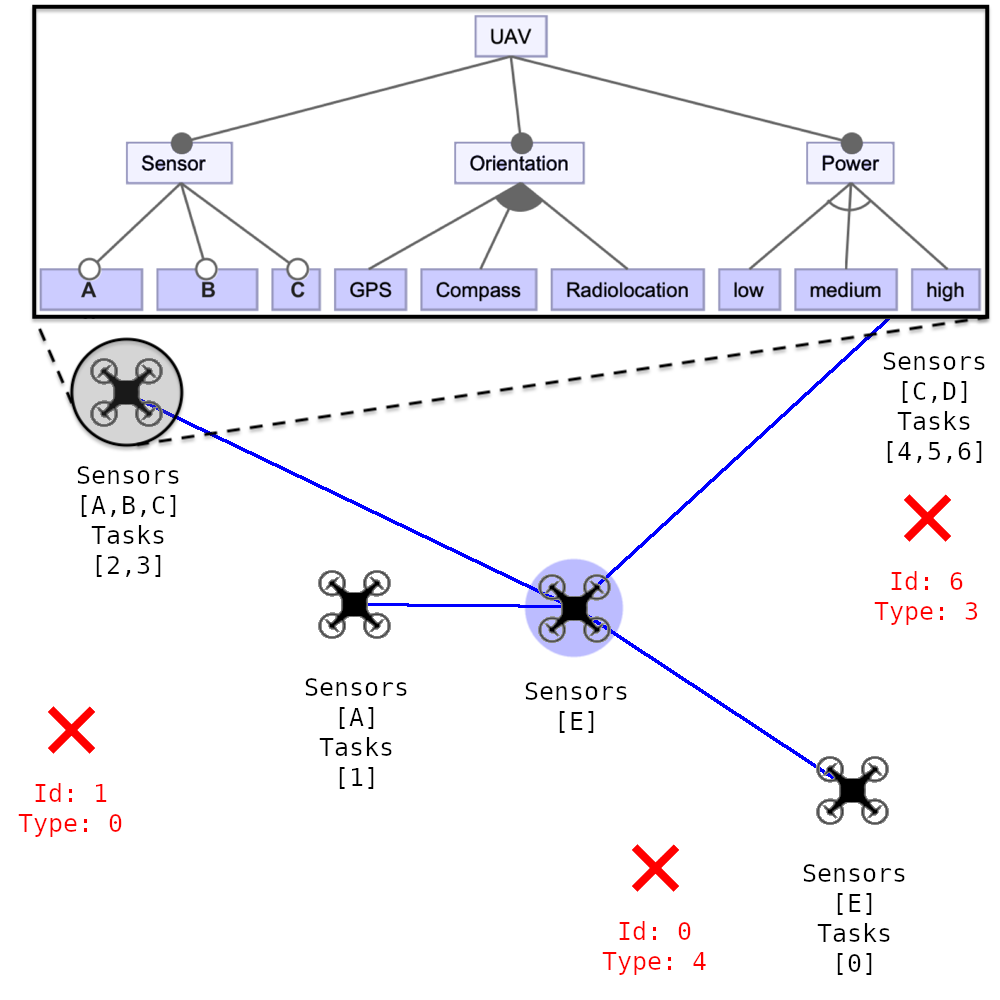
\includegraphics[width=0.95\linewidth]{img/scenario_01.png}
	    \caption{Feature Model showing UAV internal structure\label{fig:scene01}}
	\end{subfigure}
	\begin{subfigure}[t]{.45\textwidth}
	\centering
	    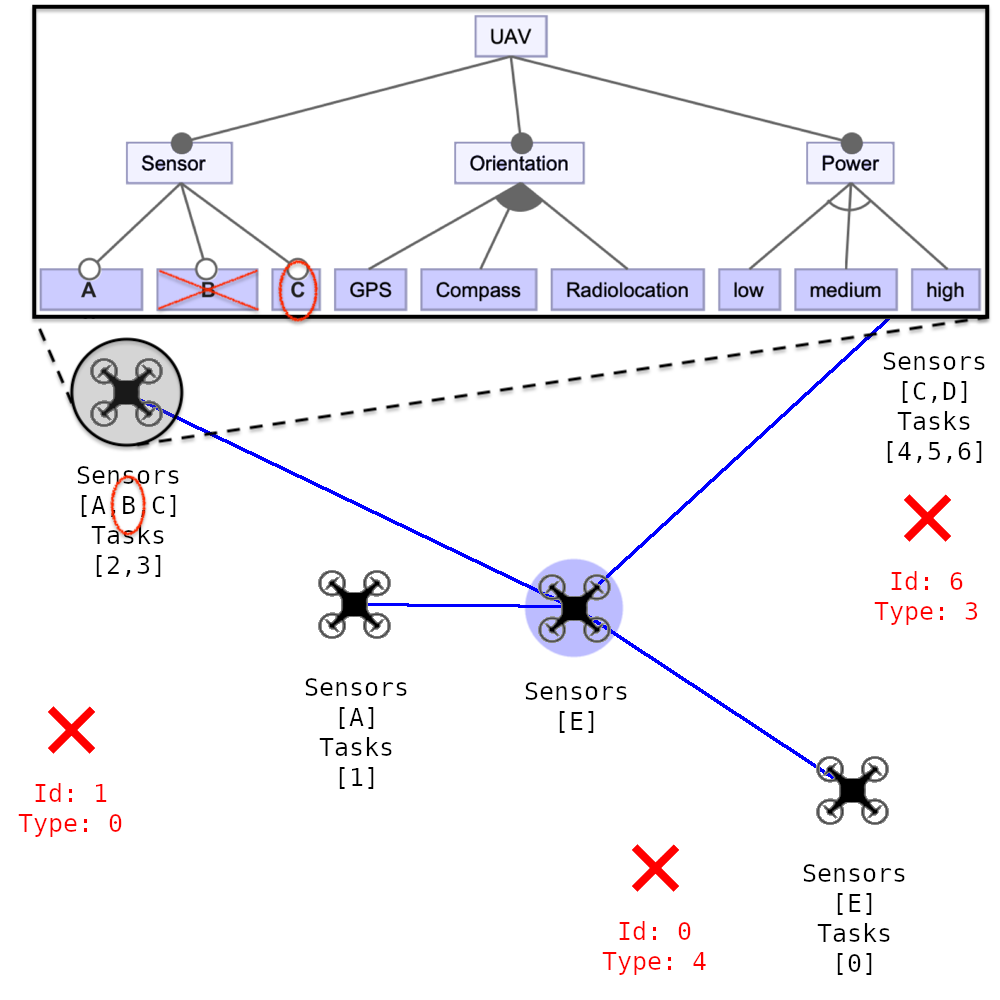
\includegraphics[width=0.95\linewidth]{img/scenario_02.png}
	    \caption{Feature activation to deal with context change\label{fig:scene02}}
	\end{subfigure}
	\caption{Member modeling using a Feature Model (partial view)indicating a reconfiguration performed by the TP, deactivating the feature related to sensor B and activating sensor C}
	\label{fig:TP_behavior}
\end{figure}

Based on this, a member $e$ is capable of executing a task $t$ when it reconfigures itself to adopt a configuration $c \in [\![FM]\!]$ such that this configuration makes the member capable of dealing with the task $t$.  This compatibility is known at the start and is denoted by $compatible(c, t)$. This configuration is characterized by sensors activated. There is a score, between 0 and 1, which indicates the compatibility level between each sensor $i$ onboard and the type of a task $j$, written as $Q_{ij}$ and so named quality. In summary, a member can receive a task $j$ when it has a sensor $i$ enabled whose $Q_{ij}$ meets the threshold, i.e., the acceptance level defined.  

%\begin{equation}
%    \label{eq:prop6}
%    compatible(e, t) \iff \exists c \in C_e \ \bullet compatible(c, t)
%\end{equation}

Figure~\ref{fig:ex_pg} defines \X{TP} behavior formally. Accordingly, upon mission start (guard $g_0$), TP has an initial configuration $c_0$, i.e., initial state defined by \X{members'} characteristics or even by the domain requirements, and an initial C2 strategy $w_0$ received through channel $ch2$ from $C2AM$ (location \textit{Idle}). An example of initial configuration is an energy safe mode, i.e., all sensors off, operated \X{to increase members' operating range}.

\begin{figure}[ht!]
    \centering
    \scalebox{.75}{

\tikzset{every picture/.style={line width=0.75pt}} %set default line width to 0.75pt        

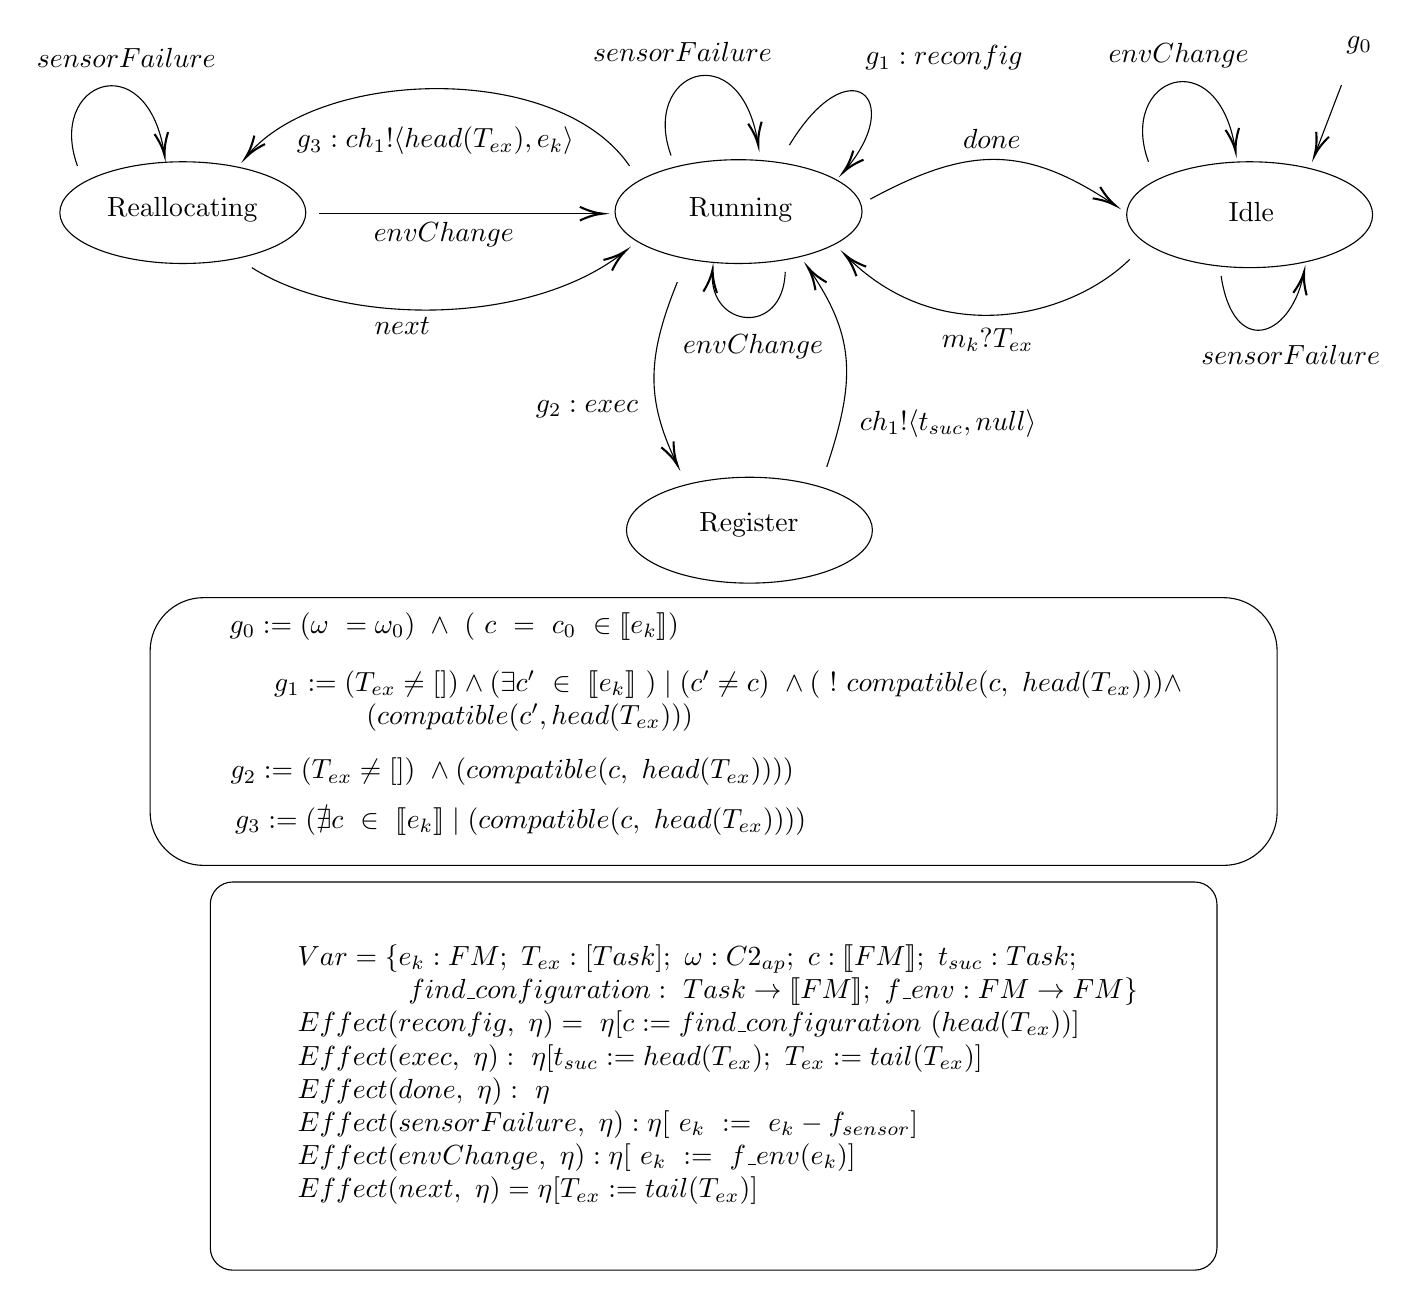
\begin{tikzpicture}[x=0.75pt,y=0.75pt,yscale=-1,xscale=1]
%uncomment if require: \path (0,620); %set diagram left start at 0, and has height of 620

%Curve Lines [id:da9480858267519683] 
\draw    (385.5,222) .. controls (399.29,180.63) and (399.5,159.63) .. (377.52,127.48) ;
\draw [shift={(376.5,126)}, rotate = 415.12] [color={rgb, 255:red, 0; green, 0; blue, 0 }  ][line width=0.75]    (10.93,-3.29) .. controls (6.95,-1.4) and (3.31,-0.3) .. (0,0) .. controls (3.31,0.3) and (6.95,1.4) .. (10.93,3.29)   ;
%Shape: Ellipse [id:dp6594609066072359] 
\draw   (283.5,99) .. controls (283.5,85.19) and (310.14,74) .. (343,74) .. controls (375.86,74) and (402.5,85.19) .. (402.5,99) .. controls (402.5,112.81) and (375.86,124) .. (343,124) .. controls (310.14,124) and (283.5,112.81) .. (283.5,99) -- cycle ;
%Shape: Ellipse [id:dp873836537729809] 
\draw   (530,100.5) .. controls (530,86.42) and (556.53,75) .. (589.25,75) .. controls (621.97,75) and (648.5,86.42) .. (648.5,100.5) .. controls (648.5,114.58) and (621.97,126) .. (589.25,126) .. controls (556.53,126) and (530,114.58) .. (530,100.5) -- cycle ;
%Curve Lines [id:da21020703050779688] 
\draw    (367.5,67) .. controls (396.21,19.48) and (423.94,44.49) .. (394.41,78.95) ;
\draw [shift={(393.5,80)}, rotate = 311.53] [color={rgb, 255:red, 0; green, 0; blue, 0 }  ][line width=0.75]    (10.93,-3.29) .. controls (6.95,-1.4) and (3.31,-0.3) .. (0,0) .. controls (3.31,0.3) and (6.95,1.4) .. (10.93,3.29)   ;
%Straight Lines [id:da37650774099478246] 
\draw    (633.5,38) -- (621.21,70.13) ;
\draw [shift={(620.5,72)}, rotate = 290.92] [color={rgb, 255:red, 0; green, 0; blue, 0 }  ][line width=0.75]    (10.93,-3.29) .. controls (6.95,-1.4) and (3.31,-0.3) .. (0,0) .. controls (3.31,0.3) and (6.95,1.4) .. (10.93,3.29)   ;
%Shape: Ellipse [id:dp02234558999259495] 
\draw   (16,99.5) .. controls (16,85.97) and (42.53,75) .. (75.25,75) .. controls (107.97,75) and (134.5,85.97) .. (134.5,99.5) .. controls (134.5,113.03) and (107.97,124) .. (75.25,124) .. controls (42.53,124) and (16,113.03) .. (16,99.5) -- cycle ;
%Curve Lines [id:da2517277021570281] 
\draw    (290.5,77) .. controls (255.85,26.51) and (141.81,29.93) .. (106.54,71.72) ;
\draw [shift={(105.5,73)}, rotate = 308.33000000000004] [color={rgb, 255:red, 0; green, 0; blue, 0 }  ][line width=0.75]    (10.93,-3.29) .. controls (6.95,-1.4) and (3.31,-0.3) .. (0,0) .. controls (3.31,0.3) and (6.95,1.4) .. (10.93,3.29)   ;
%Curve Lines [id:da851947022127026] 
\draw    (108.5,126) .. controls (152.06,153.72) and (240.7,154.98) .. (287.11,119.1) ;
\draw [shift={(288.5,118)}, rotate = 501.19] [color={rgb, 255:red, 0; green, 0; blue, 0 }  ][line width=0.75]    (10.93,-3.29) .. controls (6.95,-1.4) and (3.31,-0.3) .. (0,0) .. controls (3.31,0.3) and (6.95,1.4) .. (10.93,3.29)   ;
%Curve Lines [id:da05773774536505705] 
\draw    (531.5,122) .. controls (503.29,149.72) and (440.77,165.68) .. (395.86,121.36) ;
\draw [shift={(394.5,120)}, rotate = 405.63] [color={rgb, 255:red, 0; green, 0; blue, 0 }  ][line width=0.75]    (10.93,-3.29) .. controls (6.95,-1.4) and (3.31,-0.3) .. (0,0) .. controls (3.31,0.3) and (6.95,1.4) .. (10.93,3.29)   ;
%Rounded Rect [id:dp5913972444482631] 
\draw   (59.5,310.8) .. controls (59.5,296.55) and (71.05,285) .. (85.3,285) -- (576.7,285) .. controls (590.95,285) and (602.5,296.55) .. (602.5,310.8) -- (602.5,388.2) .. controls (602.5,402.45) and (590.95,414) .. (576.7,414) -- (85.3,414) .. controls (71.05,414) and (59.5,402.45) .. (59.5,388.2) -- cycle ;
%Rounded Rect [id:dp9206164489184118] 
\draw   (88.5,432.74) .. controls (88.5,426.81) and (93.31,422) .. (99.24,422) -- (562.76,422) .. controls (568.69,422) and (573.5,426.81) .. (573.5,432.74) -- (573.5,598.26) .. controls (573.5,604.19) and (568.69,609) .. (562.76,609) -- (99.24,609) .. controls (93.31,609) and (88.5,604.19) .. (88.5,598.26) -- cycle ;
%Curve Lines [id:da46585089178877326] 
\draw    (24.5,77) .. controls (9.65,36.41) and (57.53,18.36) .. (66.25,70.4) ;
\draw [shift={(66.5,72)}, rotate = 261.57] [color={rgb, 255:red, 0; green, 0; blue, 0 }  ][line width=0.75]    (10.93,-3.29) .. controls (6.95,-1.4) and (3.31,-0.3) .. (0,0) .. controls (3.31,0.3) and (6.95,1.4) .. (10.93,3.29)   ;
%Curve Lines [id:da24525569786800605] 
\draw    (575.5,130) .. controls (581.38,169.2) and (608.39,160.38) .. (615.11,129.89) ;
\draw [shift={(615.5,128)}, rotate = 460.62] [color={rgb, 255:red, 0; green, 0; blue, 0 }  ][line width=0.75]    (10.93,-3.29) .. controls (6.95,-1.4) and (3.31,-0.3) .. (0,0) .. controls (3.31,0.3) and (6.95,1.4) .. (10.93,3.29)   ;
%Curve Lines [id:da5617910694928671] 
\draw    (310.5,72) .. controls (295.65,31.41) and (343.53,13.36) .. (352.25,65.4) ;
\draw [shift={(352.5,67)}, rotate = 261.57] [color={rgb, 255:red, 0; green, 0; blue, 0 }  ][line width=0.75]    (10.93,-3.29) .. controls (6.95,-1.4) and (3.31,-0.3) .. (0,0) .. controls (3.31,0.3) and (6.95,1.4) .. (10.93,3.29)   ;
%Shape: Ellipse [id:dp893416141673501] 
\draw   (289,252.5) .. controls (289,238.42) and (315.53,227) .. (348.25,227) .. controls (380.97,227) and (407.5,238.42) .. (407.5,252.5) .. controls (407.5,266.58) and (380.97,278) .. (348.25,278) .. controls (315.53,278) and (289,266.58) .. (289,252.5) -- cycle ;
%Curve Lines [id:da2982425830385871] 
\draw    (313.5,133) .. controls (298.72,169.45) and (298.5,189.4) .. (312.84,219.61) ;
\draw [shift={(313.5,221)}, rotate = 244.18] [color={rgb, 255:red, 0; green, 0; blue, 0 }  ][line width=0.75]    (10.93,-3.29) .. controls (6.95,-1.4) and (3.31,-0.3) .. (0,0) .. controls (3.31,0.3) and (6.95,1.4) .. (10.93,3.29)   ;
%Curve Lines [id:da08998093824564413] 
\draw    (406.5,93) .. controls (454.02,67.26) and (480.96,67) .. (523.21,95.14) ;
\draw [shift={(524.5,96)}, rotate = 214] [color={rgb, 255:red, 0; green, 0; blue, 0 }  ][line width=0.75]    (10.93,-3.29) .. controls (6.95,-1.4) and (3.31,-0.3) .. (0,0) .. controls (3.31,0.3) and (6.95,1.4) .. (10.93,3.29)   ;
%Curve Lines [id:da7980176061132549] 
\draw    (365.5,128) .. controls (364.52,159.36) and (328.97,155.19) .. (330.37,128.65) ;
\draw [shift={(330.5,127)}, rotate = 456.12] [color={rgb, 255:red, 0; green, 0; blue, 0 }  ][line width=0.75]    (10.93,-3.29) .. controls (6.95,-1.4) and (3.31,-0.3) .. (0,0) .. controls (3.31,0.3) and (6.95,1.4) .. (10.93,3.29)   ;
%Curve Lines [id:da863076595467461] 
\draw    (540.5,75) .. controls (525.65,34.41) and (573.53,16.36) .. (582.25,68.4) ;
\draw [shift={(582.5,70)}, rotate = 261.57] [color={rgb, 255:red, 0; green, 0; blue, 0 }  ][line width=0.75]    (10.93,-3.29) .. controls (6.95,-1.4) and (3.31,-0.3) .. (0,0) .. controls (3.31,0.3) and (6.95,1.4) .. (10.93,3.29)   ;
%Straight Lines [id:da7258762513235244] 
\draw    (141,100) -- (275.5,100) ;
\draw [shift={(277.5,100)}, rotate = 180] [color={rgb, 255:red, 0; green, 0; blue, 0 }  ][line width=0.75]    (10.93,-3.29) .. controls (6.95,-1.4) and (3.31,-0.3) .. (0,0) .. controls (3.31,0.3) and (6.95,1.4) .. (10.93,3.29)   ;

% Text Node
\draw (344,98) node   [align=left] {Running};
% Text Node
\draw (590,99) node   [align=left] {Idle};
% Text Node
\draw (197,65) node    {$g_{3} :ch_{1} !\langle head( T_{ex}) ,e_{k} \rangle $};
% Text Node
\draw (463,161) node    {$m_{k} ?T_{ex}$};
% Text Node
\draw (75,98) node   [align=left] {Reallocating};
% Text Node
\draw (181,154) node    {$next$};
% Text Node
\draw (338,335) node    {$ \begin{array}{l}
g_{1} :=( T_{ex} \neq []) \land ( \exists c'\ \in \ \llbracket e_{k} \rrbracket \ ) \mid ( c'\neq c) \ \land ( \ !\ compatible( c,\ head( T_{ex}))) \land \\
\ \ \ \ \ \ \ \ \ \ ( compatible( c',head( T_{ex})))
\end{array}$};
% Text Node
\draw (442,25) node    {$g_{1} :reconfig$};
% Text Node
\draw (270,194) node    {$g_{2} :exec$};
% Text Node
\draw (234,369) node    {$g_{2} :=( T_{ex} \neq []) \ \land ( compatible( c,\ head( T_{ex}))))$};
% Text Node
\draw (232,472) node    {$ \begin{array}{l}
\end{array}$};
% Text Node
\draw (333,515) node    {$ \begin{array}{l}
Var=\{e_{k} :FM;\ T_{ex} :[ Task] ;\ \omega :C2_{ap} ;\ c:\llbracket FM\rrbracket ;\ t_{suc} :Task;\ \\
\ \ \ \ \ \ \ \ \ \ \ \ find\_configuration:\ Task\rightarrow \llbracket FM\rrbracket ;\ f\_env:FM\rightarrow FM\}\\
Effect( reconfig,\ \eta ) =\ \eta [ c:=find\_configuration\ ( head( T_{ex}))]\\
Effect( exec,\ \eta ) :\ \eta [ t_{suc} :=head( T_{ex}) ;\ T_{ex} :=tail( T_{ex})]\\
Effect( done,\ \eta ) :\ \eta \\
Effect( sensorFailure,\ \eta ) :\eta [ \ e_{k} \ :=\ e_{k} -f_{sensor}]\\
Effect( envChange,\ \eta ) :\eta [ \ e_{k} \ :=\ f\_env( e_{k})]\\
Effect( next,\ \eta ) =\eta [ T_{ex} :=tail( T_{ex})]
\end{array}$};
% Text Node
\draw (642,19) node    {$g_{0}$};
% Text Node
\draw (238,393) node    {$g_{3} :=( \nexists c\ \in \ \llbracket e_{k} \rrbracket \mid ( compatible( c,\ head( T_{ex}))))$};
% Text Node
\draw (206,299) node    {$g_{0} :=( \omega \ =\omega _{0}) \ \land \ ( \ c\ =\ c_{0} \ \in \llbracket e_{k} \rrbracket )$};
% Text Node
\draw (48,25) node    {$sensorFailure$};
% Text Node
\draw (609,168) node    {$sensorFailure$};
% Text Node
\draw (465,64) node    {$done$};
% Text Node
\draw (316,22) node    {$sensorFailure$};
% Text Node
\draw (348,250) node   [align=left] {Register};
% Text Node
\draw (444,201) node    {$ch_{1} !\langle t_{suc} ,null\rangle $};
% Text Node
\draw (201,110) node    {$envChange$};
% Text Node
\draw (350,164) node    {$envChange$};
% Text Node
\draw (555,24) node    {$envChange$};


\end{tikzpicture}}
    \caption{Program Graph defining the Task Performer $k$ (TP) role}
    \label{fig:ex_pg}
\end{figure}

After the initial guard condition $g_0$ is satisfied and the first location is reached, as shown in~Figure~\ref{fig:ex_pg}, TP can eventually be allocated tasks $T_{ex}$ that arrive over its dedicated asynchronous channel $m_k$ with the TA, at which point it will start addressing these in sequence (location \textit{Running}). If TP is able to execute the first allocated task (guard $g_2$), it indicates successful task execution with the $exec$ action, moving to location $Register$, and reports such task to the TA over the shared asynchronous channel $ch_1$, then moving back to location \textit{Running}. If the member still has a configuration capable of addressing the task (guard $g_1$), it will reconfigure to it. Otherwise (guard $g_3$), it will notify this problematic task to the TA (location \textit{Reallocating}) and continue execution (location \textit{Running}). 

Alternatively, the member may non-deterministically experience sensor failure (action $sensorFailure$), whose effect is described by removing configurations with the corresponding feature from the member's feature model, i.e., a self-reconfiguration that can be improved by a task reallocation. This action together with members loss (action $memberFailure$) composes changes in the self. In such a case, the tasks can be reallocated or a new C2 Approach can be operated to improve the system's awareness about the situation.

\X{
In summary, the member's implementation as DSPL provides the first level for dealing with context changes. Figure~\ref{fig:dspl_approach} shows the DSPL approach steps performed by the~\emph{Task Performer} PG. The \emph{FM}, which models the DSPL, maps all sensors and other resources onboard in the UAV that can be activated or deactivated according to the required features, addressing all existing constraints between them. This mapping is oriented to maximize the quality and mission results, as described earlier.
}

\begin{figure}[ht]
    \centering
    \color{\highlight}
    \captionsetup{font={color=\highlight}}
    \scalebox{.75}{

\tikzset{every picture/.style={line width=0.75pt}} %set default line width to 0.75pt        

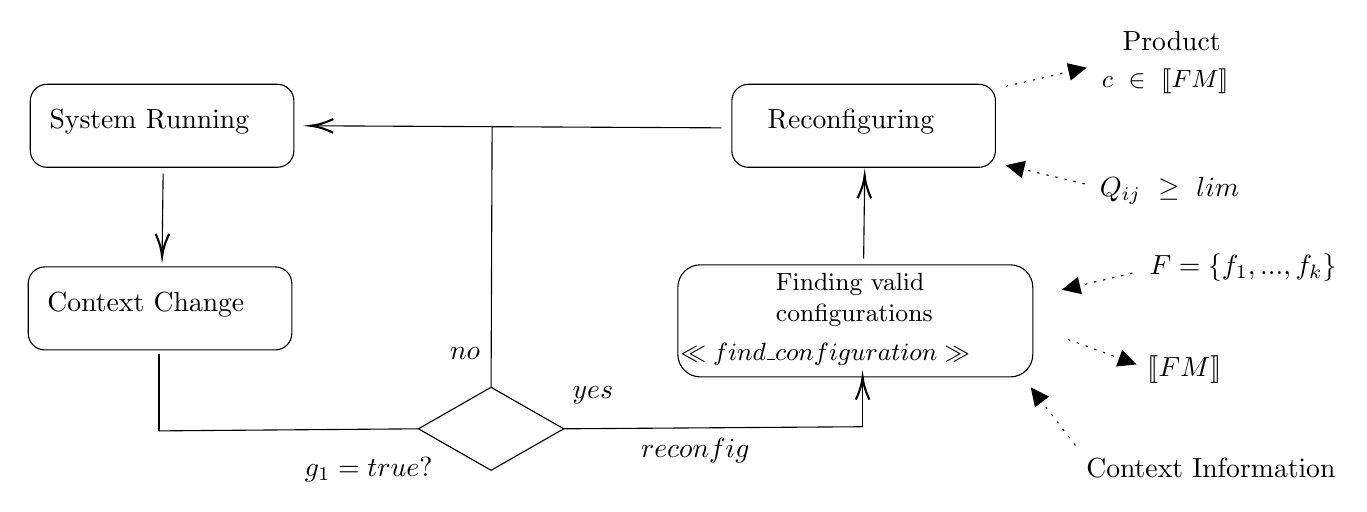
\begin{tikzpicture}[x=0.75pt,y=0.75pt,yscale=-1,xscale=1]
%uncomment if require: \path (0,244); %set diagram left start at 0, and has height of 244

%Rounded Rect [id:dp8066480632996035] 
\draw   (9,40) .. controls (9,35.58) and (12.58,32) .. (17,32) -- (128,32) .. controls (132.42,32) and (136,35.58) .. (136,40) -- (136,64) .. controls (136,68.42) and (132.42,72) .. (128,72) -- (17,72) .. controls (12.58,72) and (9,68.42) .. (9,64) -- cycle ;
%Rounded Rect [id:dp09986312472167136] 
\draw   (8,128) .. controls (8,123.58) and (11.58,120) .. (16,120) -- (127,120) .. controls (131.42,120) and (135,123.58) .. (135,128) -- (135,152) .. controls (135,156.42) and (131.42,160) .. (127,160) -- (16,160) .. controls (11.58,160) and (8,156.42) .. (8,152) -- cycle ;
%Rounded Rect [id:dp3203334247066908] 
\draw   (321,129.8) .. controls (321,123.84) and (325.84,119) .. (331.8,119) -- (481.2,119) .. controls (487.16,119) and (492,123.84) .. (492,129.8) -- (492,162.2) .. controls (492,168.16) and (487.16,173) .. (481.2,173) -- (331.8,173) .. controls (325.84,173) and (321,168.16) .. (321,162.2) -- cycle ;
%Straight Lines [id:da7215475210798592] 
\draw    (342,53) -- (146,52.01) ;
\draw [shift={(144,52)}, rotate = 0.29] [color={rgb, 255:red, 0; green, 0; blue, 0 }  ][line width=0.75]    (10.93,-3.29) .. controls (6.95,-1.4) and (3.31,-0.3) .. (0,0) .. controls (3.31,0.3) and (6.95,1.4) .. (10.93,3.29)   ;
%Straight Lines [id:da566488552820097] 
\draw    (73,75) -- (72.52,113) ;
\draw [shift={(72.5,115)}, rotate = 270.72] [color={rgb, 255:red, 0; green, 0; blue, 0 }  ][line width=0.75]    (10.93,-3.29) .. controls (6.95,-1.4) and (3.31,-0.3) .. (0,0) .. controls (3.31,0.3) and (6.95,1.4) .. (10.93,3.29)   ;
%Straight Lines [id:da03600720187770856] 
\draw  [dash pattern={on 0.84pt off 2.51pt}]  (509,155) -- (539.18,165.97) ;
\draw [shift={(542,167)}, rotate = 199.98] [fill={rgb, 255:red, 0; green, 0; blue, 0 }  ][line width=0.08]  [draw opacity=0] (8.93,-4.29) -- (0,0) -- (8.93,4.29) -- cycle    ;
%Rounded Rect [id:dp7101206593267378] 
\draw   (347,40) .. controls (347,35.58) and (350.58,32) .. (355,32) -- (466,32) .. controls (470.42,32) and (474,35.58) .. (474,40) -- (474,64) .. controls (474,68.42) and (470.42,72) .. (466,72) -- (355,72) .. controls (350.58,72) and (347,68.42) .. (347,64) -- cycle ;
%Straight Lines [id:da7286524767507477] 
\draw    (266,198) -- (410,197) ;
%Straight Lines [id:da695602580560019] 
\draw    (71,162) -- (71,199) ;
%Straight Lines [id:da47123812289807143] 
\draw    (410,175) -- (410,197) ;
\draw [shift={(410,173)}, rotate = 90] [color={rgb, 255:red, 0; green, 0; blue, 0 }  ][line width=0.75]    (10.93,-3.29) .. controls (6.95,-1.4) and (3.31,-0.3) .. (0,0) .. controls (3.31,0.3) and (6.95,1.4) .. (10.93,3.29)   ;
%Straight Lines [id:da7842612276994353] 
\draw  [dash pattern={on 0.84pt off 2.51pt}]  (517,80) -- (481.92,71.69) ;
\draw [shift={(479,71)}, rotate = 13.32] [fill={rgb, 255:red, 0; green, 0; blue, 0 }  ][line width=0.08]  [draw opacity=0] (8.93,-4.29) -- (0,0) -- (8.93,4.29) -- cycle    ;
%Straight Lines [id:da6842594623348534] 
\draw  [dash pattern={on 0.84pt off 2.51pt}]  (479,33) -- (515.08,24.67) ;
\draw [shift={(518,24)}, rotate = 167.01] [fill={rgb, 255:red, 0; green, 0; blue, 0 }  ][line width=0.08]  [draw opacity=0] (8.93,-4.29) -- (0,0) -- (8.93,4.29) -- cycle    ;
%Straight Lines [id:da2973367810568732] 
\draw    (410.98,78) -- (410.5,116) ;
\draw [shift={(411,76)}, rotate = 90.72] [color={rgb, 255:red, 0; green, 0; blue, 0 }  ][line width=0.75]    (10.93,-3.29) .. controls (6.95,-1.4) and (3.31,-0.3) .. (0,0) .. controls (3.31,0.3) and (6.95,1.4) .. (10.93,3.29)   ;
%Straight Lines [id:da9420001435559124] 
\draw  [dash pattern={on 0.84pt off 2.51pt}]  (540,123) -- (508.92,130.31) ;
\draw [shift={(506,131)}, rotate = 346.76] [fill={rgb, 255:red, 0; green, 0; blue, 0 }  ][line width=0.08]  [draw opacity=0] (8.93,-4.29) -- (0,0) -- (8.93,4.29) -- cycle    ;
%Flowchart: Decision [id:dp759598130534352] 
\draw   (231,178) -- (266,198) -- (231,218) -- (196,198) -- cycle ;
%Straight Lines [id:da367734053399414] 
\draw    (71,199) -- (196,198) ;
%Straight Lines [id:da5755851308332511] 
\draw    (231.5,52) -- (231,178) ;
%Straight Lines [id:da3242394337958049] 
\draw  [dash pattern={on 0.84pt off 2.51pt}]  (512.5,206) -- (492.83,180.38) ;
\draw [shift={(491,178)}, rotate = 52.48] [fill={rgb, 255:red, 0; green, 0; blue, 0 }  ][line width=0.08]  [draw opacity=0] (8.93,-4.29) -- (0,0) -- (8.93,4.29) -- cycle    ;

% Text Node
\draw (17,43) node [anchor=north west][inner sep=0.75pt]   [align=left] {System Running};
% Text Node
\draw (16,131) node [anchor=north west][inner sep=0.75pt]   [align=left] {Context Change};
% Text Node
\draw (367,122) node [anchor=north west][inner sep=0.75pt]  [font=\small] [align=left] {Finding valid\\configurations};
% Text Node
\draw (321,155.4) node [anchor=north west][inner sep=0.75pt]  [font=\small]  {$\ll find\_configuration\gg $};
% Text Node
\draw (546,161.4) node [anchor=north west][inner sep=0.75pt]    {$\llbracket FM\rrbracket $};
% Text Node
\draw (363,43) node [anchor=north west][inner sep=0.75pt]   [align=left] {Reconfiguring};
% Text Node
\draw (523,75.4) node [anchor=north west][inner sep=0.75pt]    {$Q_{ij} \ \geq \ lim$};
% Text Node
\draw (302,201.4) node [anchor=north west][inner sep=0.75pt]    {$reconfig$};
% Text Node
\draw (529,5) node [anchor=north west][inner sep=0.75pt]   [align=left] {\begin{minipage}[lt]{42.88pt}\setlength\topsep{0pt}
\begin{center}
Product
\end{center}

\end{minipage}};
% Text Node
\draw (547,112.4) node [anchor=north west][inner sep=0.75pt]    {$F=\{f_{1} ,...,f_{k}\}$};
% Text Node
\draw (524,23.4) node [anchor=north west][inner sep=0.75pt]  [font=\small]  {$c\ \in \ \llbracket FM\rrbracket $};
% Text Node
\draw (140,210.4) node [anchor=north west][inner sep=0.75pt]    {$g_{1} = true ?$};
% Text Node
\draw (269,176.4) node [anchor=north west][inner sep=0.75pt]    {$yes$};
% Text Node
\draw (210,157.4) node [anchor=north west][inner sep=0.75pt]    {$no$};
% Text Node
\draw (516.5,211) node [anchor=north west][inner sep=0.75pt]   [align=left] {Context Information};


\end{tikzpicture}}
    \caption{Task Performer actions related to the DSPL approach}
    \label{fig:dspl_approach}
\end{figure}

\X{
Any perturbation described in Section~\ref{sec:example} that makes the member’s configuration incompatible with the circumstance, i.e., guard condition $g_1$ equals to true, activates the action~\emph{reconfig}, that provides features activation according to tasks requirement. Algorithm~\ref{algo:reconfig_algo} describes the function~\emph{find\_configuration} that implements this action, which starts operating on the set of features $F$ to analyze their current status, and to generate an updated set of valid configurations $\llbracket FM \rrbracket$ compatible with the new circumstance (line~\ref{line:get_fm}). In addition, this reconfiguration may use information from the context, e.g., tasks allocation between other members in the team. 
}

\begin{algorithm}[h!t]
    \SetAlCapNameFnt{\small\color{\highlight}}
    \SetAlCapFnt{\small\color{\highlight}}
	\caption{Function $find\_configuration$ implementing the the $reconfig$ action to deal with new circumstance}
	\label{algo:reconfig_algo}
	
	\color{\highlight}
	\SetAlgoLined
	\DontPrintSemicolon
	\SetKwBlock{Loop}{loop}{end loop}
	\SetKwFor{ForAll}{for all}{do}{end for}
	
	%\SetAlgoNlRelativeSize{-3}
	\SetNlSty{text}{}{:}
	\SetNlSkip{0.3em}

    i := next task\;
    $\llbracket FM \rrbracket$ := valid configurations based on $F$\;\label{line:get_fm}
    \ForAll{ onboard sensor j }{\label{line:select_sensor_begin}
     $Q_{ij}$ = calculate quality to sensor $j$ be used in task $i$\;\label{line:calculate_quality}
     \If{($Q_{ij} \geq$ threshold)  $\land$  ($Q_{ij} >$ quality)}{quality = $Q_{ij}$\;\label{line:update_quality}
     selected\_sensor = j\;\label{line:select_sensor_end}}
    }
    select $c \in \llbracket FM \rrbracket \mid ( feature_{selected\_sensor} \in c$)\;\label{line:select_c}
    \ForAll{feature $f \in F$}{\label{line:select_f_begin}
    \If{$f \in c$}{activate $f$}
    \Else{deactivate $f$}\label{line:select_f_end}
    }
\end{algorithm}

\X{
Next, we perform a quality comparison of task $i$ and each sensor $j$, according to their compatibility. The reconfiguration selects the best configuration $c$ to satisfy required quality parameter, i.e., \emph{threshold} (lines~\ref{line:select_sensor_begin} --~\ref{line:select_sensor_end}). After this analysis, we select the most suitable configuration $c$ that contains only the required sensor $j$ activated (line~\ref{line:select_c}). In such a case, all other sensor are disabled (lines~\ref{line:select_f_begin} --~\ref{line:select_f_end}).
}




\subsubsection{Task Allocator}

In contrast to role TP, which focuses on task execution and member reconfiguration, TA defines coordination behavior among members, establishing task allocation responsibilities, as shown formally in Figure~\ref{fig:ta_pg}. \X{The members with such a role perform the tasks allocation according to quality levels. In addition, they reallocate tasks because of context changes. Figure~\ref{fig:TA_behavior} shows a task reallocation because of sensor issue, aiming at keeping mission's quality level.}

\begin{figure}[ht!]
    \centering
    \scalebox{.75}{

\tikzset{every picture/.style={line width=0.75pt}} %set default line width to 0.75pt        

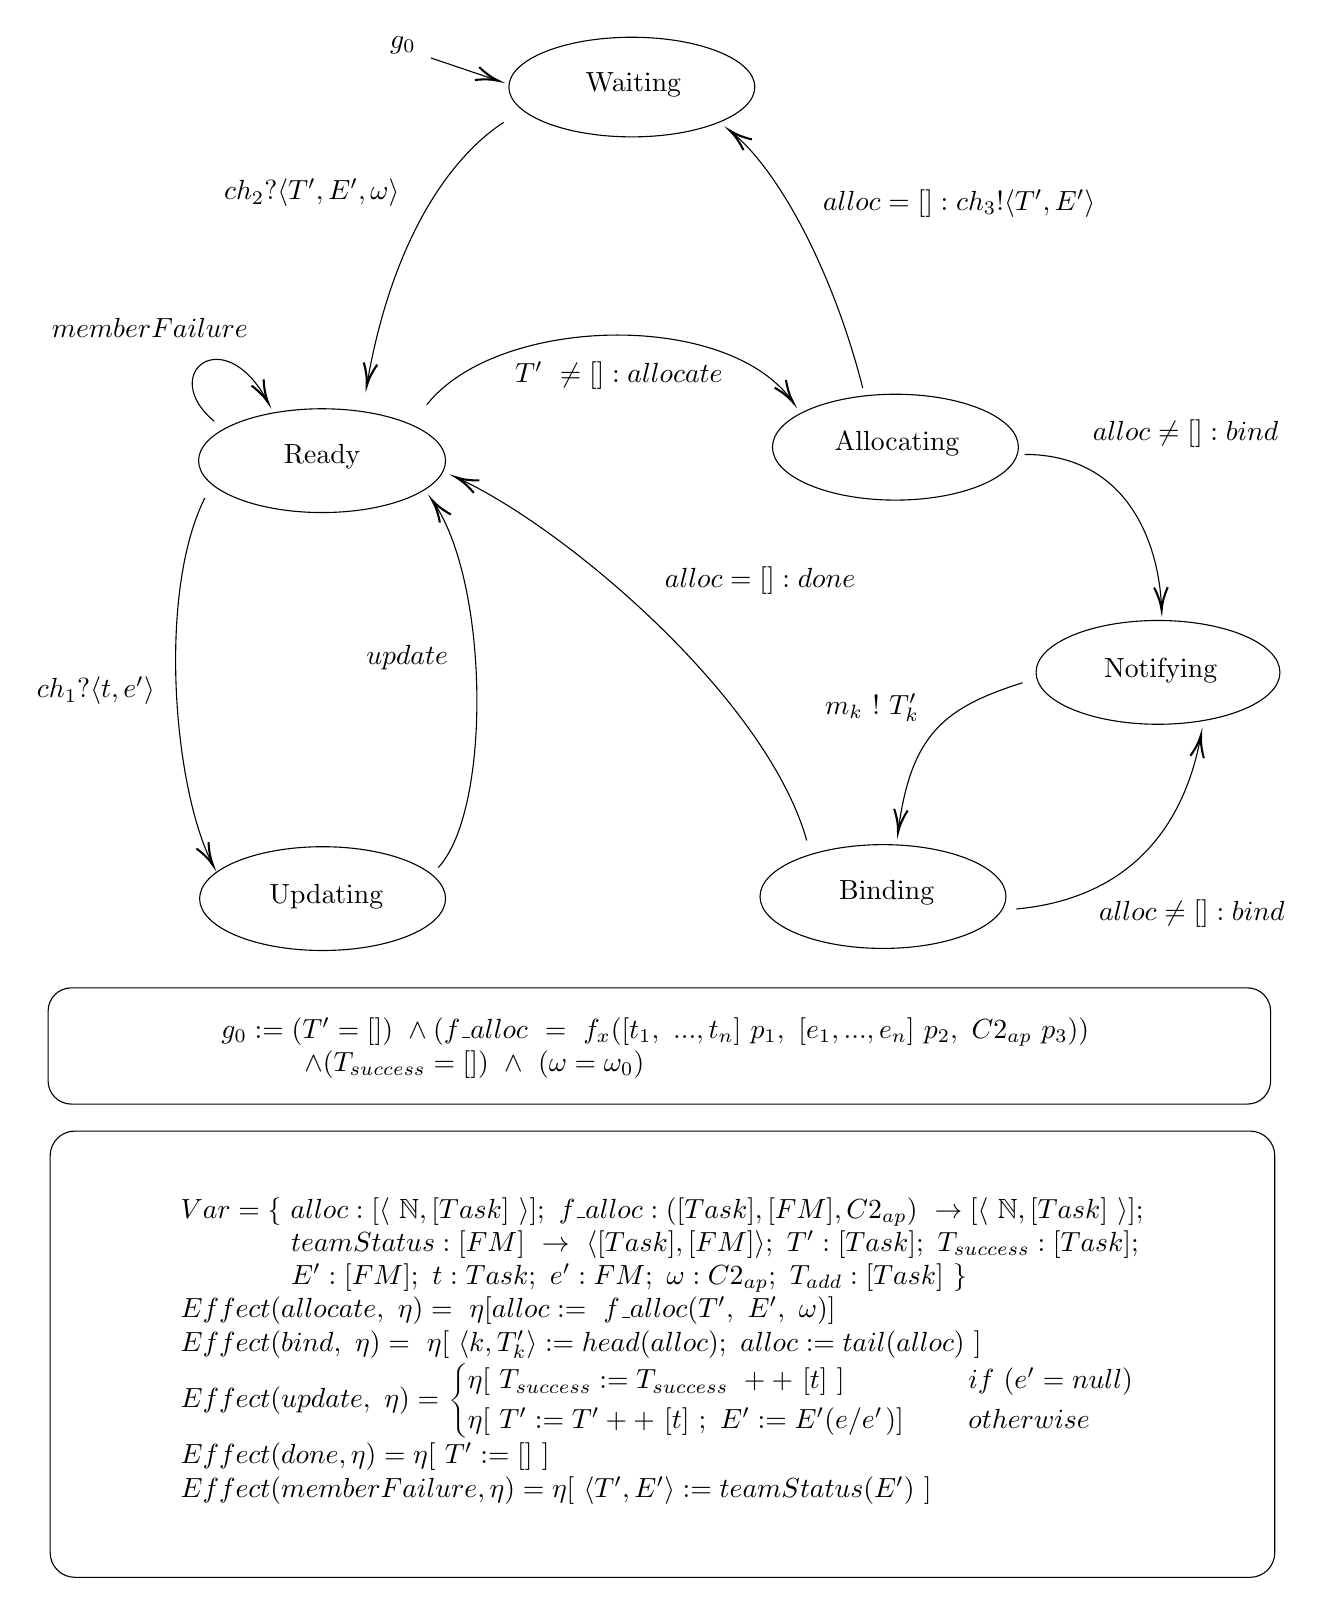
\begin{tikzpicture}[x=0.75pt,y=0.75pt,yscale=-1,xscale=1]
%uncomment if require: \path (0,763); %set diagram left start at 0, and has height of 763

%Curve Lines [id:da9480858267519683] 
\draw    (201.5,185) .. controls (235.16,142.43) and (344.78,139.06) .. (377.05,182.66) ;
\draw [shift={(378,184)}, rotate = 235.44] [color={rgb, 255:red, 0; green, 0; blue, 0 }  ][line width=0.75]    (10.93,-3.29) .. controls (6.95,-1.4) and (3.31,-0.3) .. (0,0) .. controls (3.31,0.3) and (6.95,1.4) .. (10.93,3.29)   ;
%Shape: Ellipse [id:dp6594609066072359] 
\draw   (91.5,212) .. controls (91.5,198.19) and (118.14,187) .. (151,187) .. controls (183.86,187) and (210.5,198.19) .. (210.5,212) .. controls (210.5,225.81) and (183.86,237) .. (151,237) .. controls (118.14,237) and (91.5,225.81) .. (91.5,212) -- cycle ;
%Shape: Ellipse [id:dp873836537729809] 
\draw   (368,205.5) .. controls (368,191.42) and (394.53,180) .. (427.25,180) .. controls (459.97,180) and (486.5,191.42) .. (486.5,205.5) .. controls (486.5,219.58) and (459.97,231) .. (427.25,231) .. controls (394.53,231) and (368,219.58) .. (368,205.5) -- cycle ;
%Curve Lines [id:da14662580418826565] 
\draw    (485.5,428) .. controls (538.96,423.05) and (565.96,389.68) .. (574.25,345.35) ;
\draw [shift={(574.5,344)}, rotate = 460.08] [color={rgb, 255:red, 0; green, 0; blue, 0 }  ][line width=0.75]    (10.93,-3.29) .. controls (6.95,-1.4) and (3.31,-0.3) .. (0,0) .. controls (3.31,0.3) and (6.95,1.4) .. (10.93,3.29)   ;
%Straight Lines [id:da37650774099478246] 
\draw    (203.5,18) -- (234.11,28.36) ;
\draw [shift={(236,29)}, rotate = 198.7] [color={rgb, 255:red, 0; green, 0; blue, 0 }  ][line width=0.75]    (10.93,-3.29) .. controls (6.95,-1.4) and (3.31,-0.3) .. (0,0) .. controls (3.31,0.3) and (6.95,1.4) .. (10.93,3.29)   ;
%Shape: Ellipse [id:dp8139093405894636] 
\draw   (92,423) .. controls (92,409.19) and (118.53,398) .. (151.25,398) .. controls (183.97,398) and (210.5,409.19) .. (210.5,423) .. controls (210.5,436.81) and (183.97,448) .. (151.25,448) .. controls (118.53,448) and (92,436.81) .. (92,423) -- cycle ;
%Shape: Ellipse [id:dp08678607998247811] 
\draw   (362,422) .. controls (362,408.19) and (388.53,397) .. (421.25,397) .. controls (453.97,397) and (480.5,408.19) .. (480.5,422) .. controls (480.5,435.81) and (453.97,447) .. (421.25,447) .. controls (388.53,447) and (362,435.81) .. (362,422) -- cycle ;
%Shape: Ellipse [id:dp07482494496489733] 
\draw   (241,32) .. controls (241,18.75) and (267.53,8) .. (300.25,8) .. controls (332.97,8) and (359.5,18.75) .. (359.5,32) .. controls (359.5,45.25) and (332.97,56) .. (300.25,56) .. controls (267.53,56) and (241,45.25) .. (241,32) -- cycle ;
%Curve Lines [id:da6759956440889884] 
\draw    (94.5,230) .. controls (71.84,275.31) and (79.27,368.16) .. (97.65,405.34) ;
\draw [shift={(98.5,407)}, rotate = 242.18] [color={rgb, 255:red, 0; green, 0; blue, 0 }  ][line width=0.75]    (10.93,-3.29) .. controls (6.95,-1.4) and (3.31,-0.3) .. (0,0) .. controls (3.31,0.3) and (6.95,1.4) .. (10.93,3.29)   ;
%Curve Lines [id:da9572857730465772] 
\draw    (205.22,232.76) .. controls (231.54,272.31) and (232.61,380.42) .. (207,408) ;
\draw [shift={(204,231)}, rotate = 54.11] [color={rgb, 255:red, 0; green, 0; blue, 0 }  ][line width=0.75]    (10.93,-3.29) .. controls (6.95,-1.4) and (3.31,-0.3) .. (0,0) .. controls (3.31,0.3) and (6.95,1.4) .. (10.93,3.29)   ;
%Curve Lines [id:da9385545433271328] 
\draw    (488.5,319) .. controls (450.88,330.88) and (434.82,343.74) .. (428.68,389.6) ;
\draw [shift={(428.5,391)}, rotate = 277.28] [color={rgb, 255:red, 0; green, 0; blue, 0 }  ][line width=0.75]    (10.93,-3.29) .. controls (6.95,-1.4) and (3.31,-0.3) .. (0,0) .. controls (3.31,0.3) and (6.95,1.4) .. (10.93,3.29)   ;
%Curve Lines [id:da13526468384837043] 
\draw    (411.5,177) .. controls (397.78,123.1) and (372.54,74) .. (348.94,54.18) ;
\draw [shift={(347.5,53)}, rotate = 398.37] [color={rgb, 255:red, 0; green, 0; blue, 0 }  ][line width=0.75]    (10.93,-3.29) .. controls (6.95,-1.4) and (3.31,-0.3) .. (0,0) .. controls (3.31,0.3) and (6.95,1.4) .. (10.93,3.29)   ;
%Curve Lines [id:da7876400787103589] 
\draw    (238.5,49) .. controls (209.79,67.81) and (184.02,110.14) .. (172.83,174.06) ;
\draw [shift={(172.5,176)}, rotate = 279.61] [color={rgb, 255:red, 0; green, 0; blue, 0 }  ][line width=0.75]    (10.93,-3.29) .. controls (6.95,-1.4) and (3.31,-0.3) .. (0,0) .. controls (3.31,0.3) and (6.95,1.4) .. (10.93,3.29)   ;
%Shape: Ellipse [id:dp538933115831977] 
\draw   (495,314) .. controls (495,300.19) and (521.3,289) .. (553.75,289) .. controls (586.2,289) and (612.5,300.19) .. (612.5,314) .. controls (612.5,327.81) and (586.2,339) .. (553.75,339) .. controls (521.3,339) and (495,327.81) .. (495,314) -- cycle ;
%Curve Lines [id:da663291454681702] 
\draw    (489.5,209) .. controls (537.52,209) and (553.85,249.34) .. (555.42,282.01) ;
\draw [shift={(555.5,284)}, rotate = 268.26] [color={rgb, 255:red, 0; green, 0; blue, 0 }  ][line width=0.75]    (10.93,-3.29) .. controls (6.95,-1.4) and (3.31,-0.3) .. (0,0) .. controls (3.31,0.3) and (6.95,1.4) .. (10.93,3.29)   ;
%Curve Lines [id:da17641910717404863] 
\draw    (384.5,395) .. controls (365.69,327.68) and (270.43,245.66) .. (217.1,220.74) ;
\draw [shift={(215.5,220)}, rotate = 384.36] [color={rgb, 255:red, 0; green, 0; blue, 0 }  ][line width=0.75]    (10.93,-3.29) .. controls (6.95,-1.4) and (3.31,-0.3) .. (0,0) .. controls (3.31,0.3) and (6.95,1.4) .. (10.93,3.29)   ;
%Rounded Rect [id:dp2887172897272543] 
\draw   (20,546.88) .. controls (20,540.32) and (25.32,535) .. (31.88,535) -- (598.12,535) .. controls (604.68,535) and (610,540.32) .. (610,546.88) -- (610,738.12) .. controls (610,744.68) and (604.68,750) .. (598.12,750) -- (31.88,750) .. controls (25.32,750) and (20,744.68) .. (20,738.12) -- cycle ;
%Rounded Rect [id:dp07131134126212679] 
\draw   (19,477.2) .. controls (19,471.01) and (24.01,466) .. (30.2,466) -- (596.8,466) .. controls (602.99,466) and (608,471.01) .. (608,477.2) -- (608,510.8) .. controls (608,516.99) and (602.99,522) .. (596.8,522) -- (30.2,522) .. controls (24.01,522) and (19,516.99) .. (19,510.8) -- cycle ;
%Curve Lines [id:da580151899278355] 
\draw    (99,193) .. controls (71.91,170.34) and (103.04,144.78) .. (124.05,182.24) ;
\draw [shift={(125,184)}, rotate = 242.3] [color={rgb, 255:red, 0; green, 0; blue, 0 }  ][line width=0.75]    (10.93,-3.29) .. controls (6.95,-1.4) and (3.31,-0.3) .. (0,0) .. controls (3.31,0.3) and (6.95,1.4) .. (10.93,3.29)   ;

% Text Node
\draw (151,210) node   [align=left] {Ready};
% Text Node
\draw (428,204) node   [align=left] {Allocating};
% Text Node
\draw (294,171) node    {$T'\ \neq [] :allocate$};
% Text Node
\draw (153,422) node   [align=left] {Updating};
% Text Node
\draw (555,313) node   [align=left] {Notifying};
% Text Node
\draw (301,31) node   [align=left] {Waiting};
% Text Node
\draw (42,323) node    {$ch_{1} ?\langle t,e' \rangle $};
% Text Node
\draw (192,307) node    {$update$};
% Text Node
\draw (458,88) node    {$alloc=[] :ch_{3} !\langle T',E'\rangle $};
% Text Node
\draw (146,83) node    {$ch_{2} ?\langle T',E',\omega \rangle $};
% Text Node
\draw (423,420) node   [align=left] {Binding};
% Text Node
\draw (570,430) node    {$alloc\neq [] :bind$};
% Text Node
\draw (416,331) node    {$m_{k\ } !\ T'_{k}$};
% Text Node
\draw (567,199) node    {$alloc\neq [] :bind$};
% Text Node
\draw (362,270) node    {$alloc=[] :done$};
% Text Node
\draw (317,641) node    {$ \begin{array}{l}
Var=\{\ alloc:[ \langle \ \mathbb{N} ,[ Task] \ \rangle ] ;\ f\_alloc:([ Task] ,[ FM] ,C2_{ap}) \ \rightarrow [ \langle \ \mathbb{N} ,[ Task] \ \rangle ] ;\ \\
\ \ \ \ \ \ \ \ \ \ \ \ teamStatus:[ FM] \ \rightarrow \ \langle [ Task] ,[ FM] \rangle ;\ T':[ Task] ;\ T_{success} :[ Task] ;\ \\
\ \ \ \ \ \ \ \ \ \ \ \ E':[ FM] ;\ t:Task;\ e' :FM;\ \omega :C2_{ap} ;\ T_{add} :[ Task] \ \}\\
Effect( allocate,\ \eta ) =\ \eta [ alloc:=\ f\_alloc( T',\ E',\ \omega )]\\
Effect( bind,\ \eta ) =\ \eta [ \ \langle k,T'_{k} \rangle :=head( alloc) ;\ alloc:=tail( alloc) \ ]\\
Effect( update,\ \eta ) =\begin{cases}
\eta [ \ T_{success} :=T_{success} \ ++\ [ t] \ ] & \ \ \ \ if\ ( e'=null)\\
\eta [ \ T':=T'++\ [ t] \ ;\ E':=E'( e/e'_{\ })] & \ \ \ \ otherwise
\end{cases} \ \\
Effect( done,\eta ) =\eta [ \ T':=[] \ ]\\
Effect( memberFailure,\eta ) =\eta [ \ \langle T',E'\rangle :=teamStatus( E') \ ]
\end{array}$};
% Text Node
\draw (190,12) node    {$g_{0}$};
% Text Node
\draw (313.76,495) node    {$ \begin{array}{l}
g_{0} :=( T'=[]) \ \land ( f\_alloc\ =\ f_{x}([ t_{1} ,\ ...,t_{n}] \ p_{1} ,\ [ e_{1} ,...,e_{n}] \ p_{2} ,\ C2_{ap} \ p_{3})) \ \\
\ \ \ \ \ \ \ \ \ \land ( T_{success} =[]) \ \land \ ( \omega =\omega _{0})
\end{array}$};
% Text Node
\draw (68,148) node    {$memberFailure$};


\end{tikzpicture}}
    \caption{Program Graph defining the Task Allocator (TA) role}
    \label{fig:ta_pg}
\end{figure}


When the mission starts, TA is in the \textit{Waiting} location, staying there until it receives mission tasks $T'$ and members information $E'$ from the C2AM over the synchronous channel $ch_2$, then moving to location $Ready$. TA then performs task allocation (action $allocate$),  notifies each member $k$ (locations \textit{Notifying} and \textit{Binding}) of its assigned task $T'_k$ via an specific asynchronous channel $m_k$, returning to the \textit{Ready} location. Eventually, TA will be notified, over a shared asynchronous channel $ch_1$, of successfully completed tasks by the members and of failed tasks, in which case it will perform a new task allocation. In case of members' failure (action $memberFailure$), the TA tries to reallocate tasks previously allocated to those members. If unsuccessful, the TA reports such tasks along with members' status to the C2AM over the synchronous channel $ch_3$. 

\begin{figure}[!htbp]
	\centering
	\captionsetup{font={color=\highlight}}
	\begin{subfigure}[t]{.45\textwidth}
	\centering
	    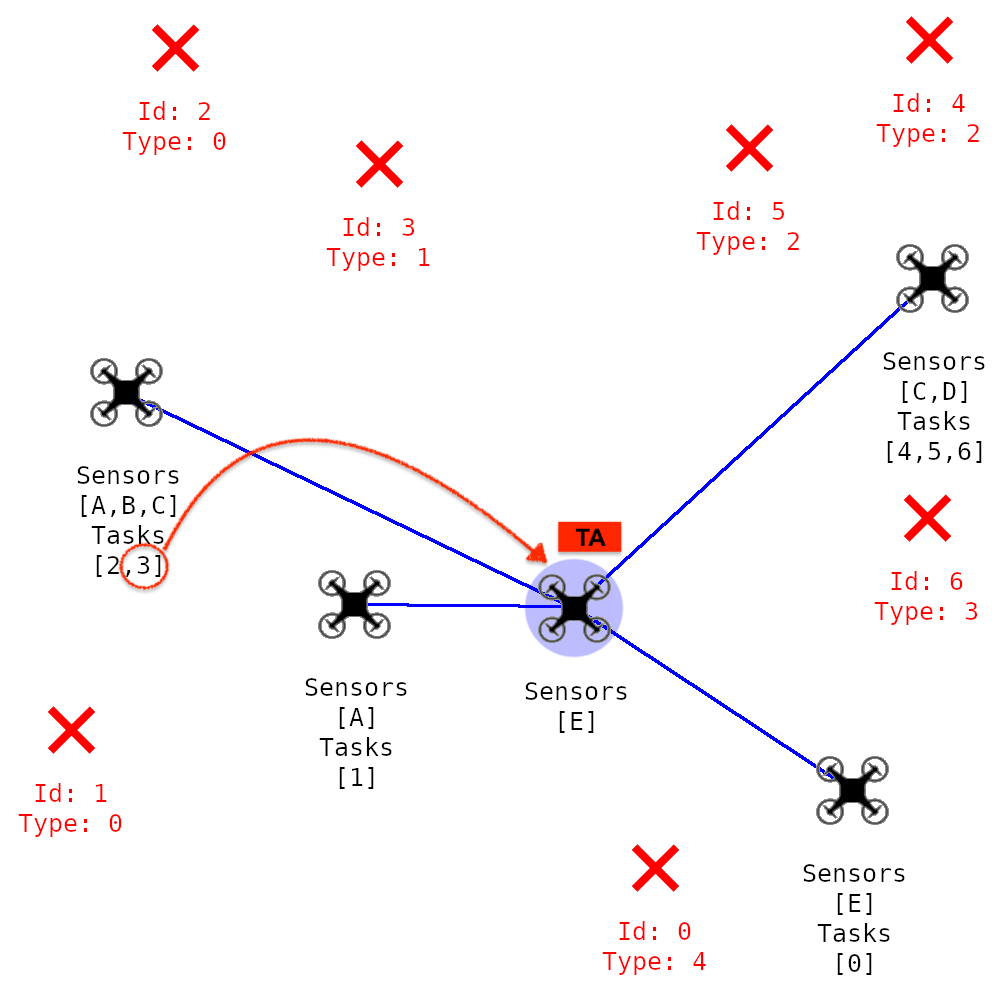
\includegraphics[width=0.95\linewidth]{img/scenario_03.png}
	    \caption{Member sends back a task not executable due to internal issues\label{fig:scene03}}
	\end{subfigure}
	\begin{subfigure}[t]{.45\textwidth}
	\centering
	    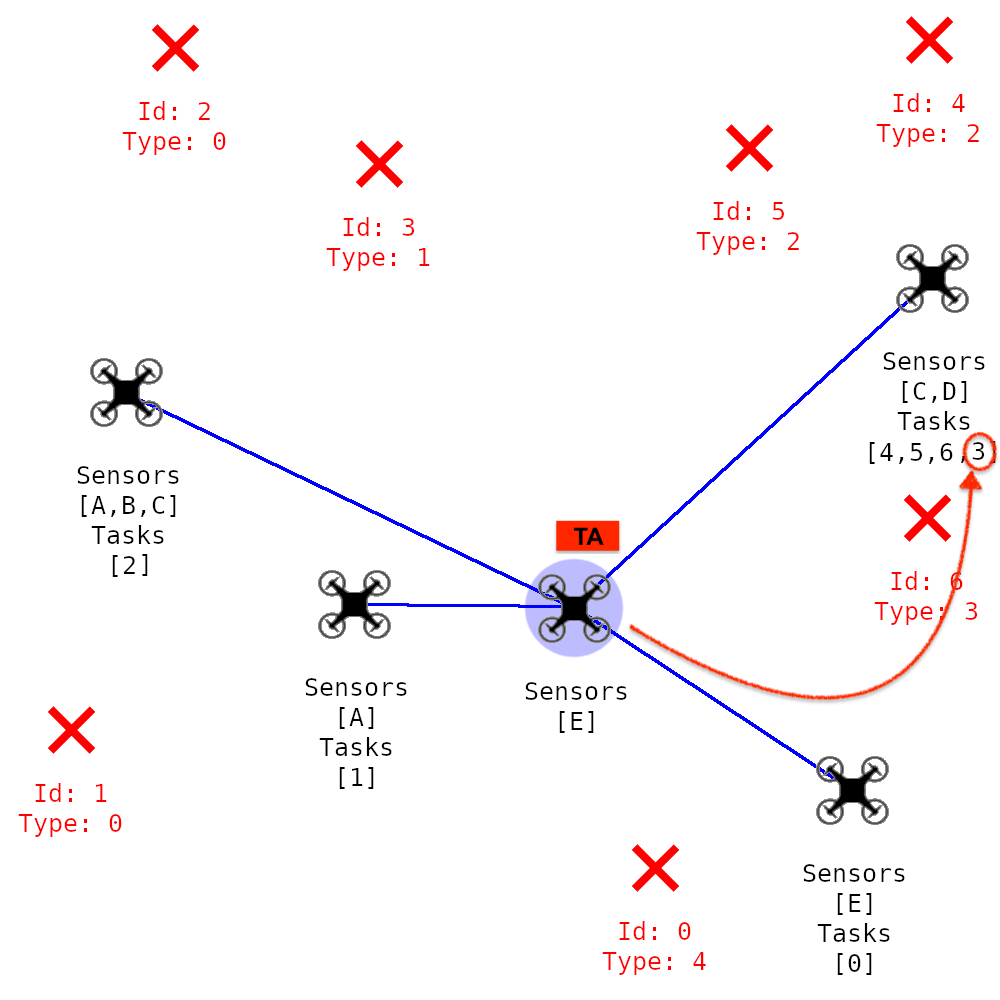
\includegraphics[width=0.95\linewidth]{img/scenario_04.png}
	    \caption{TA finds another member with a suitable sensor to send the task received \label{fig:scene04}}
	\end{subfigure}
	\caption{A task reallocation (task \#3) performed by a member with Task Allocator role, based on its compatibility's degree with the members' onboard sensors}
	\label{fig:TA_behavior}
\end{figure}


%Furthermore, the PG can absorb new tasks ($T_{add}$) added to the mission through the action $addTasks$, causing the mission update, represented by $T'++T_{add}$. 




\subsubsection{C2 Approach Manager}

At the coarsest-grained level of coordination, C2AM specifies a C2 approach change protocol, as defined formally in Figure~\ref{fig:c2a_pg}. C2AM starts operation by receiving mission tasks, member information, and initial C2 approach from the C2CS call ($g_0$ at location \textit{Notifying}), i.e., mission startup. From this initial location, it goes to the location \textit{Operating} with the initial C2 approach $\omega_0$ and sends the set of tasks $T$, the team $E$ and the $\omega_0$ over the synchronous channel $ch_2$. The C2AM remains in the $Operating$ location until eventually receiving, from TA, the pair formed by the set of unallocated tasks and the updated team members. Such information comes over the synchronous channel $ch_3$ and takes C2AM to location \textit{Maneuvering}.

The tasks received and the last information about the members' status are analyzed with the action $update$. \X{The function~\emph{find\_maneuver} takes the next C2 approach with higher awareness (cf. Section~\ref{sec:background}), according to~\citet{nato01}, and it checks if this choice is suitable for dealing with the context. In case this function finds a C2 Approach to be applied in order to perform the tasks with the available team, it is defined and the C2AM sends mission tasks, members' information and C2 Approach selected to the TA over the synchronous channel $ch_2$, then moving to the location \emph{Operating}.} Otherwise, those tasks are registered as failed ($T_{fail}$) and the TA is notified with an empty set of tasks. The C2AM then goes to location \emph{Operating} passing through \emph{Notifying} and adopts a domain defined C2 Approach $w_f$ (cf. Section~\ref{ssec:background_c2}). \X{The results of these steps is shown in Figure~\ref{fig:TeamExecutionAfterManuever}.}

\begin{figure}[!ht]
    \centering
    \scalebox{.65}{

\tikzset{every picture/.style={line width=0.75pt}} %set default line width to 0.75pt        

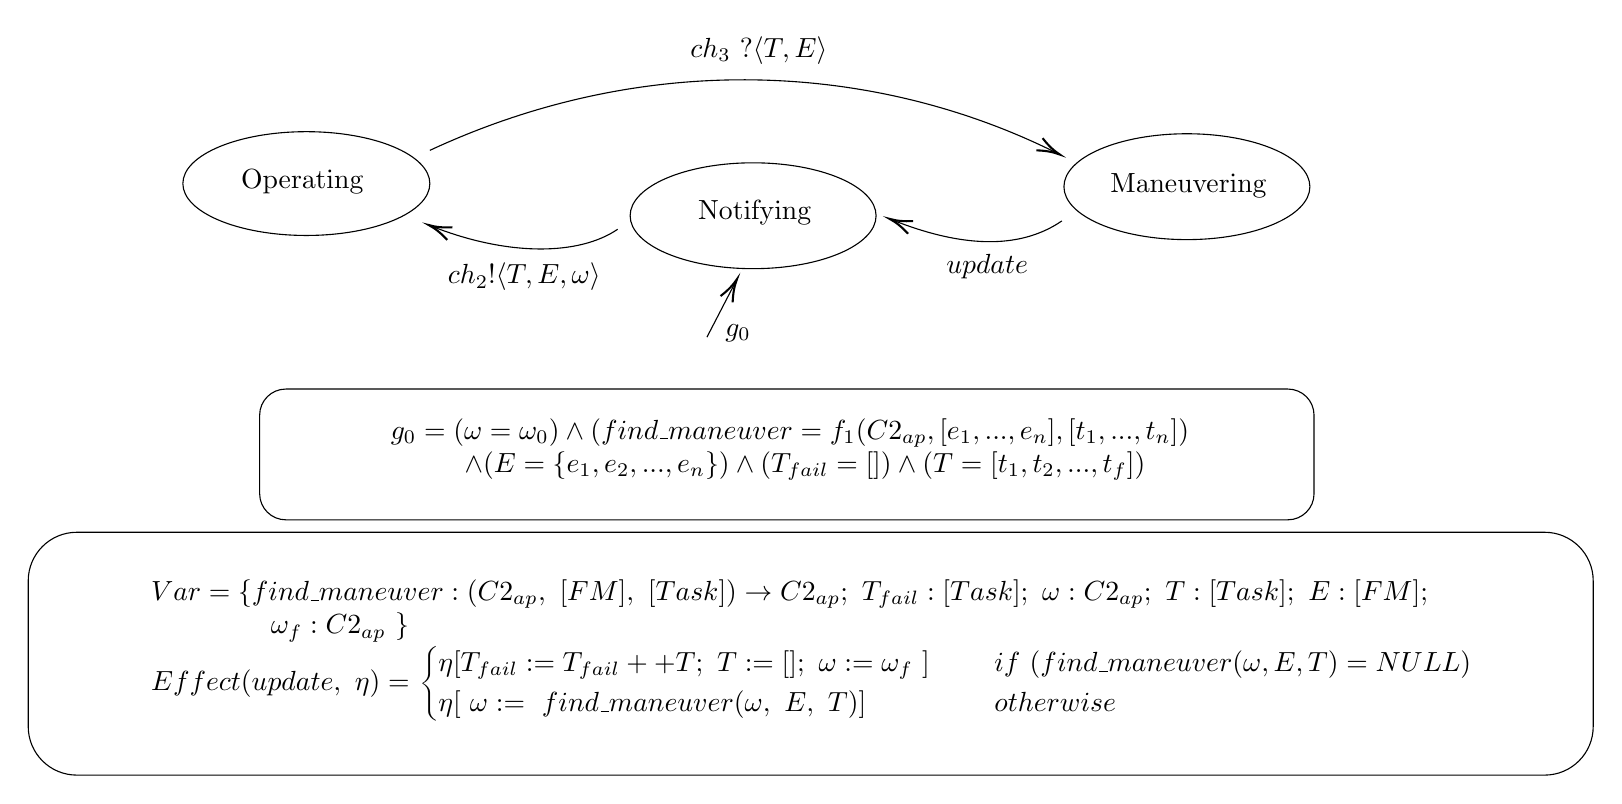
\begin{tikzpicture}[x=0.75pt,y=0.75pt,yscale=-1,xscale=1]
%uncomment if require: \path (0,370); %set diagram left start at 0, and has height of 370

%Curve Lines [id:da9480858267519683] 
\draw    (200.5,59) .. controls (307.46,9.25) and (417.89,17.91) .. (502.72,60.36) ;
\draw [shift={(504,61)}, rotate = 206.82999999999998] [color={rgb, 255:red, 0; green, 0; blue, 0 }  ][line width=0.75]    (10.93,-3.29) .. controls (6.95,-1.4) and (3.31,-0.3) .. (0,0) .. controls (3.31,0.3) and (6.95,1.4) .. (10.93,3.29)   ;
%Shape: Ellipse [id:dp6594609066072359] 
\draw   (81.5,75) .. controls (81.5,61.19) and (108.14,50) .. (141,50) .. controls (173.86,50) and (200.5,61.19) .. (200.5,75) .. controls (200.5,88.81) and (173.86,100) .. (141,100) .. controls (108.14,100) and (81.5,88.81) .. (81.5,75) -- cycle ;
%Shape: Ellipse [id:dp873836537729809] 
\draw   (506,76.5) .. controls (506,62.42) and (532.53,51) .. (565.25,51) .. controls (597.97,51) and (624.5,62.42) .. (624.5,76.5) .. controls (624.5,90.58) and (597.97,102) .. (565.25,102) .. controls (532.53,102) and (506,90.58) .. (506,76.5) -- cycle ;
%Straight Lines [id:da37650774099478246] 
\draw    (334,149) -- (347.58,122.78) ;
\draw [shift={(348.5,121)}, rotate = 477.38] [color={rgb, 255:red, 0; green, 0; blue, 0 }  ][line width=0.75]    (10.93,-3.29) .. controls (6.95,-1.4) and (3.31,-0.3) .. (0,0) .. controls (3.31,0.3) and (6.95,1.4) .. (10.93,3.29)   ;
%Rounded Rect [id:dp20897962983691354] 
\draw   (118.5,186.6) .. controls (118.5,179.64) and (124.14,174) .. (131.1,174) -- (613.9,174) .. controls (620.86,174) and (626.5,179.64) .. (626.5,186.6) -- (626.5,224.4) .. controls (626.5,231.36) and (620.86,237) .. (613.9,237) -- (131.1,237) .. controls (124.14,237) and (118.5,231.36) .. (118.5,224.4) -- cycle ;
%Rounded Rect [id:dp6489541210438411] 
\draw   (7,266.4) .. controls (7,253.48) and (17.48,243) .. (30.4,243) -- (737.6,243) .. controls (750.52,243) and (761,253.48) .. (761,266.4) -- (761,336.6) .. controls (761,349.52) and (750.52,360) .. (737.6,360) -- (30.4,360) .. controls (17.48,360) and (7,349.52) .. (7,336.6) -- cycle ;
%Shape: Ellipse [id:dp35747792046006877] 
\draw   (297,90.5) .. controls (297,76.42) and (323.53,65) .. (356.25,65) .. controls (388.97,65) and (415.5,76.42) .. (415.5,90.5) .. controls (415.5,104.58) and (388.97,116) .. (356.25,116) .. controls (323.53,116) and (297,104.58) .. (297,90.5) -- cycle ;
%Curve Lines [id:da035475864760055154] 
\draw    (424.21,92.88) .. controls (460.08,106.96) and (486.38,105.74) .. (505,93) ;
\draw [shift={(422,92)}, rotate = 22.07] [color={rgb, 255:red, 0; green, 0; blue, 0 }  ][line width=0.75]    (10.93,-3.29) .. controls (6.95,-1.4) and (3.31,-0.3) .. (0,0) .. controls (3.31,0.3) and (6.95,1.4) .. (10.93,3.29)   ;
%Curve Lines [id:da19760874620395663] 
\draw    (202.22,95.88) .. controls (238.39,109.99) and (272.38,109.74) .. (291,97) ;
\draw [shift={(200,95)}, rotate = 22.07] [color={rgb, 255:red, 0; green, 0; blue, 0 }  ][line width=0.75]    (10.93,-3.29) .. controls (6.95,-1.4) and (3.31,-0.3) .. (0,0) .. controls (3.31,0.3) and (6.95,1.4) .. (10.93,3.29)   ;

% Text Node
\draw (139,74) node   [align=left] {Operating};
% Text Node
\draw (566,76) node   [align=left] {Maneuvering};
% Text Node
\draw (359,11) node    {$ch_{3} \ ?\langle T,E\rangle $};
% Text Node
\draw (349,147) node    {$g_{0}$};
% Text Node
\draw (469,115) node    {$update$};
% Text Node
\draw (374,203) node    {$ \begin{array}{l}
g_{0} =( \omega =\omega _{0}) \land ( find\_maneuver=f_{1}( C2_{ap} ,[ e_{1} ,...,e_{n}] ,[ t_{1} ,...,t_{n}])\\
\ \ \ \ \ \ \ \ \land ( E=\{e_{1} ,e_{2} ,...,e_{n}\}) \land ( T_{fail} =[]) \land ( T=[ t_{1} ,t_{2} ,...,t_{f}])
\end{array}$};
% Text Node
\draw (385,300) node    {$ \begin{array}{l}
Var=\{find\_maneuver:( C2_{ap} ,\ [ FM] ,\ [ Task])\rightarrow C2_{ap} ;\ T_{fail} :[ Task] ;\ \omega :C2_{ap} ;\ T:[ Task] ;\ E:[ FM] ;\\
\ \ \ \ \ \ \ \ \ \ \ \ \ \omega _{f} :C2_{ap} \ \}\\
Effect( update,\ \eta ) =\begin{cases}
\eta [ T_{fail} :=T_{fail} ++T;\ T:=[] ;\ \omega :=\omega _{f} \ ] & \ \ \ \ if\ ( find\_maneuver( \omega ,E,T) =NULL)\\
\eta [ \ \omega :=\ find\_maneuver( \omega ,\ E,\ T)] & \ \ \ \ otherwise
\end{cases}
\end{array}$};
% Text Node
\draw (246,120) node    {$ch_{2} !\langle T,E,\omega \rangle $};
% Text Node
\draw (357,89) node   [align=left] {Notifying};


\end{tikzpicture}}
    \caption{Program Graph defining the C2 Approach Manager (C2AM) role}
    \label{fig:c2a_pg}
\end{figure}




%\section{Design and Implementation}
%\label{sec:designImpl}
%\input{tex/designImpl}


\section{Empirical Evaluation} 
\label{sec:evaluation}
This section presents the assessment of the model proposed in Section~\ref{sec:proposal} under different scenarios to measure the obtained C2 System agility. This assessment is performed through an \textit{in silico} experiment~\citep{simulation01} simulating UAVs dispatched on a reconnaissance mission to acquire images from a terrain. Such a method provides a way to analyze different situations and it allows us to work with different scenarios that would otherwise be unfeasible to test given incurred cost and resource availability. The simulated environment considers that the circumstances can change during the mission execution, allowing to test the effectiveness of the C2 System under such conditions. The replication package comprising the artifacts related to this empirical evaluation is available in a public repository.\footnote{\reproductibility}

The following sections present the goal definition and the metrics applied in the evaluation  (Section~\ref{ssec:definition}), the planning of the study  (Section~\ref{ssec:planning}), its execution (Section~\ref{subsec:operations}) and lastly, \X{analysis} of the obtained results and discussion about the findings  (Section~\ref{subsec:analysis_discussion}). 


 
%%%%%%%%%%%%%%%%%%%%%%%%%%%%%%%%%%
% SUBSECTION 
%%%%%%%%%%%%%%%%%%%%%%%%%%%%%%%%%%
\subsection{Definition}
\label{ssec:definition}

The performed empirical study is defined according to the Goal-Question-Metric (GQM)~\citep{gqm001} method. Figure~\ref{fig:gqm} shows the goal as the assessment of C2 Agility in our proposed computational model. The assessment made is useful to the entities' commanders. Such entities may be composed of internal entities, recursively, up to the level of individual members who also have commanders. From the goal, two research questions are derived, which consider the members within the same C2 Approach  (\textit{Q1}) and C2 Approach changes  (\textit{Q2}). Such questions address the level of C2 Agility existing in the system. Table \ref{table:metrics} defines the metrics applied in the evaluation to answer the proposed questions and corresponding agility enablers. The metrics are (\textit{M1 - Reconfigurations; M2 - Maneuvering; M3 - Engagement Time; M4 - Effectiveness; M5 - Resilience; M6 - Reward}) related to the agility enablers described by~\citet{Gren2019AgilityIR}, \citet{c2-02} and \citet{Alberts2011}.  


\begin{figure}[ht]
    \centering
    \scalebox{.52}{

\tikzset{every picture/.style={line width=0.75pt}} %set default line width to 0.75pt        

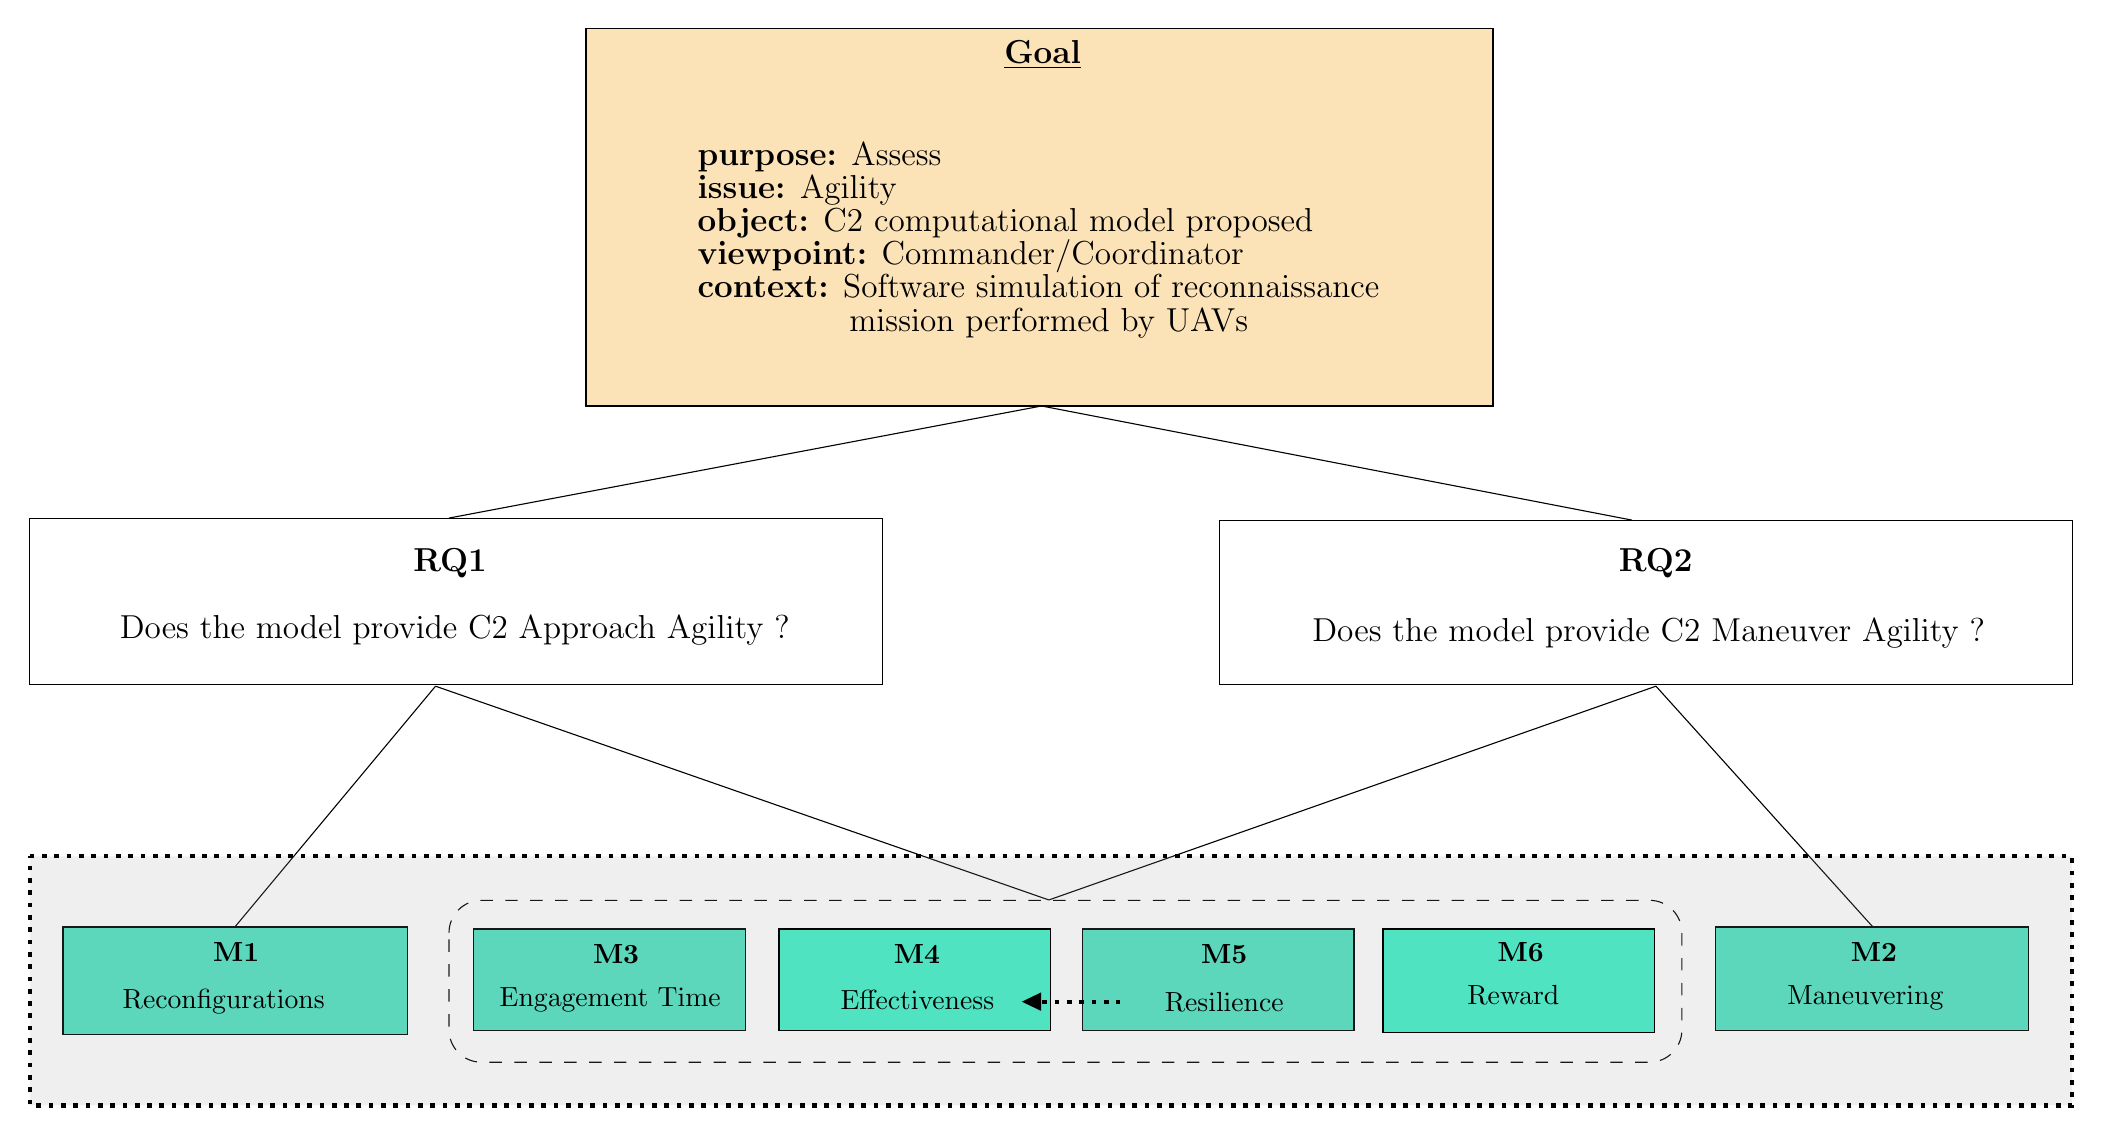
\begin{tikzpicture}[x=0.75pt,y=0.75pt,yscale=-1,xscale=1]
%uncomment if require: \path (0,532); %set diagram left start at 0, and has height of 532

%Flowchart: Process [id:dp9228173025001839] 
\draw  [fill={rgb, 255:red, 245; green, 166; blue, 35 }  ,fill opacity=0.33 ] (286.5,2) -- (723.5,2) -- (723.5,184) -- (286.5,184) -- cycle ;
%Shape: Rectangle [id:dp9468174970136011] 
\draw   (591.5,239) -- (1002.5,239) -- (1002.5,318) -- (591.5,318) -- cycle ;
%Shape: Rectangle [id:dp09665993774558346] 
\draw   (18.5,238) -- (429.5,238) -- (429.5,318) -- (18.5,318) -- cycle ;
%Straight Lines [id:da1961523796551078] 
\draw    (506,184) -- (220.5,238) ;
%Straight Lines [id:da6120336423295578] 
\draw    (506,184) -- (790.5,239) ;
%Shape: Rectangle [id:dp8704718643302001] 
\draw  [fill={rgb, 255:red, 80; green, 227; blue, 194 }  ,fill opacity=1 ] (232.5,436) -- (363.5,436) -- (363.5,485) -- (232.5,485) -- cycle ;
%Rounded Rect [id:dp2310824766673354] 
\draw  [dash pattern={on 4.5pt off 4.5pt}] (220.5,437.77) .. controls (220.5,429.15) and (227.48,422.17) .. (236.1,422.17) -- (798.9,422.17) .. controls (807.52,422.17) and (814.5,429.15) .. (814.5,437.77) -- (814.5,484.57) .. controls (814.5,493.18) and (807.52,500.17) .. (798.9,500.17) -- (236.1,500.17) .. controls (227.48,500.17) and (220.5,493.18) .. (220.5,484.57) -- cycle ;
%Straight Lines [id:da04635172987230718] 
\draw    (214,319) -- (116.5,436) ;
%Shape: Rectangle [id:dp16323070417268737] 
\draw  [fill={rgb, 255:red, 80; green, 227; blue, 194 }  ,fill opacity=1 ] (34.5,435) -- (200.5,435) -- (200.5,487) -- (34.5,487) -- cycle ;
%Straight Lines [id:da004791401702264886] 
\draw    (214,319) -- (509.5,422) ;
%Straight Lines [id:da9733307686397392] 
\draw    (802,319) -- (509.5,422) ;
%Straight Lines [id:da4492045519053316] 
\draw    (802,319) -- (906.5,435) ;
%Shape: Rectangle [id:dp7181001754521874] 
\draw  [fill={rgb, 255:red, 80; green, 227; blue, 194 }  ,fill opacity=1 ] (830.5,435) -- (981.5,435) -- (981.5,485) -- (830.5,485) -- cycle ;
%Shape: Rectangle [id:dp46797453967825375] 
\draw  [fill={rgb, 255:red, 80; green, 227; blue, 194 }  ,fill opacity=1 ] (525.5,436) -- (656.5,436) -- (656.5,485) -- (525.5,485) -- cycle ;
%Rounded Rect [id:dp9444454858651523] 
\draw  [fill={rgb, 255:red, 155; green, 155; blue, 155 }  ,fill opacity=0.16 ][dash pattern={on 1.69pt off 2.76pt}][line width=1.5]  (18.5,401) .. controls (18.5,401) and (18.5,401) .. (18.5,401) -- (1002.5,401) .. controls (1002.5,401) and (1002.5,401) .. (1002.5,401) -- (1002.5,521) .. controls (1002.5,521) and (1002.5,521) .. (1002.5,521) -- (18.5,521) .. controls (18.5,521) and (18.5,521) .. (18.5,521) -- cycle ;
%Shape: Rectangle [id:dp6205174536004793] 
\draw  [fill={rgb, 255:red, 80; green, 227; blue, 194 }  ,fill opacity=1 ] (379.5,436) -- (510.5,436) -- (510.5,485) -- (379.5,485) -- cycle ;
%Straight Lines [id:da0036921302300286785] 
\draw [line width=1.5]  [dash pattern={on 1.69pt off 2.76pt}]  (500.5,471) -- (544,471) ;
\draw [shift={(496.5,471)}, rotate = 0] [fill={rgb, 255:red, 0; green, 0; blue, 0 }  ][line width=0.08]  [draw opacity=0] (9.29,-4.46) -- (0,0) -- (9.29,4.46) -- cycle    ;
%Shape: Rectangle [id:dp36331169023965726] 
\draw  [fill={rgb, 255:red, 80; green, 227; blue, 194 }  ,fill opacity=1 ] (670.5,436) -- (801.5,436) -- (801.5,486) -- (670.5,486) -- cycle ;

% Text Node
\draw (506.5,15) node  [font=\normalsize] [align=left] {\textbf{\underline{{\large Goal}}}};
% Text Node
\draw (221,260) node   [align=left] {\textbf{{\large RQ1}}};
% Text Node
\draw (223.25,292) node   [align=left] {{\large Does the model provide C2 Approach Agility ?}};
% Text Node
\draw (798.5,293.5) node   [align=left] {{\large Does the model provide C2 Maneuver Agility ?}};
% Text Node
\draw (801.92,260) node   [align=left] {\textbf{{\large RQ2}}};
% Text Node
\draw (504.5,104) node   [align=left] {{\large \textbf{purpose:} Assess}\\{\large \textbf{issue:} Agility}\\{\large \textbf{object:} C2 computational model proposed}\\{\large \textbf{viewpoint:} Commander/Coordinator}\\{\large \textbf{context:} Software simulation of reconnaissance }\\{\large  \ \ \ \ \ \ \ \ \ \ \ \ \ \ mission performed by UAVs}};
% Text Node
\draw (301,448) node   [align=left] {\textbf{M3}};
% Text Node
\draw (118,447) node   [align=left] {\textbf{M1}};
% Text Node
\draw (907,447) node   [align=left] {\textbf{M2}};
% Text Node
\draw (298.17,470.17) node   [align=left] {Engagement Time};
% Text Node
\draw (594,448) node   [align=left] {\textbf{M5}};
% Text Node
\draw (446.17,470.17) node   [align=left] {Effectiveness};
% Text Node
\draw (446,448) node   [align=left] {\textbf{M4}};
% Text Node
\draw (594,471) node   [align=left] {Resilience};
% Text Node
\draw (62,464) node [anchor=north west][inner sep=0.75pt]   [align=left] {Reconfigurations};
% Text Node
\draw (864,462) node [anchor=north west][inner sep=0.75pt]   [align=left] {Maneuvering};
% Text Node
\draw (736.87,447) node   [align=left] {\textbf{M6}};
% Text Node
\draw (709.87,462) node [anchor=north west][inner sep=0.75pt]   [align=left] {Reward};


\end{tikzpicture}}
    \caption{GQM Diagram with the Goal, the Research Questions RQ1 and RQ2, and the metrics (M1, M2, M3, M4, M5 and M6)}
    \label{fig:gqm}
\end{figure}


\begin{table}[ht!]
	\small
	\fontsize{10}{10}\selectfont
	\centering
	\caption{Metrics used to evaluate the proposal}
	\label{table:metrics}
	
	\begin{tabularx}{\textwidth}{llXX}
	\hline
		\textbf{ID}
		& \textbf{Metric}
		& \textbf{Description} \\ [1ex]
	\hline	
	
	M1 & Reconfigurations & Number of internal reconfigurations performed by the members to accomplish the mission within a given timeout.
	\\[1ex] \\
	
	M2 & Maneuvering & Number of C2 Approach changes performed by the members to accomplish the mission within a given timeout.
	\\[1ex] \\
	
	M3 & Engagement Time & System time, in ticks, during which the entities were engaged in the execution of the tasks.
	\\[1ex] \\
	
	M4 & Effectiveness &  Percentage of successful tasks completed by the executors.
	\\[1ex] \\
	
	M5 & Resilience & System's capacity to obtain the same effectiveness of scenarios without context changes when dealing with new contexts.
	\\[1ex] \\
	
	M6 & Reward & Total quality of all sensors used to perform the tasks\\ 
	\\[1ex]
	\hline
	\end{tabularx}
\end{table} 


Context perturbations, e.g., sudden changes in the environment, or onboard component damage, require system adaptation to keep running. To identify the system's adaptation ability, the number of \color{black}member reconfigurations (M1) \color{black}and C2 Approach changes (M2) are counted. The Maneuvering (M2) metric assesses the adaptability level of the system due to its capability of \color{black} changing its organization. Response time \color{black} is measured by the Engagement Time (M3) metric, which measures how long the system takes to execute the mission's tasks. Such an aspect highlights the responsiveness of the system to changing circumstances. \X{ The Effectiveness (M4) metric evaluates the ratio of the mission’s tasks that the members have already accomplished with the total number of tasks.} 

The difference between the effectiveness (M4) metric obtained from scenarios with and without context changes shows the system capacity to recover the highest effectiveness level obtained from the scenario without context changes. Such recovery capacity defines the Resilience (M5) metric. Finally, Reward (M6) defines  the compatibility between the members and the \color{black}mission's tasks. \color{black}Equation~\ref{eq:reward} defines this metric in terms of the compatibility score $Q_{ij}$ sum.

\begin{equation}
    \label{eq:reward}
    M6=\sum Q_{ij} \ ,where\  t_j \in T_{success} \ and\ compatible(c_i,t_j)
\end{equation}

This score defines the compatibility level of a task $j$, which has a type, with a sensor $i$ used to perform it. Such a sensor corresponds to a feature in the configuration $c_i$ run by the member, and all tasks successfully performed are stored in $T_{success}$ for results analysis. Besides, all tasks with the same type have the same compatibility level to the sensors.


%%%%%%%%%%%%%%%%%%%%%%%%%%%%%%%%%%
% SUBSECTION 
%%%%%%%%%%%%%%%%%%%%%%%%%%%%%%%%%%
\subsection{Planning}
\label{ssec:planning}

The following sections describe the hypotheses on the proposed model (Section~\ref{sssec:hyp}), define the simulation scenarios  (Section~\ref{sssec:scenarios}), explain the experimental design and the analysis procedure (Section~\ref{sssec:design}), and the supporting instrumentation (Section~\ref{sssec:instrumentation}).


\subsubsection{Hypotheses Formulation}
\label{sssec:hyp}

Figure~\ref{fig:variables} shows the factors and the dependent variables related to the GQM (Figure~\ref{fig:gqm}). The scenario and the action method are identified as factors. A scenario comprises an initial context and a sequence of events that occur during the mission. Section~\ref{sssec:scenarios} details possible scenarios.

\begin{figure}[ht!]
    \centering
    \scalebox{.55}{

\tikzset{every picture/.style={line width=0.75pt}} %set default line width to 0.75pt        

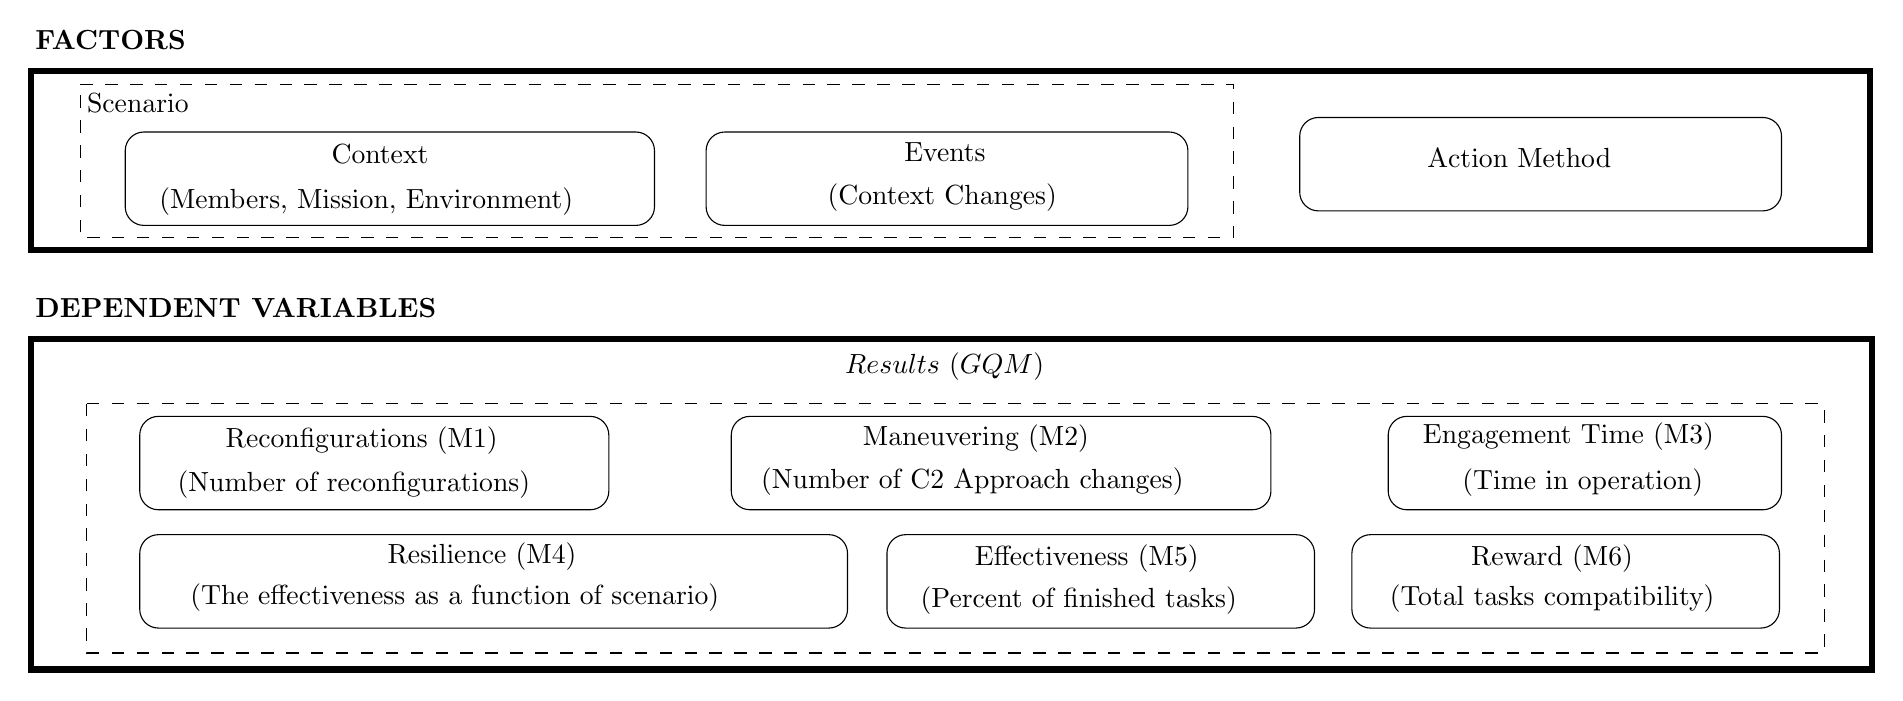
\begin{tikzpicture}[x=0.75pt,y=0.75pt,yscale=-1,xscale=1]
%uncomment if require: \path (0,322); %set diagram left start at 0, and has height of 322

%Rounded Rect [id:dp26709545620813635] 
\draw   (57.5,200) .. controls (57.5,195.03) and (61.53,191) .. (66.5,191) -- (274.5,191) .. controls (279.47,191) and (283.5,195.03) .. (283.5,200) -- (283.5,227) .. controls (283.5,231.97) and (279.47,236) .. (274.5,236) -- (66.5,236) .. controls (61.53,236) and (57.5,231.97) .. (57.5,227) -- cycle ;
%Shape: Rectangle [id:dp7868821488097882] 
\draw  [dash pattern={on 4.5pt off 4.5pt}] (32,185) -- (869,185) -- (869,305) -- (32,305) -- cycle ;
%Shape: Rectangle [id:dp07661178173797467] 
\draw  [line width=2.25]  (5,153.88) -- (892,153.88) -- (892,313) -- (5,313) -- cycle ;
%Rounded Rect [id:dp7819847156561298] 
\draw   (50.5,63) .. controls (50.5,58.03) and (54.53,54) .. (59.5,54) -- (296.5,54) .. controls (301.47,54) and (305.5,58.03) .. (305.5,63) -- (305.5,90) .. controls (305.5,94.97) and (301.47,99) .. (296.5,99) -- (59.5,99) .. controls (54.53,99) and (50.5,94.97) .. (50.5,90) -- cycle ;
%Shape: Rectangle [id:dp10398748207162001] 
\draw  [dash pattern={on 4.5pt off 4.5pt}] (28.85,31) -- (584.5,31) -- (584.5,105) -- (28.85,105) -- cycle ;
%Shape: Rectangle [id:dp48323694433186415] 
\draw  [line width=2.25]  (5,24.77) -- (891,24.77) -- (891,111) -- (5,111) -- cycle ;
%Rounded Rect [id:dp14086907660692627] 
\draw   (330.37,63) .. controls (330.37,58.03) and (334.4,54) .. (339.37,54) -- (553.5,54) .. controls (558.47,54) and (562.5,58.03) .. (562.5,63) -- (562.5,90) .. controls (562.5,94.97) and (558.47,99) .. (553.5,99) -- (339.37,99) .. controls (334.4,99) and (330.37,94.97) .. (330.37,90) -- cycle ;
%Rounded Rect [id:dp8800855997802748] 
\draw   (616.37,56) .. controls (616.37,51.03) and (620.4,47) .. (625.37,47) -- (839.5,47) .. controls (844.47,47) and (848.5,51.03) .. (848.5,56) -- (848.5,83) .. controls (848.5,87.97) and (844.47,92) .. (839.5,92) -- (625.37,92) .. controls (620.4,92) and (616.37,87.97) .. (616.37,83) -- cycle ;
%Rounded Rect [id:dp41591552385229413] 
\draw   (659,200) .. controls (659,195.03) and (663.03,191) .. (668,191) -- (839.5,191) .. controls (844.47,191) and (848.5,195.03) .. (848.5,200) -- (848.5,227) .. controls (848.5,231.97) and (844.47,236) .. (839.5,236) -- (668,236) .. controls (663.03,236) and (659,231.97) .. (659,227) -- cycle ;
%Rounded Rect [id:dp6557542326475674] 
\draw   (342.5,200) .. controls (342.5,195.03) and (346.53,191) .. (351.5,191) -- (593.5,191) .. controls (598.47,191) and (602.5,195.03) .. (602.5,200) -- (602.5,227) .. controls (602.5,231.97) and (598.47,236) .. (593.5,236) -- (351.5,236) .. controls (346.53,236) and (342.5,231.97) .. (342.5,227) -- cycle ;
%Rounded Rect [id:dp018207773722970888] 
\draw   (641.5,257) .. controls (641.5,252.03) and (645.53,248) .. (650.5,248) -- (838.5,248) .. controls (843.47,248) and (847.5,252.03) .. (847.5,257) -- (847.5,284) .. controls (847.5,288.97) and (843.47,293) .. (838.5,293) -- (650.5,293) .. controls (645.53,293) and (641.5,288.97) .. (641.5,284) -- cycle ;
%Rounded Rect [id:dp7136990985847002] 
\draw   (57.5,257) .. controls (57.5,252.03) and (61.53,248) .. (66.5,248) -- (389.5,248) .. controls (394.47,248) and (398.5,252.03) .. (398.5,257) -- (398.5,284) .. controls (398.5,288.97) and (394.47,293) .. (389.5,293) -- (66.5,293) .. controls (61.53,293) and (57.5,288.97) .. (57.5,284) -- cycle ;
%Rounded Rect [id:dp3168441468736909] 
\draw   (417.5,257) .. controls (417.5,252.03) and (421.53,248) .. (426.5,248) -- (614.5,248) .. controls (619.47,248) and (623.5,252.03) .. (623.5,257) -- (623.5,284) .. controls (623.5,288.97) and (619.47,293) .. (614.5,293) -- (426.5,293) .. controls (421.53,293) and (417.5,288.97) .. (417.5,284) -- cycle ;

% Text Node
\draw (396.1,159.07) node [anchor=north west][inner sep=0.75pt]    {$Results\ ( GQM)$};
% Text Node
\draw (6,133) node [anchor=north west][inner sep=0.75pt]   [align=left] {\textbf{DEPENDENT VARIABLES}};
% Text Node
\draw (148.64,58.62) node [anchor=north west][inner sep=0.75pt]   [align=left] {Context};
% Text Node
\draw (6,4) node [anchor=north west][inner sep=0.75pt]   [align=left] {\textbf{FACTORS}};
% Text Node
\draw (65.64,79.62) node [anchor=north west][inner sep=0.75pt]   [align=left] {(Members, Mission, Environment)};
% Text Node
\draw (424.64,57.62) node [anchor=north west][inner sep=0.75pt]   [align=left] {Events};
% Text Node
\draw (387.64,77.62) node [anchor=north west][inner sep=0.75pt]   [align=left] {(Context Changes)};
% Text Node
\draw (676.64,60.62) node [anchor=north west][inner sep=0.75pt]   [align=left] {Action Method};
% Text Node
\draw (693.5,215) node [anchor=north west][inner sep=0.75pt]   [align=left] {(Time in operation)};
% Text Node
\draw (674.5,193) node [anchor=north west][inner sep=0.75pt]   [align=left] {Engagement Time (M3)};
% Text Node
\draw (30.85,34) node [anchor=north west][inner sep=0.75pt]   [align=left] {Scenario};
% Text Node
\draw (74.5,216) node [anchor=north west][inner sep=0.75pt]   [align=left] {(Number of reconfigurations)};
% Text Node
\draw (97.64,194.62) node [anchor=north west][inner sep=0.75pt]   [align=left] {Reconfigurations (M1)};
% Text Node
\draw (355.64,214.62) node [anchor=north west][inner sep=0.75pt]   [align=left] {(Number of C2 Approach changes)};
% Text Node
\draw (404.64,193.62) node [anchor=north west][inner sep=0.75pt]   [align=left] {Maneuvering (M2)};
% Text Node
\draw (658.5,271) node [anchor=north west][inner sep=0.75pt]   [align=left] {(Total tasks compatibility)};
% Text Node
\draw (697.64,251.62) node [anchor=north west][inner sep=0.75pt]   [align=left] {Reward (M6)};
% Text Node
\draw (80.64,270.62) node [anchor=north west][inner sep=0.75pt]   [align=left] {(The effectiveness as a function of scenario)};
% Text Node
\draw (175.64,250.62) node [anchor=north west][inner sep=0.75pt]   [align=left] {Resilience (M4)};
% Text Node
\draw (432.5,272) node [anchor=north west][inner sep=0.75pt]   [align=left] {(Percent of finished tasks)};
% Text Node
\draw (458.64,251.62) node [anchor=north west][inner sep=0.75pt]   [align=left] {Effectiveness (M5)};


\end{tikzpicture}}
    \caption{Factors and dependent variables used by the proposed model}
    \label{fig:variables}
\end{figure}

The second factor is called the action method and it represents the system's response to deal with a context change or perturbation. Consider two possible treatments, namely A1 and A2, which identify the baseline and the proposed model to respond to context changes, respectively. With treatment A1, the system starts the execution with an initial context, performs a task allocation of mission tasks among team members, and in face of context changes, the system just keeps running as long as it can, but it does not perform any kind of adaptation to deal with new circumstances. Such a treatment represents the low maturity of the state-of-the-art in C2 agility to deal with context changes. Indeed, especially in the military domain, e.g., ~\citet{CC03, FRANCE2014}, the proposed solutions perform only a historical analysis of success or an aleatory strategy choosing to deal with the new circumstances based on a fast and simplified analysis of some scenario variables. Another common strategy is 
not to perform any kind of adaptation to deal with new circumstances, which characterizes our baseline treatment A1. In contrast, treatment A2 applies the C2 computational model proposed in Section~\ref{sec:proposal}. 

Also, in all considered scenarios of both treatments, each task can be executed by at least one team member. It is relevant because of the baseline, where there are no \X{member reconfigurations}.
%Both treatments have all sensors type at least once. It is relevant because of the baseline, where there are no members’ reconfiguration. Such a scenario guarantees the existence of at least a member able to perform the tasks of each type. 
Considering the research questions and the metrics identified in GQM, the corresponding null and alternative hypotheses are formulated, as shown in Table \ref{table:hyp}. 

\begin{table}[ht!]
	\small
	\fontsize{11}{11}\selectfont
	\centering
	\caption{\color{black}Experimental hypotheses, where $\overline{m}$ is the average of each metric $m$ in $Metric=\{M_1, M_2, M_3, M_4, M_5, M_6\}$ and $Scenario$ is the set of scenarios composed by context and events (see Figure~\ref{fig:variables})\color{black}} 
	\label{table:hyp}
	\begin{center}
	\begin{tabularx}{0.95\textwidth}{X p{0.70\linewidth}}
	\hline
		
		\textbf{Hypothesis}
		& \textbf{Definition} \\ [1ex]
	\hline	
	
	\\ $H_0$ & $\forall m \in Metric, \forall s \in Scenario \cdot (\overline{m}(s \times A1)=\overline{m}(s \times A2)$) 
	\\[1ex] \\
	
	\\ $H_1$ & $\forall m \in Metric, \forall s \in Scenario \cdot (\overline{m}(s \times A1) \neq \overline{m}(s \times A2)$) 
	\\[1ex] \\
	
	\hline
	\end{tabularx}
	\end{center}
\end{table} 

The null hypothesis states there will be no statistically significant differences in metrics' average for different action methods in the same scenario. The alternative hypothesis states otherwise. % In $H_1$, for all metrics in GQM (Figure~\ref{fig:gqm}), i.e., M1, M2, M3, M4, M5, and M6, different results for two different treatments are collected, i.e., A1 and A2, applied to the factor agility method. This difference in results can confirm the presence of C2 agility and its impact on the system.


%%%%%%%%%%%%%%%%%%%%%%%%%%%%%%%%%%
% SUBSECTION 
%%%%%%%%%%%%%%%%%%%%%%%%%%%%%%%%%%
\subsubsection{Simulation Scenarios}
\label{sssec:scenarios}

A simulation scenario consists of an initial context and a sequence of events that provide dynamism (cf. Figure~\ref{fig:scenario}). \color{black}A regular expression was used to write the sequence of events representing the possibility of multiple occurrences of each event $\alpha_i$, which can be none or several, making up the sequence of context changes. \color{black}The initial context comprises the set $E$ of members operating an initial C2 Approach $\omega$, the mission $M$ composed of a set of tasks, and the environment. Each event in the set $CtxAct$ (see Equation~\ref{eq:ctxact})\color{black}, so-called Context Actions, \color{black}represents an action that causes a member or environment changes at runtime, i.e., changes in the context. 

\begin{equation}
    \label{eq:ctxact}
    CtxAct = \{memberFailure,sensorFailure, envChange \} 
\end{equation}

The environment represents all the conditions of the place where the members act, e.g., weather conditions, hazard due to enemy's activity, and communication restrictions. They are modeled as the state of a specific kind of onboard sensor, i.e., a foggy day can turn a VGA sensor useless.

\begin{figure}[ht!]
    \centering
    \scalebox{.5}{

\tikzset{every picture/.style={line width=0.75pt}} %set default line width to 0.75pt        

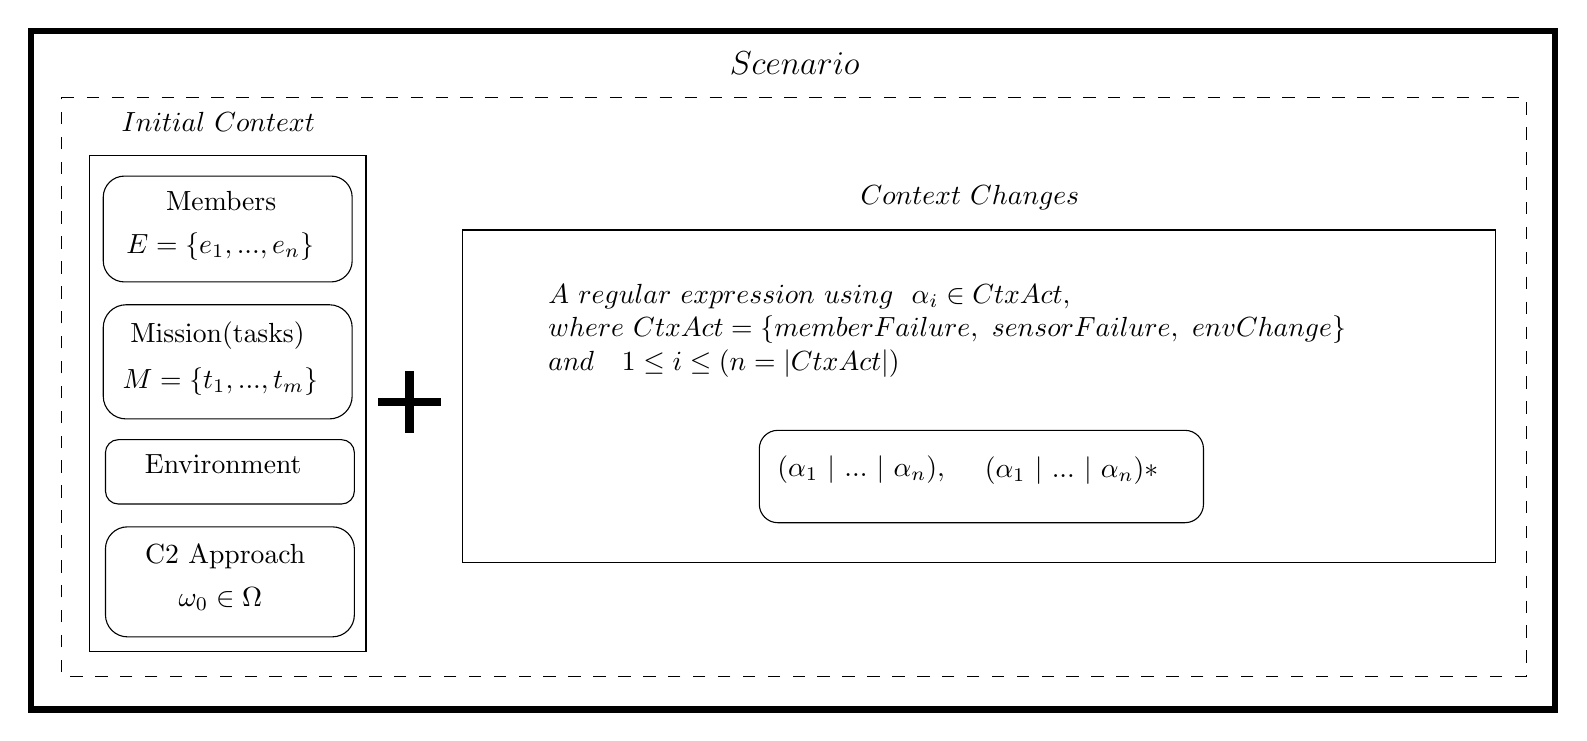
\begin{tikzpicture}[x=0.75pt,y=0.75pt,yscale=-1,xscale=1]
%uncomment if require: \path (0,349); %set diagram left start at 0, and has height of 349

%Rounded Rect [id:dp4190516071959901] 
\draw   (45.48,212.2) .. controls (45.48,208.78) and (48.25,206) .. (51.68,206) -- (159.2,206) .. controls (162.63,206) and (165.4,208.78) .. (165.4,212.2) -- (165.4,230.8) .. controls (165.4,234.22) and (162.63,237) .. (159.2,237) -- (51.68,237) .. controls (48.25,237) and (45.48,234.22) .. (45.48,230.8) -- cycle ;
%Rounded Rect [id:dp916271795400267] 
\draw   (44.41,152) .. controls (44.41,145.92) and (49.34,141) .. (55.41,141) -- (153.34,141) .. controls (159.41,141) and (164.34,145.92) .. (164.34,152) -- (164.34,185) .. controls (164.34,191.08) and (159.41,196) .. (153.34,196) -- (55.41,196) .. controls (49.34,196) and (44.41,191.08) .. (44.41,185) -- cycle ;
%Rounded Rect [id:dp6771464113681669] 
\draw   (44.41,89.2) .. controls (44.41,83.57) and (48.98,79) .. (54.61,79) -- (154.14,79) .. controls (159.77,79) and (164.34,83.57) .. (164.34,89.2) -- (164.34,119.8) .. controls (164.34,125.43) and (159.77,130) .. (154.14,130) -- (54.61,130) .. controls (48.98,130) and (44.41,125.43) .. (44.41,119.8) -- cycle ;
%Shape: Rectangle [id:dp977819802873701] 
\draw   (37.75,69) -- (171,69) -- (171,308) -- (37.75,308) -- cycle ;
%Rounded Rect [id:dp11904903891609209] 
\draw   (45.48,258.6) .. controls (45.48,252.75) and (50.22,248) .. (56.08,248) -- (154.8,248) .. controls (160.66,248) and (165.4,252.75) .. (165.4,258.6) -- (165.4,290.4) .. controls (165.4,296.25) and (160.66,301) .. (154.8,301) -- (56.08,301) .. controls (50.22,301) and (45.48,296.25) .. (45.48,290.4) -- cycle ;

%Shape: Rectangle [id:dp6932811140385843] 
\draw  [dash pattern={on 4.5pt off 4.5pt}] (24.5,41) -- (730,41) -- (730,320) -- (24.5,320) -- cycle ;
%Shape: Rectangle [id:dp3952140034216508] 
\draw  [line width=2.25]  (9.5,9) -- (744,9) -- (744,336) -- (9.5,336) -- cycle ;
%Shape: Rectangle [id:dp32385330595430617] 
\draw   (217.5,105) -- (715,105) -- (715,265) -- (217.5,265) -- cycle ;
%Rounded Rect [id:dp9646271465434701] 
\draw   (360.5,210.4) .. controls (360.5,205.48) and (364.48,201.5) .. (369.4,201.5) -- (565.6,201.5) .. controls (570.52,201.5) and (574.5,205.48) .. (574.5,210.4) -- (574.5,237.1) .. controls (574.5,242.02) and (570.52,246) .. (565.6,246) -- (369.4,246) .. controls (364.48,246) and (360.5,242.02) .. (360.5,237.1) -- cycle ;

\draw  [line width=3]  (177,188) -- (207,188)(192,173) -- (192,203) ;

% Text Node
\draw (345,18) node [anchor=north west][inner sep=0.75pt]  [font=\large]  {$Scenario$};
% Text Node
\draw (393,287) node [anchor=north west][inner sep=0.75pt]    {$\ \ $};
% Text Node
\draw (408,82) node [anchor=north west][inner sep=0.75pt]    {$Context\ Changes$};
% Text Node
\draw (52,47) node [anchor=north west][inner sep=0.75pt]    {$Initial\ Context$};
% Text Node
\draw (251,128) node [anchor=north west][inner sep=0.75pt]    {$ \begin{array}{l}
A\ regular\ expression\ using\ \ \alpha _{i} \in CtxAct,\ \\
where\ CtxAct=\{memberFailure,\ sensorFailure,\ envChange\} \ \\
and\ \ \ 1\leq i\leq ( n=|CtxAct|)
\end{array}$};
% Text Node
\draw (73.42,85) node [anchor=north west][inner sep=0.75pt]   [align=left] {Members};
% Text Node
\draw (56.17,148) node [anchor=north west][inner sep=0.75pt]   [align=left] {Mission(tasks)};
% Text Node
\draw (63.24,212) node [anchor=north west][inner sep=0.75pt]   [align=left] {Environment};
% Text Node
\draw (54.32,105) node [anchor=north west][inner sep=0.75pt]    {$E=\{e_{1} ,...,e_{n}\}$};
% Text Node
\draw (52.42,170) node [anchor=north west][inner sep=0.75pt]    {$M=\{t_{1} ,...,t_{m}\}$};
% Text Node
\draw (63.37,255) node [anchor=north west][inner sep=0.75pt]   [align=left] {C2 Approach};
% Text Node
\draw (79.49,276) node [anchor=north west][inner sep=0.75pt]    {$\omega _{0} \in \Omega $};
% Text Node
\draw (463.41,213) node [anchor=north west][inner sep=0.75pt]    {$\ ( \alpha _{1} \ |\ ...\ |\ \alpha _{n}) *$};
% Text Node
\draw (363.5,212.4) node [anchor=north west][inner sep=0.75pt]    {$\ ( \alpha _{1} \ |\ ...\ |\ \alpha _{n}) ,$};


\end{tikzpicture}}
    \caption{Scenario comprising the initial context variables and a sequence of events that characterizes a dynamic context}
    \label{fig:scenario}
\end{figure}

\X{As shown in Section~\ref{sec:example}, a dynamic context represents all the possibilities of changes: i) in the members, through unavailability of any nature; ii) in the mission, with changes in the tasks to be performed, or iii) in the environment, with disturbances in any element of the environment where the members act. However, for evaluating the system’s response to changes in the context, we selected a set of significant events that cause device damage or degradation of any nature, or any feature of status interest, depending on the specific type of system under concern. Table~\ref{table:context_changes} lists the actions related to a sample of context changes, combined with the initial context used by the simulation. These actions occur during the simulation to create a dynamic scenario, resembling realistic settings. Onboard sensors perceive environmental changes in all members and reduce their capability to be employed in a mission.}

%Table~\ref{table:context_changes} lists the possible actions combined with the initial context used by the simulation. These actions occur during the simulation to create a dynamic scenario, resembling realistic settings. Environmental changes are perceived by onboard sensors in all members and cause a reduction of their capability to be employed in a mission.


\begin{table}[ht]
	\small
	\fontsize{10}{10}\selectfont
	\centering
	\caption{Context changes handled by the simulator with related actions in the CS and their impact level in the system}
	\label{table:context_changes}

	\begin{tabular}{p{0.16\linewidth}p{0.18\linewidth}p{0.1\linewidth}p{0.43\linewidth}}
	\hline
		 \textbf{Change}
		& \textbf{Action}
		& \textbf{Impact}
		& \textbf{Description}  \\ [1ex]
	\hline	\\ [-1ex] 
	Environment & \textit{envChange} & low & Weather conditions (e.g., luminosity, cloudiness) impacting the sensor's quality; \\[1ex]
	& & & Hazard level requiring changes in the UAV's behavior \\[5ex]
	Self & \textit{sensorFailure} & medium & Sensor onboard damage caused by any internal issue (\color{blue}e.g.\color{black}, electronic circuit damaged) \\[1ex]
	& \textit{memberFailure} & high & UAV out of operation due to serious damage (e.g., no fuel or battery, or taken down) \\[6ex]
	
	%Mission & addTasks & 1 & tasks addition or removal in the mission \\[5ex]
	\hline
	\end{tabular}
\end{table} 



With military domain experts' collaboration, we classify these context change events according to their impact on the system. Such classification is based on consolidated doctrines of a situation analysis and planning in military operations with application in many different contexts~\citep{nato01, doctrine01, Fernandes2016, UAV_Aplication, CC03, UAV01}. It is used to create the sequences of events \color{black} in an increasing level of complexity\color{black}, requiring more resilience from the system. 

Table~\ref{tab:scenarios} shows the scenarios considered in the simulation. 
\color{black} The related event sequences were selected to have increasing level of complexity and commonality, based on the impact classification presented in Table~\ref{table:context_changes}, obtained from military domain experts. Accordingly, environment changes are more common to occur in the operation, followed by sensor issues and member failures because of enemy engagement or mechanical problems.
\color{black}

Besides the sequences of events presented, the initial contexts for all scenarios are formed by a team $E$ with 5 members, a mission $M$ with 30 tasks, and De-Conflicted as the initial C2 Approach $w_0$, i.e., a ring communication structure. During the simulation, these events occur in the sequence presented but at random times within the mission timeout.



\begin{table}[ht]
\centering
\fontsize{9}{9}
\selectfont
\caption{List of events (\textit{EC-envChange; SF-sensorFailure; MF-memberFailure}) that characterizes the context changes within the scenarios tested. The initial C2 Approach, the set of members $E$ and the mission $M$ remain unchanged.}
\label{tab:scenarios}
\begin{tabular}{|m{0.1\textwidth}|m{0.82\textwidth}|}
\hline
\rowcolor{lightgray}
 \textbf {Scenario} & \hfil  \textbf {Context Changes} \\
\hline  & \\[-1.5ex]
\hfil 1 & EC, EC, EC, EC, EC \\[1ex]
\hline  & \\[-1.5ex]
\hfil 2 & EC, EC, EC, EC, EC, EC, EC, EC, EC, EC, EC, EC, EC, EC, EC \\[1ex]
\hline & \\[-1.5ex]
\hfil 3 & 
EC, EC, EC, EC, EC, MF, EC, EC, EC, EC, EC, MF, EC, EC, EC, EC, EC, MF, EC, EC, EC, EC, EC  \\[1ex]
\hline & \\[-1.5ex]
\hfil 4 & EC, EC, EC, EC, EC, SF, EC, EC, EC, EC, EC, SF, EC, EC, EC, EC, EC, SF, EC, EC, EC, EC, EC  \\[1ex]
\hline & \\[-1.5ex]
 \hfil 5 & EC, EC, EC, SF, EC, EC, EC, MF, EC, EC, EC, SF, EC, EC, EC, MF, EC, EC, EC, SF, EC, EC, EC, MF  \\[1ex]
\hline & \\[-1.5ex]
 \hfil 6 & EC, SF, MF, EC, SF, EC, SF, EC, SF, MF, EC, SF, EC, SF, EC, SF \\[1ex]
\hline & \\[-1.5ex]
 \hfil 7 & MF, SF, EC, EC, EC, EC, EC, EC, EC, EC, EC, EC, MF, SF, EC, EC, EC, EC, EC, MF, SF, EC, EC, EC, MF, SF, EC \\[1ex]
 \hline & \\[-1.5ex]
 \hfil 8 & MF, SF, EC, MF, SF, EC, MF, SF, EC, MF, SF, EC \\[1.5ex]
 \hline & \\[-1.5ex] 
 \hfil 9 & SF, SF, SF, MF, SF, SF, SF, MF, SF, SF, SF, MF, SF, SF, SF \\[1ex]
 \hline & \\[-1.5ex] 
 \hfil 10 & SF, EC, MF, SF, EC, MF, SF, EC, MF, SF, EC, MF, EC, EC, EC, EC, EC, EC, EC, EC, EC, EC \\[1ex]
 \hline
\end{tabular}

\end{table}


The simulation operates a scenario with 5 possible types of tasks (0 to 4) and 5 types of sensors (A, B, C, D, and E). The tasks and onboard sensors are randomly chosen \color{black}before the round executes\color{black}. When the \color{black} task allocation \color{black}process starts, the algorithm applies a function that returns the quality $Q_{ij}$, obtained from a table, that correlates a sensor $i$ to the task $j$. When $Q_{ij}=0$ it means the sensor $i$ is not able to perform the task $j$.



%%%%%%%%%%%%%%%%%%%%%%%%%%%%%%%%%%
% SUBSECTION 
%%%%%%%%%%%%%%%%%%%%%%%%%%%%%%%%%%
\subsubsection{Experimental Design and Analysis Procedure}
\label{sssec:design}


Figure \ref{fig:exp_design} illustrates the factorial experimental design applied to assess the formulated hypotheses, where each action method is exercised with each scenario in a trial (cf. Section~\ref{sssec:scenarios}). Combinations of the factors are assessed with the metrics shown in Figure~\ref{fig:gqm}.


\begin{figure}[ht]
    \centering
    \scalebox{.6}{

\tikzset{every picture/.style={line width=0.75pt}} %set default line width to 0.75pt        

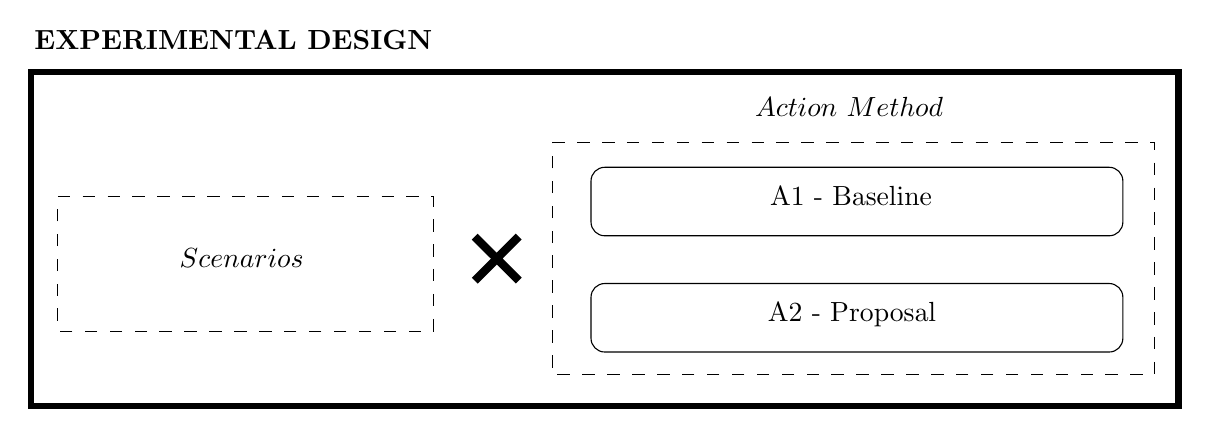
\begin{tikzpicture}[x=0.75pt,y=0.75pt,yscale=-1,xscale=1]
%uncomment if require: \path (0,201); %set diagram left start at 0, and has height of 201

%Rounded Rect [id:dp06575569211056953] 
\draw   (279.42,79.6) .. controls (279.42,75.95) and (282.37,73) .. (286.02,73) -- (529.06,73) .. controls (532.7,73) and (535.66,75.95) .. (535.66,79.6) -- (535.66,99.4) .. controls (535.66,103.05) and (532.7,106) .. (529.06,106) -- (286.02,106) .. controls (282.37,106) and (279.42,103.05) .. (279.42,99.4) -- cycle ;
%Shape: Rectangle [id:dp6932811140385843] 
\draw  [dash pattern={on 4.5pt off 4.5pt}] (22.5,87) -- (203.5,87) -- (203.5,152) -- (22.5,152) -- cycle ;
%Shape: Rectangle [id:dp9822494345299366] 
\draw  [dash pattern={on 4.5pt off 4.5pt}] (260.75,61) -- (551,61) -- (551,173) -- (260.75,173) -- cycle ;
%Shape: Rectangle [id:dp3952140034216508] 
\draw  [line width=2.25]  (9.5,27) -- (562.5,27) -- (562.5,188) -- (9.5,188) -- cycle ;
\draw  [line width=3]  (223.37,106.42) -- (244.63,127.58)(244.58,106.37) -- (223.42,127.63) ;
%Rounded Rect [id:dp9781270849297624] 
\draw   (279.42,135.6) .. controls (279.42,131.95) and (282.37,129) .. (286.02,129) -- (529.06,129) .. controls (532.7,129) and (535.66,131.95) .. (535.66,135.6) -- (535.66,155.4) .. controls (535.66,159.05) and (532.7,162) .. (529.06,162) -- (286.02,162) .. controls (282.37,162) and (279.42,159.05) .. (279.42,155.4) -- cycle ;

% Text Node
\draw (80,111) node [anchor=north west][inner sep=0.75pt]    {$Scenarios$};
% Text Node
\draw (357.17,38) node [anchor=north west][inner sep=0.75pt]    {$Action\ Method$};
% Text Node
\draw (10,6) node [anchor=north west][inner sep=0.75pt]   [align=left] {\textbf{EXPERIMENTAL DESIGN}};
% Text Node
\draw (364.41,81) node [anchor=north west][inner sep=0.75pt]   [align=left] {A1 - Baseline};
% Text Node
\draw (363.41,137) node [anchor=north west][inner sep=0.75pt]   [align=left] {A2 - Proposal};


\end{tikzpicture}}
    \caption{Factorial experimental design, where each action method is exercised with each scenario.}
    \label{fig:exp_design}
\end{figure}


The simulation uses a set of random variables to define some elements during execution, such as UAVs’ and tasks’ positions, and sensors that the context event will affect. \X{A simulator} engine generates these random numbers based on seeds created in runtime. For a consistent comparison between the action methods A1 and A2, a fixed set of seeds within the same trial were used in order to have the same value of such variables \X{during each} experimentation round.

To proceed with data analysis and sample size definition, a confidence level of 95\% in all statistical calculations was used. Such confidence level brings a significant population mean estimation and an acceptable sampling error. A \emph{p-value} of 0.05 was used to perform statistical hypothesis testing. The choice of these parameters is based on the standard cutoff used in \color{black}previous works; e.g.,~\citet{CochranW.G.1983} and~\citet{Bruce2014}. \color{black}


%%%%%%%%%%%%%%%%%%%%%%%%%%%%%%%%%%
% SUBSECTION 
%%%%%%%%%%%%%%%%%%%%%%%%%%%%%%%%%%
\subsubsection{Instrumentation}
\label{sssec:instrumentation}

Following related research on C2 simulation~\citep{FRANCE2014, Fernandes2016, Stanton2007, c2-02} and on the use of roles as components of agents' implementation~\citep{agent0010, agent1}, the simulations were performed using an agent-based framework, in this case Repast Simphony~\citep{North2013, SIMUL01, ClaesWohlinPerRuneson2012}. Figure~\ref{fig:repast01} shows an execution screen of the implementation \color{black} with the parameter fields \color{black} that can be changed to create different experimental setups \color{black} and the panel \color{black} with the agents' execution field.

The simulation implements the three roles modelled by the PGs shown in Figures \color{black} \ref{fig:ex_pg}, \ref{fig:ta_pg}, and \ref{fig:c2a_pg}  \color{black} to define UAV behavior with autonomy of reconfiguration, tasks allocation and execution, employed in a military recognition mission~\citep{UAV_Aplication}. Furthermore, perturbations and factors modifications were inserted in runtime to provide dynamism to the system and make it closer to a real scenario. A context change simulated by the system causes the quality reduction of a specific type of sensor, e.g., an environment change simulating a luminosity decreasing \color{black} reduces by $50\%$ \color{black} the quality of the sensor type 2 that represents a VGA camera. Sensor failure is modelled by setting its quality to zero. Furthermore, a member \color{black} can be lost with, consequently, \color{black} all its onboard sensors.

Inspired by the solution applied in~\citet{MAS07} and \citet{UAV01} to allocate tasks to a set of agents, a similar principle was used in this work based on swarm strategy. Depending on the C2 Approach \color{black}operating\color{black}, the members are notified about the allocation performed and unfinished tasks. This guarantees a better awareness level among entities and can improve the allocation result due to more context information shared by the members. Such allocation is feasible when a member has a configuration that activates a \color{black}task-compatible sensor\color{black}.

The C2 Approach \color{black}Maneuvering \color{black}follows the enumerated type described in Section~\ref{ssec:background_c2}. From the initial C2 Approach, which is De-Conflicted (cf. Section~\ref{sssec:scenarios}), the maneuver follows incrementally over this list and going back to Conflicted after Edge. The Conflicted is the final C2 Approach adopted by the system before discarding the unfeasible tasks. Such sequence is based on real scenarios of the military domain where a disconnected structure is adopted in extreme situations where there are no conditions to hold another communication and interaction strategy.


\begin{figure}[ht]
  \centering
  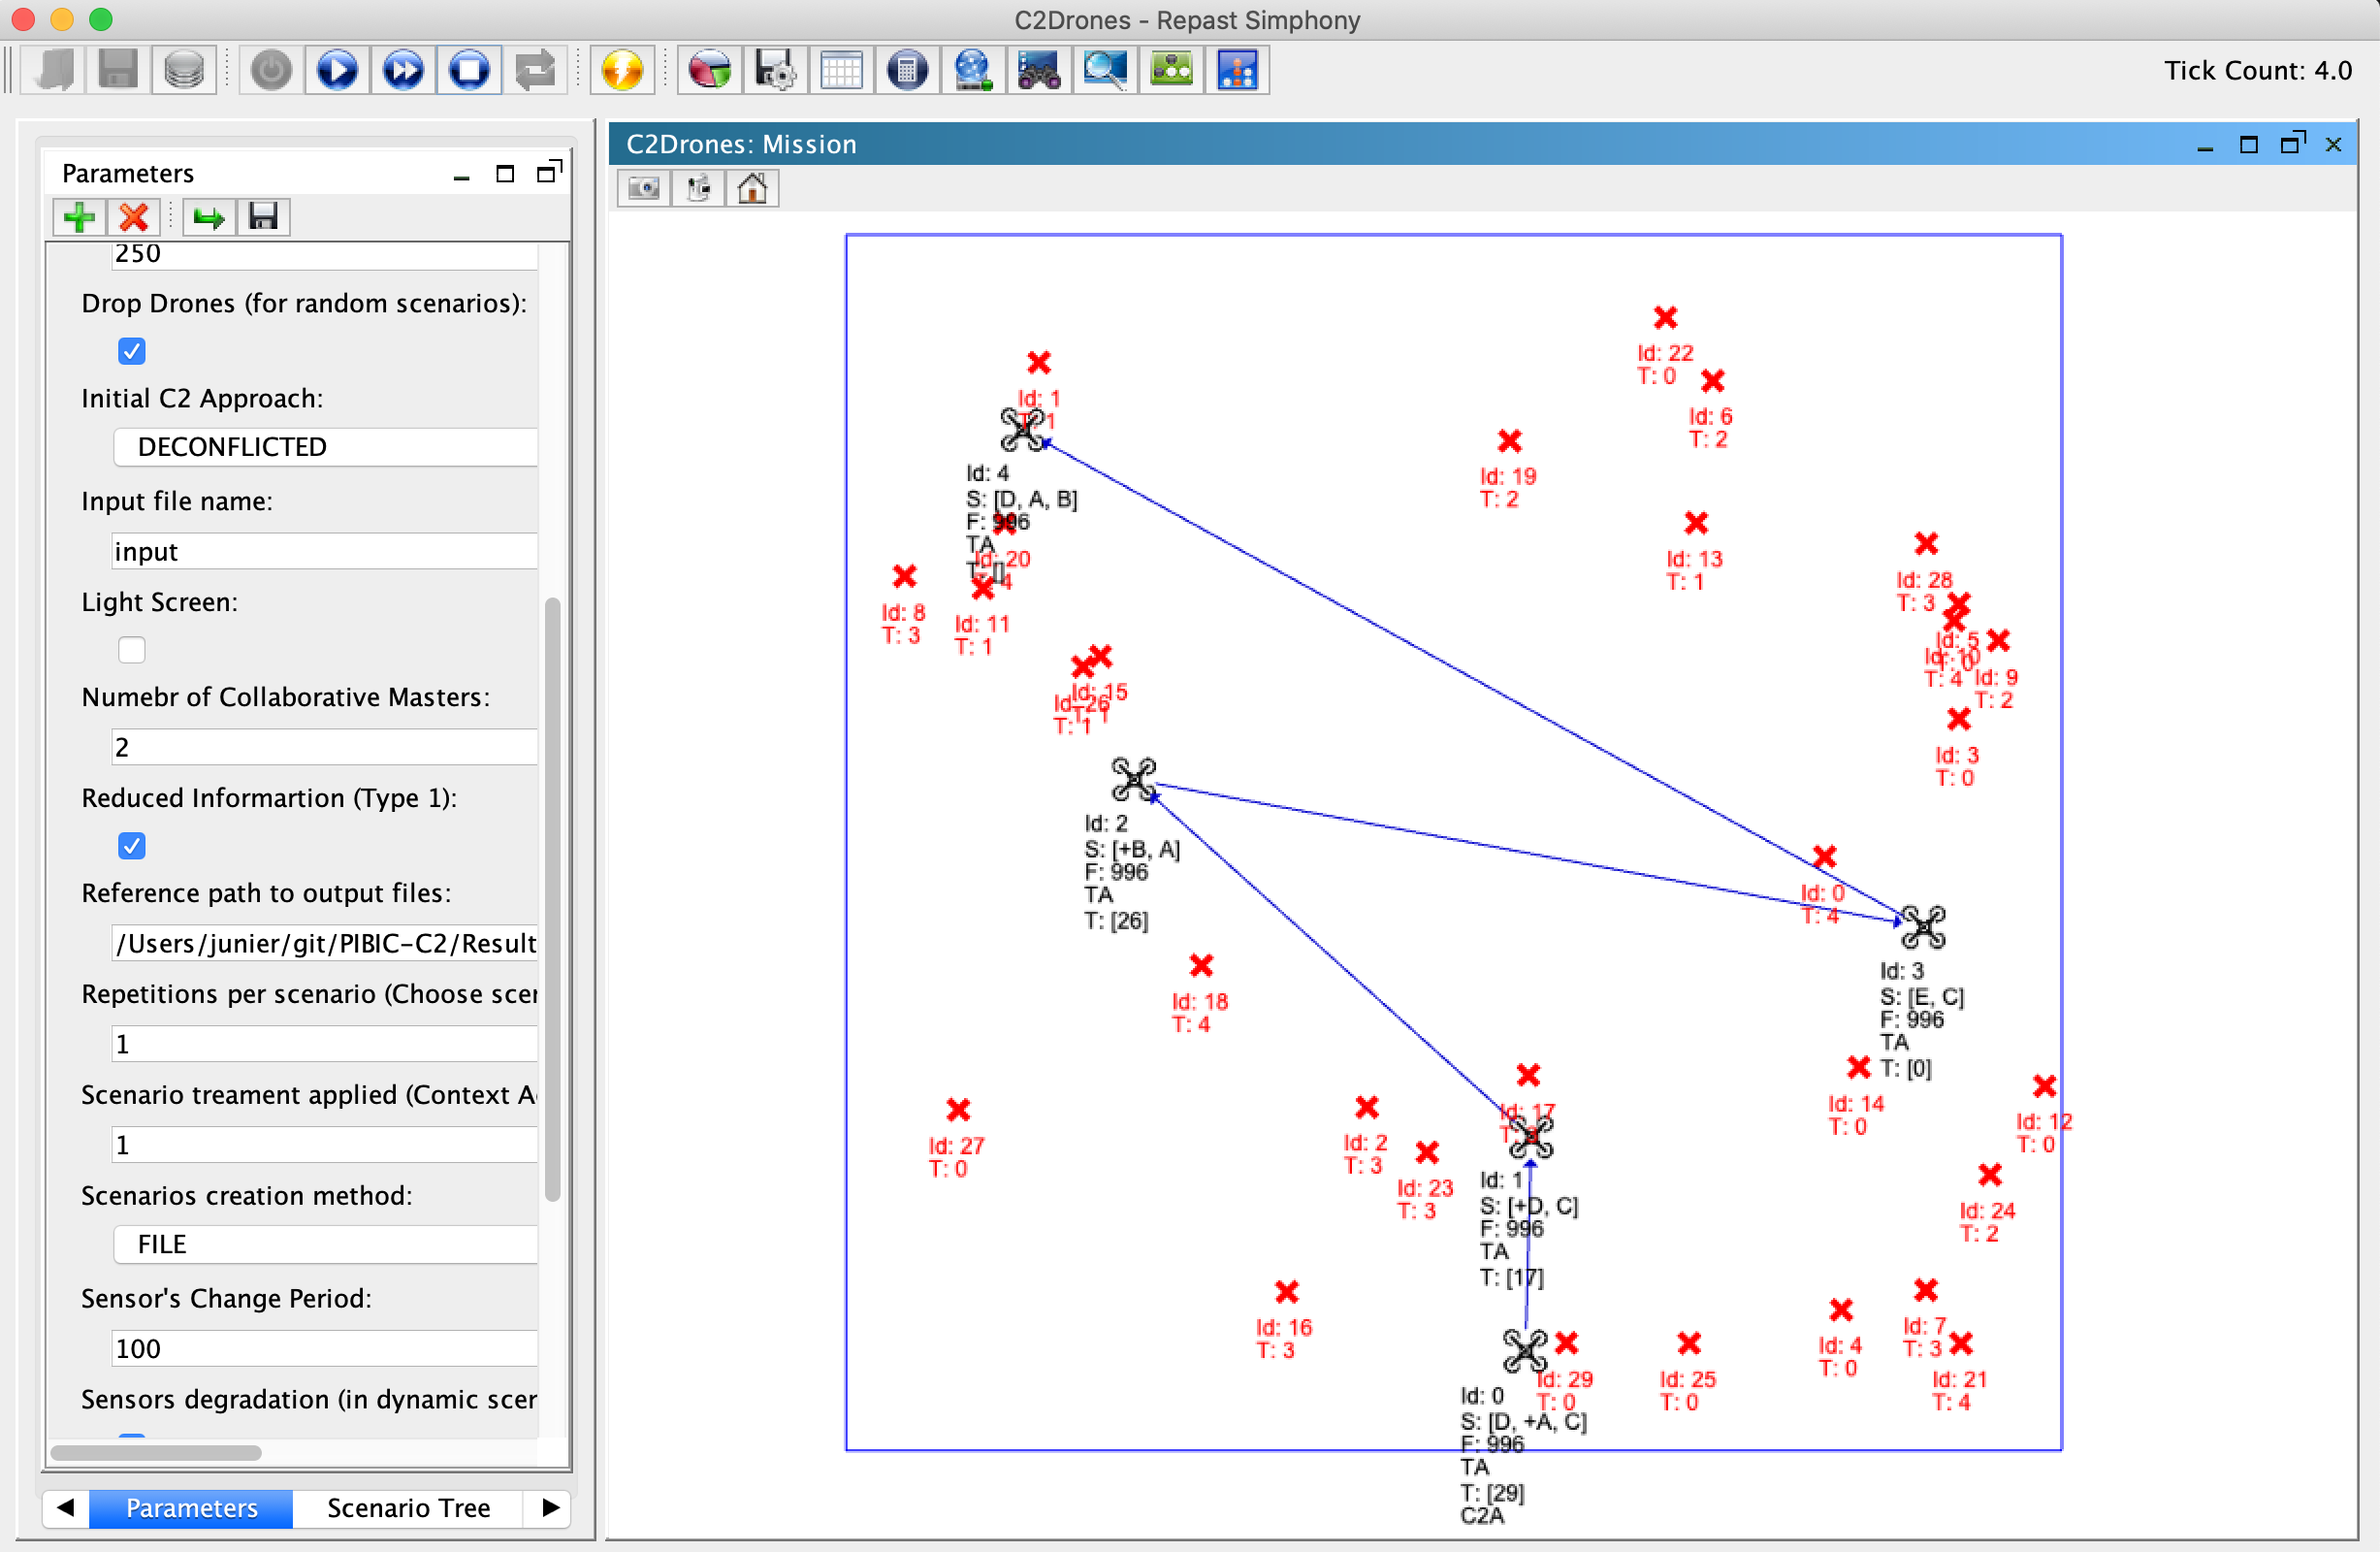
\includegraphics[width=0.7\linewidth]{img/repast01.png}
  \captionof{figure}{Simulator implementation  with Repast Simphony~\citep{SIMUL01}}
  \label{fig:repast01}
\end{figure}


The trials are performed feeding the simulator with the scenario data (cf. Section~\ref{sssec:scenarios}) combined with the two action methods shown in Figure~\ref{fig:exp_design}. Such scenarios are loaded through an input text file (CSV pattern). With all these data, the simulator runs each scenario with each action method, according to the experimental design (cf. Section~\ref{sssec:design}). The results are exported as text files and processed with \X{the R tool}~\citep{stat002,R_G} to calculate the mean and the standard deviation, draw graphs, and perform the statistical tests and validation.


%%%%%%%%%%%%%%%%%%%%%%%%%%%%%%%%%%
% SUBSECTION 
%%%%%%%%%%%%%%%%%%%%%%%%%%%%%%%%%%
\subsection{Executions}
\label{subsec:operations}

The experiment performs a significant set of executions in a batch way to reduce the effect of system startup on the standard deviation. An initial number of runs ($n_i=50$) was chosen to analyze the amount of dispersion in the results obtained by the experiments. Based on this, it was possible to observe the need to adjust the sample size to meet the acceptable confidence level (cf. Section~\ref{sssec:design}). According to \citet{CochranW.G.1983}, Equation~\ref{eq:stat} gives the sample size \emph{n} that satisfies a given confidence level, a population standard deviation $\sigma$, and the difference \emph{d} between the population mean ($\overline{X}$) and sample mean ($\mu$).

\begin{equation}
    \label{eq:stat}
    n=\left(\frac{Z_{\alpha/2} \cdot \sigma}{d}\right)^2
\end{equation}

According to the analysis procedure (cf. Section ~\ref{sssec:design}), the Equation~\ref{eq:stat} is applied with $95\%$ confidence, i.e., a $Z_{\alpha/2} = 1.96$, and $d = |\overline{X} - \mu| \leq 0.1\mu_i$, where $\mu_i$ is the mean obtained with the initial set of runs $n_i$. This value of $d$ is less than 10\% of the mean result obtained by the initial sample. With such parameters, an average sample size of 500 was obtained. Based on this, the factorial experiment with scenario and action method factors (see Figure~\ref{fig:exp_design}) was executed 500 times for all combinations of treatments. Table~\ref{table:results01} shows the results obtained for the metrics listed in GQM (Figure~\ref{fig:gqm}) for each scenario, which was performed 500 times. 

\begin{table}[ht]
	\small
	\fontsize{6.5}{6.5}\selectfont
	\centering
	\caption{Metrics results (Reconfigurations-M1, Maneuvering-M2, Engagement Time-M3, Effectiveness-M4, Resilience-M5 and Reward-M6)  after 500 executions of each scenario listed in Table~\ref{tab:scenarios} with the initial context of 5 members, 30 tasks, De-Conflicted as initial C2 Approach and a deadline of \color{black}1000 time ticks.\color{black}}
	\label{table:results01}
	
	\begin{tabular}{rrrrrrrr} \hline 
	    & \bf{M1}
		& \bf{M2}
        & \bf{M3}
        & \bf{M4}
		& \bf{M5}
		& \bf{M6} \\  \hline 
		
		& Mean(St.Dev.)  & Mean(St.Dev.) & Mean(St.Dev.)  & Mean(St.Dev.) & Mean(St.Dev.) & Mean(St.Dev.)  \\ [1ex]
		
		\multicolumn{7}{l}{\textbf{$\longrightarrow$ Scenario 1 }} \\
	% Scenario  1 
\bf{A1}  & 0.0 ($\pm$0.0)  & 0.0 ($\pm$0.0)  & 890.0 ($\pm$66.8)  & 82.0 ($\pm$5.9) & 97.5 ($\pm$1.0) & 20.7 ($\pm$1.7)  \\
\bf{A2}  & 17.5 ($\pm$1.7)  & 1.7 ($\pm$0.3)  & 945.5 ($\pm$33.1)  & 97.7 ($\pm$2.9)  & 99.9 ($\pm$0.1)  & 26.5 ($\pm$1.2)  \\ [1ex]
	
	\multicolumn{6}{l}{\textbf{$\longrightarrow$ Scenario 2 }} \\
% Scenario  2 
\bf{A1}  & 0.0 ($\pm$0.0)  & 0.0 ($\pm$0.0)  & 866.5 ($\pm$72.3)  & 77.5 ($\pm$6.3)  & 92.2 ($\pm$1.7)  & 20.0 ($\pm$1.7)  \\
\bf{A2}  & 18.1 ($\pm$2.1)  & 2.6 ($\pm$0.6)  & 934.0 ($\pm$33.0)  & 95.2 ($\pm$4.2)  & 97.3 ($\pm$1.3)  & 25.1 ($\pm$1.2)  \\ [1ex]
	
	\multicolumn{6}{l}{\textbf{$\longrightarrow$ Scenario 3 }} \\
% Scenario  3 
\bf{A1}  & 0.0 ($\pm$0.0)  & 0.0 ($\pm$0.0)  & 782.1 ($\pm$78.3)  & 63.7 ($\pm$5.5)  & 75.7 ($\pm$1.9)  & 16.1 ($\pm$1.3)  \\
\bf{A2}  & 15.4 ($\pm$1.7)  & 2.8 ($\pm$0.3)  & 883.0 ($\pm$49.2)  & 69.1 ($\pm$4.5)  & 70.7 ($\pm$2.3)  & 17.2 ($\pm$1.5)  \\ [1ex]
	
	\multicolumn{6}{l}{\textbf{$\longrightarrow$ Scenario 4 }} \\
% Scenario  4 
\bf{A1}  & 0.0 ($\pm$0.0)  & 0.0 ($\pm$0.0)  & 799.1 ($\pm$77.0)  & 63.6 ($\pm$5.3)  & 75.6 ($\pm$1.6)  & 16.4 ($\pm$1.3)  \\
\bf{A2}  & 18.2 ($\pm$2.3)  & 3.0 ($\pm$0.1)  & 913.4 ($\pm$35.9)  & 84.5 ($\pm$5.1)  & 86.4 ($\pm$2.4)  & 21.9 ($\pm$1.4)  \\ [1ex]
	
	\multicolumn{6}{l}{\textbf{$\longrightarrow$ Scenario 5 }} \\
% Scenario  5 
\bf{A1}  & 0.0 ($\pm$0.0)  & 0.0 ($\pm$0.0)  & 733.7 ($\pm$75.5)  & 54.6 ($\pm$4.6)  & 64.9 ($\pm$1.4)  & 13.9 ($\pm$1.2)  \\
\bf{A2}  & 16.1 ($\pm$2.0)  & 2.9 ($\pm$0.2)  & 887.7 ($\pm$48.4)  & 70.7 ($\pm$5.1)  & 72.3 ($\pm$2.9)  & 17.9 ($\pm$1.5)  \\ [1ex]
	
	\multicolumn{6}{l}{\textbf{$\longrightarrow$ Scenario 6 }} \\
% Scenario  6 
\bf{A1}  & 0.0 ($\pm$0.0)  & 0.0 ($\pm$0.0)  & 700.6 ($\pm$79.4)  & 42.0 ($\pm$4.5)  & 49.9 ($\pm$2.2)  & 10.7 ($\pm$1.1)  \\
\bf{A2}  & 15.0 ($\pm$2.0)  & 2.9 ($\pm$0.2)  & 910.5 ($\pm$59.3)  & 65.7 ($\pm$5.9)  & 67.2 ($\pm$3.9)  & 16.6 ($\pm$1.9)  \\ [1ex]
	
	\multicolumn{6}{l}{\textbf{$\longrightarrow$ Scenario 7 }} \\
% Scenario  7 
\bf{A1}  & 0.0 ($\pm$0.0)  & 0.0 ($\pm$0.0)  & 686.2 ($\pm$58.4)  & 41.1 ($\pm$3.5)  & 48.9 ($\pm$1.1)  & 10.9 ($\pm$1.0)  \\
\bf{A2}  & 15.0 ($\pm$2.0)  & 2.8 ($\pm$0.3)  & 820.5 ($\pm$61.4)  & 60.1 ($\pm$5.6)  & 61.5 ($\pm$3.7)  & 16.2 ($\pm$1.6)  \\ [1ex]
	
	\multicolumn{6}{l}{\textbf{$\longrightarrow$ Scenario 8 }} \\
% Scenario  8 
\bf{A1}  & 0.0 ($\pm$0.0)  & 0.0 ($\pm$0.0)  & 629.7 ($\pm$68.6)  & 36.3 ($\pm$3.8)  & 43.2 ($\pm$1.7)  & 9.1 ($\pm$0.9)  \\
\bf{A2}  & 13.0 ($\pm$1.5)  & 2.8 ($\pm$0.3)  & 785.1 ($\pm$58.3)  & 52.1 ($\pm$4.7)  & 53.3 ($\pm$3.1)  & 13.6 ($\pm$1.7)  \\ [1ex]
	
	\multicolumn{6}{l}{\textbf{$\longrightarrow$ Scenario 9 }} \\
% Scenario  9 
\bf{A1}  & 0.0 ($\pm$0.0)  & 0.0 ($\pm$0.0)  & 491.0 ($\pm$74.2)  & 26.4 ($\pm$3.7)  & 31.4 ($\pm$2.4)  & 7.0 ($\pm$1.0)  \\
\bf{A2}  & 15.5 ($\pm$1.6)  & 3.0 ($\pm$0.1)  & 743.2 ($\pm$66.1)  & 53.2 ($\pm$5.1)  & 54.4 ($\pm$3.4)  & 14.2 ($\pm$1.5)  \\ [1ex]
	
	\multicolumn{6}{l}{\textbf{$\longrightarrow$ Scenario 10 }} \\
		
% Scenario  10 
\bf{A1}  & 0.0 ($\pm$0.0)  & 0.0 ($\pm$0.0)  & 393.4 ($\pm$81.2)  & 24.3 ($\pm$2.6)  & 28.9 ($\pm$1.3)  & 6.2 ($\pm$0.9)  \\
\bf{A2}  & 11.4 ($\pm$1.4)  & 2.9 ($\pm$0.2)  & 650.7 ($\pm$114.8)  & 38.8 ($\pm$4.7)  & 39.7 ($\pm$3.4)  & 9.9 ($\pm$1.5)  \\ [1ex]
		\hline
	\end{tabular}
\end{table} 


%The simulation is not applying $addTask$ action due to the allocation task strategy adopted by the system, i.e., based on swarm algorithm, that puts the new task in the end of the available tasks list. Such position causes low impact in the system because the task will be allocated only if there is resources available after all previous allocation.


%%%%%%%%%%%%%%%%%%%%%%%%%%%%%%%%%%
% SUBSECTION 
%%%%%%%%%%%%%%%%%%%%%%%%%%%%%%%%%%
\subsection{Analysis and Discussion}
\label{subsec:analysis_discussion}


Table~\ref{table:results01} and Figures~\ref{fig:m1},~\ref{fig:m2},~\ref{fig:m3},~\ref{fig:m4},~\ref{fig:m5} and~\ref{fig:m6} show the results obtained by the simulation. Positive values for Reconfigurations (M1) (cf. Figure~\ref{fig:m1}) occur only in proposed method (A2) and indicates team's adaptation to deal with context changes in \color{black}all simulated scenarios\color{black}. By tracing into the source code of the simulation, we observed that such adaptations are followed by the tasks' reallocation activity in case the reconfiguration is not sufficient to make the member compatible with the task. A similar analysis can be applied to Maneuvering (M2) shown in Figure~\ref{fig:m2}. Positive values are obtained  only in the A2 method, which can perform a C2 Approach change to try a new awareness level. The values obtained show an upper bound due to the sequence of C2 Approach adopted starting from De-Conflicted up to Edge and finishing on the Conflicted one (cf. Section~\ref{ssec:background_c2}). 
%The values obtained show an upper bound due to the resource limitation to perform the mission, such as  members' fuel and time, which are spent during the C2 Approach change.

\begin{figure}
\centering
\begin{minipage}{.5\textwidth}
  \centering
  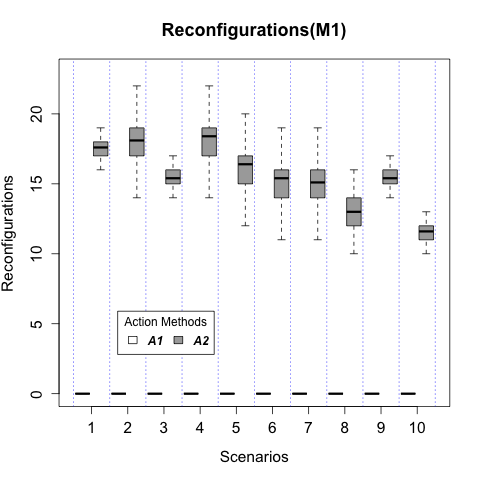
\includegraphics[width=0.95\linewidth]{img/graphs/Boxplot_M1.png}
  \captionof{figure}{Reconfigurations (M1)}
  \label{fig:m1}
\end{minipage}%
\begin{minipage}{.5\textwidth}
  \centering
  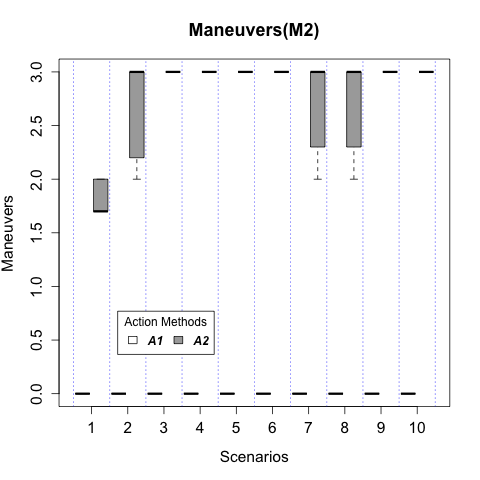
\includegraphics[width=0.95\linewidth]{img/graphs/Boxplot_M2.png}
  \captionof{figure}{Maneuvering (M2)}
  \label{fig:m2}
\end{minipage}
\end{figure}


Figure~\ref{fig:m3} shows results of Engagement Time (M3) for each scenario. In this case, the A2 method allows the system to keep running longer than A1, even in scenarios with more context changes. This suggests A2 provides more system availability due to its enhanced adaptation capability, as indicated by results for M1 and M2. 

 Regarding Effectiveness (M4), Figure~\ref{fig:m4} shows higher  capacity of the C2 system to solve tasks by the A2 method compared to A1, suggesting the higher availability obtained for M3 is well-employed in dealing with the mission in A2, increasing the system capacity to deal with context changes and to perform the tasks.


\begin{figure}
\centering
\begin{minipage}{.5\textwidth}
  \centering
  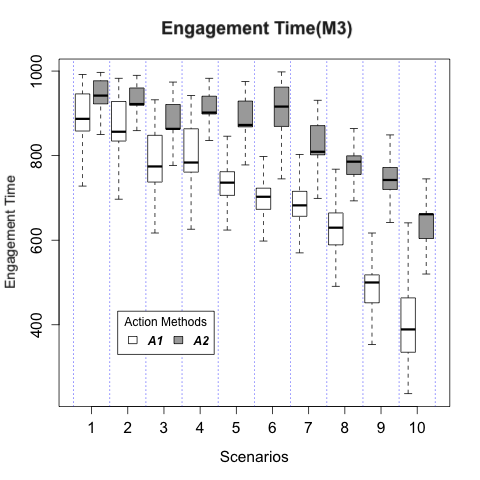
\includegraphics[width=0.95\linewidth]{img/graphs/Boxplot_M3.png}
  \captionof{figure}{Engagement time (M3)}
  \label{fig:m3}
\end{minipage}%
\begin{minipage}{.5\textwidth}
  \centering
  %  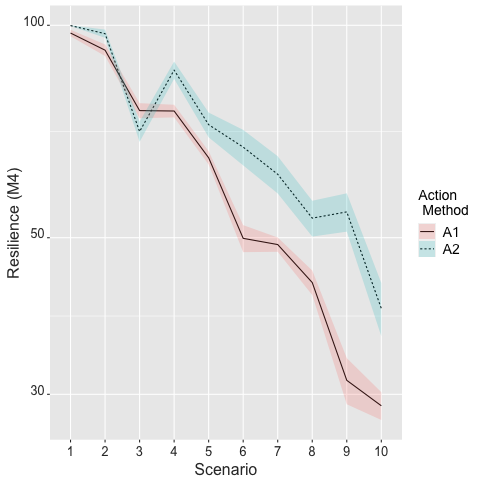
\includegraphics[width=0.95\linewidth]{img/graphs/Result_M4.png}
  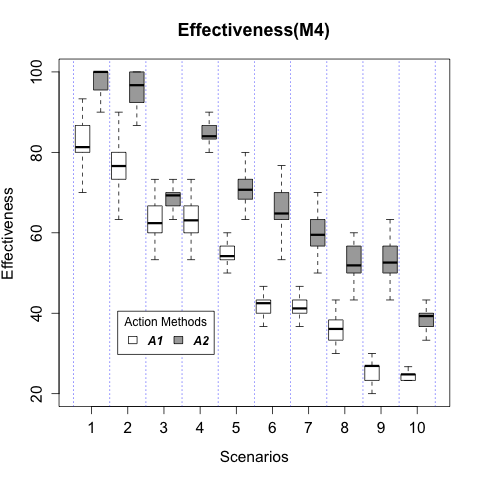
\includegraphics[width=0.95\linewidth]{img/graphs/Boxplot_M4.png}
  \captionof{figure}{Effectiveness (M4)}
  \label{fig:m4}
\end{minipage}
\end{figure}


Regarding the Resilience (M5) metric, Figure~\ref{fig:m5} shows that, in general, action method A2 is more capable of presenting a percentage of completed tasks closer to what would be obtained if the context remained unchanged. The only exception is for Scenario 3, since, upon exploration of simulation execution steps, the \emph{memberFailure} events in this scenario prompt task reallocation that cannot be better than the initial one made with the complete set of members. Besides, the time spent on members’ reconfiguration and tasks’ reallocation leads to a slightly lower result than that obtained by the A1 method, which only continues the execution.  

In terms of Reward (M6), Figure~\ref{fig:m6} shows better results for A2 indicating that the system adaptation provides more compatible configurations for performing tasks. Indeed, tracing into the simulation execution of method A2 reveals that all reconfiguration and C2 Approach change performed may lead to task reallocation. Such behavior always looks for the best member and sensor to perform the task to be allocated, reflecting the results presented in Figure~\ref{fig:m6}. In contrast, A1 performs only one allocation at mission startup. This way, when context change events occur, tasks are not \color{black}reallocated even when employed \color{black}sensors are damaged. Besides, if all 30 tasks in the mission are performed by the most compatible sensor for each one, i.e., with quality 1, we obtain the maximum result of 30 for reward (M6) metric. 
%Furthermore, as each sensor has a quality between 0 and 1 for each type of task, the maximum Reward metric (M6) that can be obtained is the sum of sensors' quality used, e.g., a total reward of 30 in a mission with 30 tasks using sensors with maximum quality level.



\begin{figure}
\centering
\begin{minipage}{.5\textwidth}
  \centering
  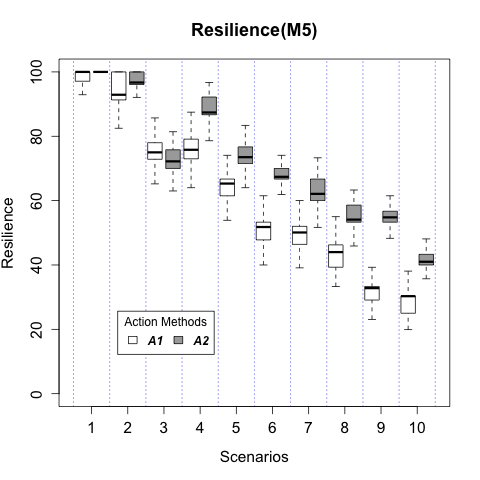
\includegraphics[width=0.95\linewidth]{img/graphs/Boxplot_M5.png}
  \captionof{figure}{Resilience (M5)}
  \label{fig:m5}
\end{minipage}%
\begin{minipage}{.5\textwidth}
  \centering
  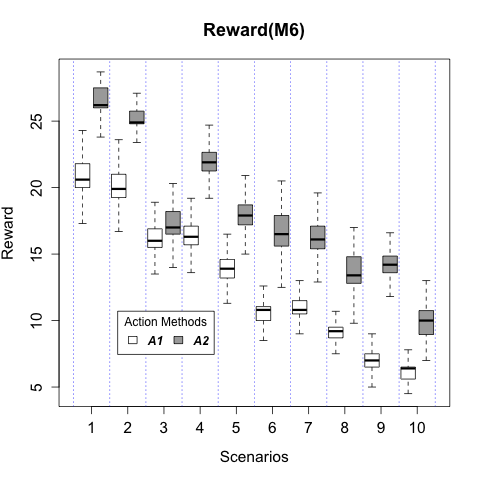
\includegraphics[width=0.95\linewidth]{img/graphs/Boxplot_M6.png}
  \captionof{figure}{Total reward (M6)}
  \label{fig:m6}
\end{minipage}
\end{figure}

Since removing members with the \emph{memberFailure} event does not allow members to reconfigure---prompting instead a task reallocation or even a C2 Approach change---it explains the decrease on M1, M4, M5, and M6 in Scenario 3 for method A2. \color{black}In contrast, \emph{sensorFailure} and \emph{envChange} enable member reconfiguration or change to the C2 Approach to search for an alternative allocation of pending tasks based on the algorithm used, i.e., swarm-gap based~\citep{MAS07, UAV01}, and the available context information. \color{black}It gives to A2 advantage in all other scenarios. Moreover, for methods A1 and A2, it is possible to observe a significant reduction in results for M3, M4, M5, and M6 due to the progressive loss of  system resources such as  members, sensors, and autonomy, as exercised by the scenarios. 

%Furthermore, the engagement time (M3) only suffered a significant decrease after a reduction in resources of more than 60\% identified from Scenario 6 onwards. 


%The \emph{null hypotheses $H_0$} in Table~\ref{table:hyp} can be refuted since the non-parametric statistical test demonstrated that the results of the metrics defined in GQM are different for the treatments applied to the action method. Even for Scenario 3, the \textit{p-value} for all metric were less than 0.05 and it indicates that the two samples compared, i.e., A1 and A2 results, are statistically different. Based on this, the alternative hypothesis is valid, confirming that the proposed method A2, able to perform internal reconfigurations and C2 Approach changes, presented a significant result in face of context changes simulated. We identify only Resilience (M5) metric in Scenario 3 with A1 results greater than A2 ones (cf. Figure~\ref{fig:m5}). These results evidence that the model proposed handles C2 Approach Agility (\emph{RQ1}) and C2 Maneuver Agility (\emph{RQ2}).

% Vander: after thinking about this the whole day, I fail to draw in my head any new info from comparing M3
% and M4. I suggest either simplifying a lot the following 3 paragraphs into a single one or
% removing the discussion. Operationally, I suggest: 1) consensus discussion; 2) Thiago writes the paragraph.
%
\color{black}
Nonetheless, even though both M3 and M4 decrease as scenarios become more complex, they do so at different rates.
Indeed, mean engagement time decreases less than 20\% before scenario 8, whereas mean effectiveness decreases about 46\% for the same scenarios (cf. Table~\ref{table:results01}).
This trend suggests that engagement time is not necessarily an indicator of effectiveness, strengthening the claim made by~\citet{Alberts2006} that ``the quality of C2 should not be deduced solely from mission outcomes''.
\color{black}


%The engagement time (M3) and the effectiveness (M4) metrics are complementary and highlights that the mission engaged does not show a direct ratio with its accomplishing. The main reason for this statement is the time spent by the entities to deal with context change, e.g., to find an appropriate allocation of remaining tasks. With the complexity of the events sequence that characterizes the context changes, it is possible to notice a significant reduction of M3, starting from scenario 7 as shown in Figure~\ref{fig:m3}, of about 40\% in the total time in ticks with our proposed model. Such decreasing is even bigger with no adaptation and coordination, i.e., with the action method A1. The context dynamism affects the M4 earlier, with a significant decreasing starting from scenario 3 (cf. Figure~\ref{fig:m4}) and getting up to 60\% of reduction in the percentage of completed tasks, in scenario 10.

%Even keeping long engagement in the mission, with negative impact only in complex scenarios with more change events, the overhead incurred by structure reorganization reduces the time for performing tasks. The number of C2 Approach changes (cf. Figure~\ref{fig:m2}), guided by the amount of context change events, causes reorganization of the members’ communication structure to continue executing the unfinished tasks and, because of this, causing a time-consuming. Based on this, comparing Figures~\ref{fig:m3} and~\ref{fig:m4}, we should have, conceptually, the engagement time in order to keep the effectiveness. However, we notice a time-consuming that reduces the number of complete tasks. In summary, the proposed modeling provided a higher percentage of mission completion (cf. Figure~\ref{fig:m4}), but there is a trade-off regarding the time taken to apply C2 agility.


%Even with a reduced decrease of less than 40\ when reaching the most complex scenario, i.e., the scenario 10, we faced a significant reduction of about 60\ in the effectiveness, i.e., the capacity of successfully executing tasks. In addition, comparing Figures~\ref{fig:m3} and~\ref{fig:m4}, we note a significant reduction of results in Scenarios 3 to 10 in the Engagement Time (M3) metric. These two scenarios present the maximum number of C2 Approach changes (cf. Figure~\ref{fig:m2}) because of the amount of context change events and the members’ need to reorganize the communication structure to continue executing the available tasks. Even keeping engaged in the mission, the overhead incurred by such reorganization reduces time for performing tasks. \color{black}

%Besides, as the members’ current task execution can be interrupted by a context change event, the effectiveness level (Figure~\ref{fig:m4}) drops faster than the engagement time (Figure~\ref{fig:m3}) since the total available execution time is limited by system’s resources and the mission execution deadline. Even with this decrease, it is possible to observe a considerable difference in these metrics’ values obtained with the system running the baseline action method A1 and the A2 proposed.
 


Although the difference between the results with action methods A1 and A2 for all scenarios and metrics is graphically observable, a statistical test was performed to confirm these differences. With a Shapiro-Wilk test~\citep{stat001}, a \textit{p-value} less than 0.05 was obtained, thus indicating a non-normal distribution. Accordingly, an Mann-Whitney U Test described in~\citet{stat002} was applied, i.e., Wilcoxon-test in R, to check differences among the samples of action methods A1 and A2 for all scenarios. According to the number and value of samples, the statistical analysis confirmed the difference between all results from A1 and A2 methods for all simulated scenarios. All  \emph{null hypotheses $H_0$} in Table~\ref{table:hyp} were then refuted in favor of the alternative hypotheses. A2 has statistically significant higher values for all metrics, except for Resilience (M5) in Scenario 3, in which case A1 has a 7\% higher value for the reasons discussed previously. Therefore, the simulation results provide evidence that the proposed model  provides C2 Approach Agility (\emph{RQ1}) and C2 Maneuver Agility (\emph{RQ2}).


\begin{center}
\fbox{\begin{minipage}{30em}
In summary, simulation results suggest that the proposed model exhibits C2 agility. Indeed, the system stays more time in action, completes more tasks and more compatible ones, resulting in higher resilience thereby better coping with context changes and perturbations in dynamic scenarios.

\end{minipage}}    
\end{center}



%%% REWRITING
%Despite the found evidence, this work presents some limitations that are related to the task allocation and the C2 Approach choice. The simulator performs a non-optimized task allocation and presents limited resilience in this process. Moreover, the selection of the C2 Approach occurs sequentially according to its communications structure. Such a choice does not take into account a previous analysis of the context. In this case, the several attempts of the C2 Approach have a cost in terms of operating time and onboard resources, impacting the obtained results.

%In addition, the C2 concepts are applied only in the computational environment, i.e., simulations. This application scenario may highlight restrictions to the extension of the proposed model to other domains and scenarios. Besides, the events that provide dynamism to the context considered in this work are suitable for UAV's operation scenarios. To extend the proposed model to other areas, making it more compatible with real scenarios, it is necessary to include new events that may impact the model's behavior and may require significant adjustments.








\section{Threats to Validity}
\label{sec:threats}
%Threats to validity

Since the simulation presented in Section~\ref{sec:evaluation} was performed to assess the proposed model in Section~\ref{sec:proposal}, the following mitigation strategies were adopted to address the corresponding threats to validity: 

\begin{itemize}
   \item \textbf{Conclusion validity}: The execution scenarios involve random variables that provide different results with significant dispersion. To account for variance in the experiment environment, each factorial experiment combining scenarios and action methods was executed 500 times to reduce the standard deviation. Besides, in cases where the metrics for different action methods (A1 and A2) were equal to each other, a non-parametric test was applied to identify these minor differences among the results obtained to assess the system embedded agility. Such a test was chosen due to the non-normal distribution of the samples obtained from the experiments.
   
   
   \item \textbf{Internal validity}: The CS implementation performed by this work can obtain different results according to the allocation algorithm used and the strategy of C2 approach selection. To mitigate this threat, some well-known strategies were followed to allocate tasks inspired in swarm intelligence~\citep{MAS07, UAV01}. To perform the C2 Approach change, we followed the maturity scale proposed by~\citet{nato01}. This strategy is well known and recognized by the military domain in many real and simulated scenarios~\citep{FRANCE2014}. Furthermore, a simple implementation was performed to avoid technology dependence in results.
   
   
   \item \textbf{Construct validity}: To assure that the metrics chosen for the evaluation are suitable measures of the issue under investigation, they were derived from the C2 Agility attributes presented by~\citet{Alberts2006} and~\citet{nato01}. Additionally, the event changes that characterize a dynamic scenario are grounded on real military scenarios~\citep{UAV_Aplication, Power01}, and confirmed with domain experts.
   
  % Reviewer 2: Seems like another approach would be to come up with distributions of different kinds of events (perhaps provided by domain experts when actual data from real-world operations are not available) and randomly select the sequence based on those distributions. One wonders how such an approach would effect the results, or even how sensitive the results might be to the distributions. Maybe add some discussion of this if you think it would provide additional weight to these validity arguments.
  % The events’ order or even their kinds could affect the system’s response and it might become the analysis harder, generating outliers or not normalized results. To provide better conditions for analyzing the system response, we order the events under rules defined by domain experts to simulate a complexity increasing scenario.
  % To provide better conditions for analyzing the system response, we order the events under rules defined by domain experts to simulate a complexity increasing scenario.
   
   \item \textbf{External validity}: The events shown in Table~\ref{table:context_changes} are a small set of possible changes and perturbations under which a real system can be placed. Additionally, the sequence of changes used to create the scenarios and described in Table~\ref{tab:scenarios} can have a countless number of possibilities. To mitigate such a threat, this work considers events and increasingly complex scenarios that are well known in the military domain. \X{Based on this, the events’ order or even their kinds could affect the system’s response and it might become the analysis harder, generating outliers or not normalized results. A previous experiment with this set of events randomly chosen showed random results distribution and was difficult to analyze.} Besides, the role-based modeling used by this work explores the organization of responsibilities among entities and such strategy is applied by other domains cited in Section~\ref{sec:example}. Moreover, due to the fact that it involves elements related to human behavior, such as leadership~\citep{Alberts2006}, normally the strategies adopted to deal with this dynamism focus on historical data or hit-and-miss based on the context information available in order to provide a timely response. In general, it is possible to observe low maturity regarding to C2, given its complexity and multi-disciplinarity. In interviews and by collecting information from experts in the military domain (Brazilian Army), they confirmed the compatibility of the adopted treatments, i.e. A1 and A2, and realistic scenarios. Additionally, the results in ~\citet{UAV01} confirms the effects of dynamism using simulations and it uses a procedure similar to the A1 strategy. 
   % RELACIONADO À EXTRAPOLAÇÃO (APLICAÇÃO EM OUTROS CENÁRIOS)
   % FAZER O PARALELO DO DOMÍNIO MILITAR E A APLICAÇÃO EM OUTROS DOMINIOS CITADOS NA MOTIVAÇÃO DO TRABALHO.
   
\end{itemize}





\section{Related Work}
\label{sec:relatedWork}
\citet{FRANCE2014}, in the North Atlantic Treaty Organization (NATO) context, performed research to improve C2 agility in military operations. To collect evidence to support some identified hypotheses, they leveraged simulation-based experiments and retrospective case studies of real operations. Similar to our study, the simulations created a dynamic context to assess the entities' response. Differently, they did not address any cost notion in the simulated environment. Considering  time, entities' fuel, or other resources is essential because they influence the  obtained results in the mission accomplishment, in the worst case  making it unfeasible. Such analysis was left as an opportunity for future work and this is the focus of our study.

\citet{Swart2012} shows C2 as a set of processes that manipulates information and data through a network structure and does not describe the entities themselves involved with such processes. \X{Such a modeling does not provide a strategy to represent the entities' behavior.} Our study seeks to fill this gap.~\citet{Mason2001} proposed a software architecture that can model a headquarters applying C2 processes in a military operation. Those studies, however, did not address the system response level in a dynamic context, which is addressed in our work.

\citet{Stanton2007} presented Process Model as a structure that summarizes the monitoring, decision making,  adaptation, and action executed by the C2 process to deal with context changes. Nonetheless, such a model does not show entities' behavior and relation during the mission under context change effects. Based on this and the concept of C2 Agility presented by~\citet{Alberts10}, our study proposes a model applied to the C2 process to deal with new constraints and conditions caused by dynamic contexts. 

\citet{c2-02} provided simulation-based evidence that adaptive networks can provide C2 Agility. 
Such work addresses only the network structure, not exploring the members' adaptation, i.e., network elements, in case of circumstance changes. In contrast, our work proposes a model that addresses C2 Agility in two levels, one in terms of network structure and the second where there is an adaptation by \color{black}member reconfiguration \color{black}or task reallocation.\color{black}~\cite{UAV01} demonstrates dynamism relevance with simulations, submitting different scenarios to C2 Agility treatment and collecting metrics. We leverage such dynamic scenarios with comparison treatments to evaluate C2 Agility results.\color{black}

\citet{SAS04} shows that Self-Adaptive Systems (SAS) can adapt themselves to satisfy new requirements from the environment or the user. This characteristic has \color{black}similar principles to C2 Agility \color{black}where adaptation is a requirement to deal with context changes. However, this adaptation is only related to the systems' configuration. There is no coordination aspect involved, which would be related to C2 Maneuver Agility.

\citet{Rosenmuller2011} describe a Dynamic Software Product Line (DSPL) as an approach to model a SAS.
Moreover, \citet{BSN-DSPL} present techniques to ensure the reliability of such DSPL, which is a relevant quality aspect in critical domains.
These product-line design and verification methods can be leveraged to systematically handle the reconfiguration of team members in our setting.
However, we consider that the specifics of such techniques are implementation details, which are abstracted by functions \texttt{reconfig} and \texttt{find\_configuration} in the program graph for the TP role (Figure \ref{fig:ex_pg}).


According to~\citet{Rutten2017}, an automaton can be used to model SAS behavior. Besides, multiple automata can be connected forming a network and representing a set of components. \citet{MC01} show that such automata can be written as a Transition System (TS) with a finite number of states represented by Labeled Kripke Structures. As \citet{ltl02} use TS to model DSPLs, we may apply such structure to model C2 entities. However, modeling directly in this structure can become unfeasible due to a \color{black}prohibitive number \color{black}of states. To address this limitation, \citet{MC01} present the program graph abstraction.   \color{black}We leverage this \color{black}to model the behavior of entities that are part of a C2 System. We further leverage the parallel composition --channel system-- of these program graphs with a type-parameterized extension to achieve C2 Agility. 

%these program graphs are used to model roles, i.e., an abstraction of the entities' behavior that is part of a C2 structure. An agent can play one or more instances of a role. Based o this, \citet{agent0010} shows the use of roles as components of agents' implementation for modeling communication and coordination of an agent-based system~\citep{agent1}. These agents can accumulate different types of roles and responsibilities and execute them according to the circumstance~\citep{weyns2019activforms}.


Empirical studies with the use of simulation are widely explored and they are relevant to many different domains, e.g., \color{black}military~\citep{CC03} and \color{black}environmental monitoring~\citep{simulation001}. The simulation can create several circumstances to evaluate a solution or product, or to train professionals, reducing the need for resources to create real circumstances. In line with this philosophy and based on the comparison presented by~\citet{SIMUL01}, we have chosen Repast Simphony as the simulation environment and tool to perform tests and collect evidence related to our theory due to the technology usability and previous experience with the underlying Java technology. In general, the implementation of this work was based on strategies presented by~\citet{MAS07} and \citet{UAV01} where UAVs perform a reconnaissance mission. However, we extended the agent-based simulation to include the Maneuver Agility concept combined with team members' reconfiguration.




\section{Conclusion} 
\label{sec:conclusion}
C2 refers to mobilizing entities' efforts to the achievement of a goal and has been applied in a myriad of domains, across which dynamism abounds. A key requirement in these applications is C2 agility, which is the capability of the entities to deal with dynamic situations,  managing resources to achieve a timely and suitable C2 system response. Nevertheless, there is a lack of solutions on how to provide C2 agility to deal with dynamic contexts.

To demonstrate how C2 agility may be handled, we propose a computational model of a C2 System composed of entities collaborating towards completing a mission. The model defines how entities' reconfiguration and coordination may help handle context changes occurring in the mission, in the environment, or in the entities themselves. The C2 System model is formalized as a typed-parameterized extension of a channel system, which defines the roles and responsibilities handled by the entities constituting a C2 System, where each entity is modeled as a dynamic software product line. 


%This work extends the Channel System concept to propose a C2 Agility model based on behavior representation using Program Graphs. The entities have one or more different overlapping roles, and they can exchange information among them. This typed-parameterized model combines the reconfiguration and the coordination capabilities of the entities that play different roles, which are represented as program graphs. Besides, all artifacts related to our study are publicity available~\footnote{\gitRepository}.

%This typed-parameterized model uses channels to provide the necessary data and message exchange between roles. Such communication is essential to provide the coordination defined as a C2 principle. Furthermore, the Software Product Line (SPL) approach applied to model the members, implementing them as DSPL, guaranteed a self-configuration to optimize resources application to deal with context changes and to keep performing the mission. As SPL, the entities' onboard software is generated from features activated or not, reusing quality and previous structure. 


Simulation results suggest that the proposed model exhibits C2 agility. Indeed, the system spends more time in action, completes more tasks and more compatible ones, resulting in higher resilience thereby better coping with context changes and perturbations in dynamic scenarios.

Despite the shown evidence, this work presents some limitations that are related to the task allocation and the C2 Approach choice. The simulator uses a non-optimal algorithm based on swarm-gap strategy, with limited resilience, to perform a suitable allocation according to the context information available in the token. Moreover, the selection of the C2 Approach occurs sequentially according to its communications structure. Such a choice does not take into account a previous analysis of the context. In this case, the several attempts of the C2 Approach have a cost in terms of operating time and onboard resources, impacting the obtained results.

Furthermore, the C2 concepts are applied only in the computational environment, i.e., simulations. This application scenario may highlight restrictions to the extension of the proposed model to other domains and scenarios. Besides, the events that provide dynamism to the context considered in this work are suitable for UAV operation scenarios. To extend the proposed model to other areas, making it more compatible with real scenarios, it is necessary to include new events that may impact the model's behavior and may require significant adjustments.

Future work can explore the use of elaborated solutions applied to the function of maneuvering search and task allocation, \X{including the scenarios with restricted or compromised communications.} One possibility is the use of machine learning to process data collected from sensors in order to select the most suitable configuration and coordination structure. This Artificial Intelligence (AI) system can be improved with human activities controlling the start of any action, i.e., human-in-the-loop (HITL) strategy, or something more autonomous as human-on-the-loop~\citep{HITL01}. The proposed model can absorb any of these strategies to provide better results related to the mission execution in a dynamic context. Such a human collaboration is relevant because some C2 functions are related to behavior, e.g., leadership. In addition, other metrics, in particular those related to agility, e.g., robustness and innovation, can be inserted to make a deeper analysis regarding agility. \X{In addition, it is possible to perform a broader number of experiments with different scenarios, enlarging the domain scope with different number of entities, tasks, or changing events, in order to evaluate their effects and the system’s response to face a larger and more distinct number of context changes. Thus, we may insert new events into the CS through new actions that cause the expected effect on the system according to the context change that occurred.}

%Future work can explore the use of elaborated solutions applied to the function of maneuvering search and task allocation. One possibility is the use of machine learning to process data collected from sensors in order to select the most suitable configuration and coordination structure. This strategy can be plugged into the proposed model to provide better results related to the mission execution in a dynamic context. In addition, other metrics, in particular those related to agility, e.g., robustness and innovation, can be inserted to make a deeper agility analysis. 


% @TODO: remember to insert acknowledgments

%\section*{References} %it was removed because the bibliography tag (in elsarticle class) includes this label in the text.
%\bibliographystyle{elsarticle-num}
%\bibliographystyle{elsarticle-num-names}
%\clearpage
\bibliography{references}
\bibliographystyle{model5-names}
\biboptions{authoryear}
%\bibliographystyle{addons/model5-names}
%\biboptions{authoryear}
%\bibliographystyle{plainnat}
%\biboptions
\end{document}